%%%%%%%% ICML 2022 EXAMPLE LATEX SUBMISSION FILE %%%%%%%%%%%%%%%%%

\documentclass[12pt]{article}

% Recommended, but optional, packages for figures and better typesetting:
\usepackage{natbib}
\usepackage{microtype}
\usepackage{graphicx}
\usepackage{subfigure}
\usepackage{booktabs} % for professional tables
\usepackage{fullpage}
\renewcommand{\baselinestretch}{1.35}
% hyperref makes hyperlinks in the resulting PDF.
% If your build breaks (sometimes temporarily if a hyperlink spans a page)
% please comment out the following usepackage line and replace
% \usepackage{icml2022} with \usepackage[nohyperref]{icml2022} above.
%\usepackage{hyperref}

\usepackage[breaklinks,colorlinks,
            linkcolor=red,
            anchorcolor=blue,
            citecolor=blue
            ]{hyperref}
% Attempt to make hyperref and algorithmic work together better:
\newcommand{\theHalgorithm}{\arabic{algorithm}}

% Use the following line for the initial blind version submitted for review:
%\usepackage{icml2022}

% If accepted, instead use the following line for the camera-ready submission:
% \usepackage[accepted]{icml2022}

% For theorems and such
\usepackage{amsmath}
\usepackage{amssymb}
\usepackage{mathtools}
\usepackage{amsthm}
\usepackage{algorithm}
\usepackage{algorithmic}
\usepackage{enumitem}
% if you use cleveref..
\usepackage[capitalize,noabbrev]{cleveref}

%%%%%%%%%%%%%%%%%%%%%%%%%%%%%%%%
% THEOREMS
%%%%%%%%%%%%%%%%%%%%%%%%%%%%%%%%
\theoremstyle{plain}
\newtheorem{theorem}{Theorem}[section]
\newtheorem{proposition}[theorem]{Proposition}
\newtheorem{lemma}[theorem]{Lemma}
\newtheorem{corollary}[theorem]{Corollary}
\theoremstyle{definition}
\newtheorem{definition}[theorem]{Definition}
\newtheorem{assumption}[theorem]{Assumption}
\newtheorem{remark}[theorem]{Remark}

% Todonotes is useful during development; simply uncomment the next line
%    and comment out the line below the next line to turn off comments
%\usepackage[disable,textsize=tiny]{todonotes}
\usepackage[textsize=tiny]{todonotes}


\usepackage{relsize}
\usepackage[utf8]{inputenc} % allow utf-8 input
\usepackage[T1]{fontenc}    % use 8-bit T1 fonts
\usepackage{url}            % simple URL typesetting
\usepackage{booktabs}       % professional-quality tables
\usepackage{amsfonts}       % blackboard math symbols
\usepackage{nicefrac}       % compact symbols for 1/2, etc.
\usepackage{microtype}      % microtypography
\usepackage{smile}
\usepackage{bbm}
\usepackage{xcolor}
\usepackage{bbm}
\def \d {\text{d}}
\def \mcs{\mathcal{S}}
\def \mcm{\mathcal{M}}
\def \mbp{\mathbb{P}}
\def \mcd{\mathcal{D}}

\newcommand{\jiyuan}[1]{{\color{cyan} Jiyuan: #1}}
%%%%%%%%%% Start TeXmacs macros
\newcommand{\nobracket}{}
\newcommand{\tmcolor}[2]{{\color{#1}{#2}}}
\newcommand{\tmmathbf}[1]{\ensuremath{\boldsymbol{#1}}}
\newcommand{\tmop}[1]{\ensuremath{\operatorname{#1}}}
\newcommand{\tmrsub}[1]{\ensuremath{_{\textrm{#1}}}}
\newcommand{\tmtextit}[1]{\text{{\itshape{#1}}}}
\newcommand{\tmtextrm}[1]{\text{{\rmfamily{#1}}}}
\newcommand{\tmstrong}[1]{\textbf{#1}}
%%%%%%%%%% End TeXmacs macros


% The \icmltitle you define below is probably too long as a header.
% Therefore, a short form for the running title is supplied here:
%\icmltitlerunning{Pessimistic Minimax Value Iteration: Provably Efficient Equilibrium Learning from Offline Datasets}
\title{\LARGE Estimation of Treatment Effects in Extreme and Unobserved Data}
\author{Jiyuan Tan\thanks{Jiyuan Tan was partially supported by NSF Award IIS-2337916.} \quad 
  Jose Blanchet \quad 
  Vasilis Syrgkanis\thanks{Vasilis Syrgkanis was supported by NSF Award IIS-2337916.} 
  }
\date{}
\begin{document}
\maketitle
% This problem is encountered frequently in a wide range of areas, including policy evaluation, healthcare, education, and business decision-making. 

\begin{abstract}
Causal effect estimation seeks to determine the impact of an intervention from observational data. However, the existing causal inference literature primarily addresses treatment effects on frequently occurring events. But what if we are interested in estimating the effects of a policy intervention whose benefits, while potentially important, can only be observed and measured in rare yet impactful events, such as extreme climate events? The standard causal inference methodology is not designed for this type of inference since the events of interest may be scarce in the observed data and some degree of extrapolation is necessary. Extreme Value Theory (EVT) provides methodologies for analyzing statistical phenomena in such extreme regimes. We introduce a novel framework for assessing treatment effects in extreme data to capture the causal effect at the occurrence of rare events of interest. In particular, we employ the theory of multivariate regular variation to model extremities. We develop a consistent estimator for extreme treatment effects and present a rigorous non-asymptotic analysis of its performance. We illustrate the performance of our estimator using both synthetic and semi-synthetic data. 
\end{abstract}



\section{Introduction}
We are interested in studying the effect of treatment e.g., different policies and drugs, on rare yet impactful events such as large wildfires, hurricanes, tsunamis and climate change.  These kinds of events happen at an extremely low frequency, but they can cause considerable damage to properties and pose serious threats to people's lives. For instance, we may want to know the effect of more infrastructure investment or other kinds of precautions policies on earthquakes. In many applications – from financial risk to environmental policy – it isn’t enough to know how a treatment changes the average outcome; decision-makers care about whether it alters the extreme tail. More formally, we may want to estimate the effect of treatment $D$ on outcome $Y$ conditioning on some extreme events. Estimating this kind of effect can help policymakers evaluate the impact of a policy and choose the best policy to reduce economic loss and save more lives when disasters happen. 

\noindent\textit{Remark (notation).} $D\in\{0,1\}$ denotes the treatment indicator. In Lemma~\ref{lemma:mu_rate}: In the proof's expansions $f(t)=C\beta t^{-\beta-1}(1+D(1-1/\beta)t^{-1}+o(t^{-1}))$ and $\bar F(t)=Ct^{-\beta}(1+Dt^{-1}+o(t^{-1}))$, $D$ denotes a fixed expansion coefficient rather than the treatment indicator. $Y$ is the observed outcome satisfying consistency $Y=Y(D)$, where $Y(d)$ denotes the potential outcome when treatment is set to $d$.


Despite its clear importance, existing methods fall into two largely disconnected strands, each of which cannot fully address this question. One approach comes from the causal inference literature. Causal inference provide a comprehensive framework for counterfactual reasoning. Causal effect estimation is an important problem in this area, which finds wide applications in healthcare, education, business decision-making, and policy evaluation.  Classic causal inference literature mainly focuses on estimating the average effects among certain groups. Little attention is paid to the causal effect on rare events. The scarcity of extreme data makes inference more challenging than in classic settings. As a result, naively applying classic causal inference estimation methods will produce poor results with large statistical error.  For example, when making policies about earthquakes, we are usually unable to see a strong signal from historical data, as large earthquakes rarely occur and there are fewer samples in the dataset.

On the other hand, the Extreme Value Theory (EVT) studies the tail behaviors for statistical distributions, which provides the ideal tools for analyzing rare events. However, this approach does not take the data structure into consideration. In particular, it does not accommodate counterfactual treatments or adjust for covariates, so it cannot tell us what would happen under an intervention. 

To bridge these gaps, we combine causal inference theory with EVT to provide a novel framework for extreme effect measurement. Following researches in EVT \cite{coles2001introduction}, we use a multivariate regularly varying variable $U$ to model extremity. The rare event can be modeled by the event $\{\|U\| > t\}$ for large $t$. Our proposed estimand can be viewed as the Average Treatment Effect (ATE) conditioning on $\{\|U\| > t\}$ with rescaling as $t$ increases to infinity. Detailed definition and explanation can be found in Section 3. Estimation is challenging because the limiting tail distribution is unknown and must be inferred from finite samples. To improve data efficiency and inference accuracy, we combine tail observations with moderate‐frequency data in an extrapolation scheme, leveraging EVT insights alongside causal‐inference techniques to achieve efficient estimation.

\noindent\textit{Remark (notation).} $U$ denotes the extreme-noise vector in $\mathbb R_+^d$, with $\|U\|=\|U\|_1$ throughout the treatment-effect analysis. In Lemma~\ref{lemma:mu_rate}, Lemma~\ref{lemma:eta_rate}: Assumption~\ref{assump:mvary} specifies the noise law $\mathcal L(U)$, with $U=AZ$ and $m=d_z$ in the component density. In Theorem~\ref{thm:rate}, Lemma~\ref{lemma:eta_ipw}: Assumption~\ref{assump:mvary} specifies the noise law $\mathcal L(U)$, with $U=AZ$ and $m=d_z$ in the component density. $t>0$ is the level defining the strict exceedance event $\{\|U\|_1>t\}$, except when it is the argument of a scalar function in a tail calculation. In Proposition~\ref{prop:id}: $t$ is a deterministic limit parameter tending to infinity. In Theorem~\ref{thm:rate}, Lemma~\ref{lemma:eta_rate}, Lemma~\ref{lemma:eta_ipw}: The finite-threshold analysis uses a fixed deterministic $t$. In Corollary~\ref{cor:rate}, Corollary~\ref{cor:rate_ipw}: The selected threshold is $t=t_n$, with $c_-n^{\kappa(\hat\gamma_n)}\leq t_n\leq c_+n^{\kappa(\hat\gamma_n)}$, where $0<c_-\leq c_+<\infty$ are deterministic and independent of $n$ and the observed sample. Here $\kappa(v)=(1-2s)v$ when $s\in(0,1/(2+\max\{1,\beta\}))$, and $\kappa(v)=v/(1+2\min\{1,v\})$ when $s\in[1/(2+\max\{1,\beta\}),1/2)$. The threshold-indexed nuisance and conditional-moment conditions hold jointly for every deterministic $t\in I_n=[(c_-/2)n^{\kappa(\gamma)},2c_+n^{\kappa(\gamma)}]$. In Lemma~\ref{lemma:eta_rate}: The bound concerns sufficiently large $t\geq1$, subject to $n\pi_t\geq16\log(4/\delta)$, where $\pi_t=\mathbb P(\|U\|>t)$. In Lemma~\ref{lemma:eta_ipw}: The bound concerns sufficiently large $t\geq1$, subject to $n\pi_t\geq16\log(4/\delta)$, where $\pi_t=\mathbb P(\|U\|>t)$. In Theorem~\ref{thm:rate}: The main bounds concern deterministic $t\geq t_W$, subject to $n\pi_t\geq16\log(12/\delta)$, where $\pi_t=\mathbb P(\|U\|>t)$; the additional simplified bounds also require $t\geq\exp(1)$ and $a\log t\leq1$, where $a=R_\alpha(n,\delta/12)$.


To the best of our knowledge, we are not aware of any work in the literature that considers this problem. In this paper, we take the first step to measure the treatment effect on extreme events. To be more specific, our contributions can be summarized as follows. 

\begin{enumerate}
    \item We propose a measure for the treatment effect on rare events named Normalized Extreme Treatment Effect (NETE), which essentially measures the magnitude of treatment on tailed events.  
    \item We develop two consistent estimators for NETE—a doubly robust (DR) estimator and an inverse propensity weighting (IPW) estimator—by combining recent advances in multivariate tail–dependence estimation \cite{zhang2023wasserstein} with double machine learning methodology \cite{chernozhukov2018double}, and derive finite‐sample, non‐asymptotic error bounds.
    \item Synthetic and semi-synthetic experiments demonstrate a good practical performance of our proposed estimator as compared to baseline estimators adapted from standard causal inference literature. 
\end{enumerate}

\paragraph{\textbf{Related Work}} We briefly review some relevant literature in EVT and causal inference. \cite{coles2001introduction} provides a comprehensive introduction to EVT. A large amount of work focuses on the univariate setting \citet{davisonModelsExceedancesHigh1990,leadbetterBasisPeaksThreshold1991,pickandsiiiStatisticalInferenceUsing1975,smithExtremeValueAnalysis1989}. Recently, there have been many recent works on the multivariate generalization of these results \cite{avella2022kernel,zhang2023wasserstein}. Causal effect estimation is a classical problem in causal inference \citep{rubin1974estimating}.  
Common estimators include IPW \citep{rosenbaum1983central},  
DR methods \citep{bang2005doubly, kang2007demystifying,chernozhukov2016double,chernozhukov2017double,chernozhukov2018double},    
Targeted Maximum Likelihood Estimation (TMLE) \citep{vanderlaan2006targeted}. There have been some efforts in the literature trying to combine the two research areas.  \citet{NadineMaxLinear} considers a special kind of Structural Causal Model (SCM) and shows that the proposed SCM is a kind of max-linear model. They also analyze the asymptotic distribution of their model. \citet{chernozhukovExtremalQuantilesValueRisk2006,chernozhukov2011inference,zhangExtremalQuantileTreatment2018,deuberEstimationInferenceExtremal2024} consider the task of estimating the extreme Quantile Treatment Effect (QTE). The other line of work \citet{gnecco2021causal,mhalla2020causal,bodikCausalityExtremesTime2023} uses EVT to help causal discovery. However, we want to point out that the problems these works consider are quite different from our setting. The most similar setting would be extreme QTE estimation \cite{chernozhukovExtremalQuantilesValueRisk2006,chernozhukov2011inference,zhangExtremalQuantileTreatment2018,deuberEstimationInferenceExtremal2024}, but the QTE still cannot capture on how the expectation of the outcome changes under intervention. 

\section{Preliminary} \label{sec:prelin}

\paragraph{Causal Inference.} We use the potential outcome framework \cite{rubin1974estimating} in this paper. Let $X, D, Y$ be the covariate, binary treatment and outcome, respectively. We denote $Y (d)$ to be the potential outcome when the treatment is set to be $d$ and assume consistency i.e., $Y(D) = Y$ throughout the paper. The Average Treatment Effect (ATE) is defined as \[ \text{ATE } =\mathbb{E} [Y (1) - Y (0)]. \]
The ATE measures the effect of a treatment on the outcome $Y$. In the policy-making example, $D$ is an indicator of whether to use the policy or not. $X$ is a covariate that may influence $D$, like the geographic features of a place, which will influence the local government's decision on policies, and $Y$ can be the economic loss. The ATE in this case provides information about how much loss can be saved if a policy is enforced. Under the following exogeneity and overlap assumptions, the ATE can be identified using the g-formula $\mathbb{E} [\mathbb{E} [Y | X, D = 1 \nobracket] -\mathbb{E} [Y | X, D = 0] \nobracket]$.

\noindent\textit{Remark (notation).} $X\in\mathcal{X}$ denotes the covariate in the potential-outcome model. In Proposition~\ref{prop:id}, Theorem~\ref{thm:rate}, Lemma~\ref{lemma:eta_rate}, Lemma~\ref{lemma:eta_ipw}, Corollary~\ref{cor:rate}, Corollary~\ref{cor:rate_ipw}: $\|X\|_1\leqslant R$, so the covariate takes values in $B_R$. In Lemma~\ref{lemma:eta_rate}, Corollary~\ref{cor:rate}, Corollary~\ref{cor:rate_ipw}: In $\eta=\int\mathbb E_X[g(X,1,s)-g(X,0,s)]\,S(\tmop{ds})$, $\mathbb E_X$ integrates with respect to the population marginal law of $X$, rather than an empirical covariate distribution. $Y(d)$ denotes the potential outcome under intervention $d\in\{0,1\}$, with consistency $Y(D)=Y$ throughout. In Proposition~\ref{prop:id}: For both $d\in\{0,1\}$, $\mathbb E[Y(d)\mid X,U,D]=\mathbb E[Y(d)\mid X,U]$ almost surely, and $\mathbb E[|Y(d)|\mid\|U\|>t]<\infty$ for all sufficiently large $t$. $d$ denotes the dimension in $U\in\mathbb R_+^d$ and in sphere notation; when used as the treatment argument in $Y(d)$, $f(x,d,u)$, or $g(x,d,u)$, it is a locally bound treatment value in $\{0,1\}$. In Theorem~\ref{thm:rate}, Lemma~\ref{lemma:mu_rate}, Lemma~\ref{lemma:eta_rate}, Lemma~\ref{lemma:eta_ipw}, Corollary~\ref{cor:rate}, Corollary~\ref{cor:rate_ipw}: $m\geq d\geq2$. $e(t)$ is a deterministic, nonnegative uniform approximation-error bound in the asymptotic homogeneous property, allowing $e(t)=0$ and tending to zero as $t\rightarrow\infty$. In Proposition~\ref{prop:id}, Lemma~\ref{lemma:eta_rate}: The bound $|f(x,d,ru)/r^\alpha-g(x,d,u)|\leq e(r)$ holds for both $d\in\{0,1\}$ and every $r>0$, uniformly over $x\in B_R$ and $u\in\mathbb R_+^d$ with $\|u\|_1=1$. In Theorem~\ref{thm:rate}, Lemma~\ref{lemma:eta_ipw}, Corollary~\ref{cor:rate}, Corollary~\ref{cor:rate_ipw}: The bound $|f(x,d,ru)/r^\alpha-g(x,d,u)|\leq e(r)$ holds for both $d\in\{0,1\}$ and every $r>0$, uniformly over $x\in B_R$ and $u\in\mathbb R_+^d$ with $\|u\|_1=1$. In Lemma~\ref{lemma:eta_rate}, Lemma~\ref{lemma:eta_ipw}: The approximation-error envelope used in the bound is $\bar e(t)=\sup_{r\geq t}e(r)$, and $G_t=C+\bar e(t)$; no equality $\bar e(t)=e(t)$ is assumed. In Theorem~\ref{thm:rate}: The approximation-error envelope used in the bound is $\bar e(t)=\sup_{r\geq t}e(r)$, and $G_t=C+\bar e(t)$; no equality $\bar e(t)=e(t)$ is assumed. In Corollary~\ref{cor:rate}, Corollary~\ref{cor:rate_ipw}: The approximation-error envelope used in the bound is $\bar e(t)=\sup_{r\geq t}e(r)$, evaluated at the selected threshold $t_n$; no equality $\bar e(t)=e(t)$ is assumed.


\begin{assumption} [Exogeneity] \label{assump:exo}
  \label{assump:unconfouding}The data generation process satisfies $(Y (1), Y(0)) \perp D \mid X$. 
\end{assumption}

Besides, the following overlap assumption is
also often needed for non-asymptotic analysis.
\begin{assumption}
  [Overlap]\label{assump:overlap}There exists constant $c \in (0,1/2)$ such that the estimated propensity $\hat{p} (x) \in [c, 1 - c], \  \forall x \in \mathcal{X}$.
\end{assumption}

\noindent\textit{Remark.} In Assumption~\ref{assump:overlap} the overlap constant $c\in(0,1/2)$ is one deterministic constant: it does not depend on the sample size $n$, on the sample, or on the threshold $t$.

\noindent\textit{Remark (notation).} $c$ denotes a deterministic positive constant whose identity and additional restrictions are supplied by its local definition. In Proposition~\ref{prop:id}, Theorem~\ref{thm:rate}, Lemma~\ref{lemma:mu_rate}, Lemma~\ref{lemma:eta_rate}, Lemma~\ref{lemma:eta_ipw}: In the regular-variation definition, $c>0$ is the mass multiplier in $c\nu_\beta\times S$, independently of any overlap constant. In Theorem~\ref{thm:rate}, Lemma~\ref{lemma:eta_rate}, Lemma~\ref{lemma:eta_ipw}: In the overlap assumption, $c\in(0,1/2)$ bounds the estimated propensity uniformly by $c\leq\hat p(x)\leq1-c$. In Corollary~\ref{cor:rate}, Corollary~\ref{cor:rate_ipw}: In the regular-variation definition, $c>0$ is the mass multiplier in $c\nu_\beta\times S$, independently of the overlap constant; in the overlap assumption and the error bounds containing $1/c$, $c\in(0,1/2)$ satisfies $c\leq\hat p(x)\leq1-c$ for every $x\in\mathcal X$. The constants $c_1,c_2,c_\alpha$ are separate symbols. $\hat p$ is the sample-dependent estimator of the propensity function fitted using the first half $\mathcal D_1$ of the split sample by regression of $D$ on $X$, with $\hat p(x)\in[c,1-c]$ for every $x\in\mathcal X$; the fitted function is fixed conditional on the training split and all randomness used in fitting. In Lemma~\ref{lemma:eta_rate}: $\hat p$ is measurable with respect to $\mathcal D_1$ and independent auxiliary data; its error inequality holds jointly with the regression and exponent inequalities with probability at least $1-\varepsilon$, uniformly almost surely over the covariate support, for each tolerance $\varepsilon$. In Corollary~\ref{cor:rate}, Corollary~\ref{cor:rate_ipw}: $\hat p$ is measurable with respect to the training split and independent auxiliary data $\mathcal T$, and is the same fitted function for every input threshold. With probability at least $1-\delta/6$, jointly for every $t\in I_n=[\ell_n,u_n]$, its inequality $|p(x)-\hat p(x)|\leq R_p(n/2,\delta/6)$ holds together with the regression and exponent inequalities, simultaneously almost surely over the covariate and conditional direction support and both treatments. The additional estimation-rate condition is $R_p(n,\delta)=\Theta(\log(1/\delta)n^{-1/2})$. In Theorem~\ref{thm:rate}: $\hat p$ is measurable with respect to the training split and independent auxiliary data $\mathcal T$; for each fixed $t$ and $\varepsilon\in(0,1)$, its inequality $|p(X)-\hat p(X)|\leq R_p(n,\varepsilon)$ holds jointly with the regression and exponent inequalities on one $\mathcal T$-measurable event of probability at least $1-\varepsilon$, simultaneously almost surely over the covariate support, the conditional direction support and both treatments. In Lemma~\ref{lemma:eta_ipw}: $\hat p$ is measurable with respect to the training split and independent auxiliary data $\mathcal T$; its error inequality holds jointly with the regression and exponent inequalities with probability at least $1-\varepsilon$, uniformly almost surely over the covariate support, for each tolerance $\varepsilon$.

This assumption ensures that there is no extremely high or low propensity, which can make estimators unstable. This assumption can be easily achieved by clipping the estimated propensity at some threshold, i.e., setting propensity to be $ \max\{\min\{\hat{p}(X), 1 -c\}, c\} $. 

\paragraph{Extreme Value Theory.} The study of extremity is mainly concerned about the tail behaviors of heavy-tailed distributions, which are often modeled by the regularly varying distributions. In this paper, we modeled extremity by multivariate regularly varying distributions. 

\begin{definition} \label{def:mvarying}
  A random variable $U \in \mathbb{R}^d_+$ is called regularly varying with index $\beta \in (0, \infty)$ if for any norm $\| \cdot \|$ in
  $\mathbb{R}^d$ and positive unit sphere $\mathbb{S}^+ = \{ x \in
  \mathbb{R}^d_+ : \| x \| = 1 \}$, there exists a probability measure $S
  (\cdot)$ on $\mathbb{S}^+$ and a sequence $b_n \rightarrow \infty$ such that $n\tmop{P} ((\| U \| / b_n, U / \| U \|) \in \cdot) \overset{w}{\rightarrow} c \cdot \nu_{\beta} \times S$ for some constant $c > 0$, where $\cdot\times \cdot$ is the product measure and $\nu_{\beta} ([r, \infty)) = r^{-\beta}$ for all $r > 0$.
\end{definition}

\noindent\textit{Remark.} For each norm, there exist $S$, $b_n\rightarrow\infty$, and $c>0$ such that, for every $a>0$, the polar measures $n\tmop{P}((\|U\|/b_n,U/\|U\|)\in\cdot)$ restricted to $[a,\infty]\times\mathbb{S}^+$ converge weakly as finite measures to the corresponding restriction of $c\nu_\beta\times S$.

\noindent\textit{Remark (notation).} $\beta\in(0,\infty)$ is the population regular-variation index of the extreme-noise law, with radial limiting measure satisfying $\nu_\beta([r,\infty))=r^{-\beta}$ for $r>0$. As a spectral measure, $S$ is the population probability measure on $\mathbb{S}^+=\{u\in\mathbb{R}_+^d:\|u\|=1\}$ in the regular-variation limit, equivalently the limiting law of $U/\|U\|$ conditional on $\|U\|>t$ as $t\rightarrow\infty$, with the $\ell_1$ norm used after the notation convention. $b_n$ is a deterministic positive sequence on the index domain of its local definition. In Proposition~\ref{prop:id}, Lemma~\ref{lemma:mu_rate}, Lemma~\ref{lemma:eta_rate}, Lemma~\ref{lemma:eta_ipw}: In the inherited regular-variation definition, $b_n$, $n\geq1$, is chosen for the law of $U$ and the chosen norm, tends to infinity, and satisfies $n\mathbb P((\|U\|/b_n,U/\|U\|)\in\cdot)\overset{w}{\rightarrow}c\nu_\beta\times S$. In Theorem~\ref{thm:rate}: In $Q_n$ and the radial estimation bound, $b_n=C_{\delta/6}\begin{cases}(\log((48/\delta)\log n)/n)^{1/3},&0<\beta<1,\\(\log n\,\log((48/\delta)\log n)/n)^{1/3},&\beta=1,\\(\log((48/\delta)\log n)/n)^{1/(2+\beta)},&\beta>1.\end{cases}$ For fixed $\delta$ and the fixed noise law this is a deterministic error-bound sequence tending to zero, defined for sufficiently large $n$. The inherited regular-variation definition separately uses a normalizing sequence tending to infinity. In Corollary~\ref{cor:rate}, Corollary~\ref{cor:rate_ipw}: In the radial estimation bound and the term $|\alpha|b_n$, $b_n=C_{\delta/6}\begin{cases}(\log((48/\delta)\log n)/n)^{1/3},&0<\beta<1,\\(\log n\,\log((48/\delta)\log n)/n)^{1/3},&\beta=1,\\(\log((48/\delta)\log n)/n)^{1/(2+\beta)},&\beta>1.\end{cases}$ For each fixed $\delta\in(0,1/2)$ and fixed noise law, this is a deterministic error-bound sequence tending to zero, used for sufficiently large even $n$. The inherited regular-variation definition separately uses a normalizing sequence tending to infinity. $n$ is the size of the full input dataset $\mathcal{D}=\{(X_i,D_i,Y_i,U_i)\}_{i=1}^n$, before its split into two equal halves; when used as the argument of an estimation-error function, it denotes that function's sample-size argument. In Lemma~\ref{lemma:mu_rate}: $n$ is the integer size of the full input sample whose radii are ordered, with $n\geq2$ for the definition of $H_n(k)$; for each fixed $\delta\in(0,1)$ there is a deterministic $n_0$ such that the deviation bound holds with probability at least $1-\delta$ under the sample-size-$n$ law for every integer $n\geq n_0$. In Theorem~\ref{thm:rate}, Lemma~\ref{lemma:eta_rate}, Lemma~\ref{lemma:eta_ipw}, Corollary~\ref{cor:rate}, Corollary~\ref{cor:rate_ipw}: The full-input sample size $n$ is a positive even integer, with $|\mathcal D_1|=|\mathcal D_2|=n/2$; this restriction does not restrict a generic sample-size argument of an estimation-error function to even integers. In Corollary~\ref{cor:rate}, Corollary~\ref{cor:rate_ipw}: For each fixed $\delta\in(0,1/2)$, the probability guarantee holds separately under the sample-size-$n$ law for every sufficiently large even $n$.


The parameter $\gamma = 1/\beta$ is called the Extreme Value Index (EVI), which characterizes the decay rate of the tail. Notice that this definition implies that as $b_n \rightarrow \infty$, the norm of and $\| U \|$ and its angle $U / \| U \|$ become asymptotically independent. We will leverage this fact for estimation in later sections. A typical example of regularly varying distributions is the Pareto distribution.

\begin{definition}
  The density of a Pareto (type II) distribution with index $\beta \in (0, \infty)$ is $f (x) = \beta (1 + x)^{- (\beta + 1)}, \forall x > 0$.
\end{definition}

\noindent\textit{Remark (notation).} $f$ denotes a population function with its domain and meaning determined by its local definition, rather than an estimated regression function. In Proposition~\ref{prop:id}, Theorem~\ref{thm:rate}, Lemma~\ref{lemma:eta_rate}, Lemma~\ref{lemma:eta_ipw}: In the extreme-effect model and its decompositions, $f$ is the real-valued population conditional-mean function satisfying $f(X,D,U)=\mathbb{E}[Y\mid X,D,U]$, whose pointwise values $f(x,d,u)$ are those appearing in the asymptotic homogeneous property. In Corollary~\ref{cor:rate}, Corollary~\ref{cor:rate_ipw}: In the extreme-effect model and its decompositions, $f$ is the real-valued population conditional-mean function satisfying $f(X,D,U)=\mathbb E[Y\mid X,D,U]$, whose pointwise values $f(x,d,u)$ appear in the asymptotic homogeneous property.


\cref{def:mvarying} implies that the rescaled norm of a regularly varying variable is asymptotically a Pareto distribution. 

% The following second-order condition is often used in the literature to derive the convergence rate. 

% \begin{definition}[Second‑order regular variation]\label{def:sec_ord}
% Let \(X\) be a random variable with distribution function \(F\) and upper tail quantile
% \[
% U(t) \;=\; \inf\{s: F(s) \geqslant 1 - 1/t\},\quad t > 1.
% \]
% We say that \(U\) is \emph{second‑order regularly varying} with index \(\xi\in\mathbb R\) and second‑order parameter \(\rho<0\) if there exists a function \(A(t)\to0\) as \(t\to\infty\) such that, for all \(x>0\),
% \[
% \lim_{t\to\infty}
% \frac{\displaystyle\frac{U(tx)}{U(t)} - x^{\xi}}
%      {A(t)}\;=\;x^{\xi}\,\frac{x^{\rho}-1}{\rho}.
% \]
% where \(\xi\) is the (first‑order) tail index, \(\rho<0\) controls the rate of convergence to the pure power law and \(A(t)\) is the \emph{auxiliary} function satisfying \(A(t)\to0\).
% \end{definition}

{\tmstrong{Notations.}} In the rest of the paper, we use $\| \cdot \|$ and $\| \cdot \|_1$ as a shorthand for $\ell_1$-norm. We use the asymptotic order notation $o (\cdot), O (\cdot)$ and $\Theta (\cdot)$. We use $\mathbb{E}[\cdot]$ to represent expectation. For a matrix $A$, we denote $A_{\cdot,i}$ to be its $i$-th column. $\text{Unif}([a,b])$ is the uniform distribution on interval $[a,b]$ and $\text{Ber}(p)$ is the Bernoulli distribution with expectation $p$.    

\noindent\textit{Remark (notation).} $p(x)=\mathbb P(D=1\mid X=x)$ is the population propensity function on $\mathcal X$, distinct from its fitted estimate $\hat p(x)$. In Lemma~\ref{lemma:eta_ipw}: $0<p(X)<1$ almost surely; this does not impose a uniform positive lower bound on $p$ or $1-p$. In Theorem~\ref{thm:rate}, Corollary~\ref{cor:rate}, Corollary~\ref{cor:rate_ipw}: $0<p(X)<1$ almost surely; this does not impose a uniform positive lower bound on $p$ or $1-p$. In Lemma~\ref{lemma:mu_rate}: In the proof's rate derivation for $\beta\ne1$, $p=\min\{1,1/\beta\}$ is a fixed scalar exponent used in the choice of $k_0$ and the resulting convergence rate, rather than the propensity function. In Lemma~\ref{lemma:eta_rate}: $0<p(X)<1$ almost surely; this does not impose a uniform positive lower bound on $p$ or $1-p$. In Proposition~\ref{prop:id}: $0<p(X)<1$ almost surely for the population propensity; this does not impose a uniform positive lower bound on $p$ or $1-p$. In the proof's uniform-integrability argument when $\alpha>0$, the locally chosen $p>1$ with $p\alpha<\beta$ is a fixed scalar moment exponent in $|G(S_U)(R_U/t)^\alpha|^p$ and $(R_U/t)^{p\alpha}$. $i$ is a locally bound integer index whose range is supplied by the expression in which it occurs. In Lemma~\ref{lemma:mu_rate}: In $R_i=\|U_i\|_1$, $i\in\{1,\ldots,n\}$ indexes the full input sample; in the adaptive comparison, $i\in\{L_n,\ldots,k\}$ and the compared statistic is $H_n(i)=i^{-1}\sum_{j=1}^{i}\log(R_{[j]}/R_{[i+1]})$. In Theorem~\ref{thm:rate}, Corollary~\ref{cor:rate}, Corollary~\ref{cor:rate_ipw}, Lemma~\ref{lemma:eta_rate}, Lemma~\ref{lemma:eta_ipw}: In $n_t=\sum_{i=1}^{n/2}I(\|U_i\|>t)$, $i\in\{1,\ldots,n/2\}$ indexes the training observations, indexed first after the random split.


\section{Treatment Effect on Extreme Events}\label{sec:main}
\subsection{Extreme Semi-parametric Inference}

While standard causal estimands capture average effects of $D$ on $Y$, they obscure what happens in the tails—i.e., when rare, high‐impact events occur.  To address this, we model rare events with an explicit noise term $U$. The data we consider is of the form $\{(X_i, D_i, Y_i, U_i)\}_{i = 1}^N$, where $X$, $D$, and $Y$ are as defined in Section \ref{sec:prelin}, and $U$ is an independent extreme noise vector.  We use $\|U\|$ to model the severity of rare events—large norms indicate more extreme realizations.  For example, in a hurricane‐loss application, $U$ might be the vector of maximum wind speed, rainfall, and storm surge; $X$ the region’s location; $D$ the level of infrastructure investment; and $Y$ the resulting economic loss.

\noindent\textit{Remark (notation).} $X_i\in\mathcal{X}$ is the covariate coordinate of the $i$th sampled tuple $(X_i,D_i,Y_i,U_i)$, indexed by $i=1,\ldots,N$ in the model and $i=1,\ldots,n$ in the estimation notation. In Proposition~\ref{prop:id}, Theorem~\ref{thm:rate}, Lemma~\ref{lemma:eta_rate}, Lemma~\ref{lemma:eta_ipw}, Corollary~\ref{cor:rate}, Corollary~\ref{cor:rate_ipw}: $X_i$ takes values in $B_R$, so $\|X_i\|_1\leq R$, under the bounded-covariate assumption. In Theorem~\ref{thm:rate}, Corollary~\ref{cor:rate}, Corollary~\ref{cor:rate_ipw}: After the random equal split, $X_i$ is the covariate coordinate of a training observation for $1\leq i\leq n/2$ and of an evaluation observation for $n/2<i\leq n$. $D_i\in\{0,1\}$ is the observed-treatment coordinate of the $i$th sampled tuple $(X_i,D_i,Y_i,U_i)$, indexed by $i=1,\ldots,N$ in the model and $i=1,\ldots,n$ in the estimation notation. In Theorem~\ref{thm:rate}, Corollary~\ref{cor:rate}, Corollary~\ref{cor:rate_ipw}: After the random equal split, $D_i$ is the treatment coordinate of a training observation for $1\leq i\leq n/2$ and of an evaluation observation for $n/2<i\leq n$. $Y_i$ is the observed-outcome coordinate of the $i$th sampled tuple $(X_i,D_i,Y_i,U_i)$, indexed by $i=1,\ldots,N$ in the model and $i=1,\ldots,n$ in the estimation notation. In Theorem~\ref{thm:rate}, Corollary~\ref{cor:rate}, Corollary~\ref{cor:rate_ipw}: After the random equal split, $Y_i$ is the observed-outcome coordinate of a training observation for $1\leq i\leq n/2$ and of an evaluation observation for $n/2<i\leq n$. $U_i$ denotes the extreme-noise vector of the observation with local sample index $i$. In Theorem~\ref{thm:rate}, Corollary~\ref{cor:rate}, Corollary~\ref{cor:rate_ipw}, Lemma~\ref{lemma:eta_rate}, Lemma~\ref{lemma:eta_ipw}: In the training count $n_t=\sum_{i=1}^{n/2}I(\|U_i\|>t)$, $U_i$ belongs to the training split, whose observations are indexed first after the random split. In Lemma~\ref{lemma:mu_rate}: $R_i=\|U_i\|_1$ for $i\in\{1,\ldots,n\}$ uses every full-input observation, without restriction to a split or exceedance set.


In what follows, we introduce a novel estimand that quantifies the causal effect of $D$ on $Y$ specifically in the tail region defined by large $\|U\|$.  We then establish conditions for its identification under multivariate regular variation and propose two consistent estimators. We will make the following i.i.d. assumption. 
\begin{assumption}
  \label{assump:iid}
  The random variables $\{(X_i, D_i, Y_i, U_i)\}_{i = 1}^N$ are i.i.d.. Furthermore, $U$ is regularly varying and is independent of $X, D$. 
\end{assumption}

\noindent\textit{Remark.} $U\perp(X,D)$.


 We are interested in the effect of treatment on the tail events of $U$. Similar to ATE, a naive definition of the extreme treatment effect would be
\begin{align} \label{eq:ete}
  \theta^{\tmop{ETE}} & = \lim_{t \rightarrow \infty} \mathbb{E}[Y(1) - Y(0) \mid \|U\|> t],
\end{align}
which is simply ATE conditioning on large $ \|U\| $. However, in the case of extreme effects, the outcome may be unbounded due to the presence of extreme noise. As $t$ increases to infinity, this effect may increase to infinity, making this quantity meaningless. Considering the climate change example, it is possible that dramatic climate change will damage or even destroy human societies, causing the effects of some policies to explode even though the policy can effectively reduce losses and slow down the process. Fortunately, regularly varying distributions have the nice property that as $t$ increases to infinity, $\|U\|/ t \mid \|U\|> t$ converges weakly to the Pareto distribution (See \cref{def:mvarying}). Inspired by this property, we can normalize the quantity $ Y(1) - Y(0) \mid \|U\| > t $ by its growth rate. To characterize the growth of this quantity, we introduce the following polynomial growth assumption.
\begin{assumption}[Asymptotic Homogeneous Property]\label{assump:f_homo}
  We assume that the covariate $X$ is bounded, i.e. $\|X\| \leqslant R$. Let $f (X, D, U) =\mathbb{E}[Y \mid X, D, U]$. There exists a $L$-Lipschitz continuous function $g (x,
  d, u)$ and a function $e (t) : \mathbb{R}^+ \rightarrow \mathbb{R}^+$ that satisfies $\lim_{t \rightarrow \infty} e (t) = 0$ and
  \begin{align*}
    | \frac{f (x, d, tu)}{t^{\alpha}} - g (x, d, u) | & \leqslant e (t), \ \forall x \in B_R,\  u \in S^{d - 1}.
  \end{align*}
\end{assumption}

\noindent\textit{Remark.} $\|X\|_1\leqslant R$ almost surely. The homogeneity inequality holds for every $d\in\{0,1\}$ and every $t>0$, uniformly over $x\in B_R=\{x:\|x\|_1\leqslant R\}$ and $u\in S^{d-1}=\{u\in\mathbb R_+^d:\|u\|_1=1\}$, with $g$ being $L$-Lipschitz on this domain under the $\ell_1$ norm convention. $f$ is a fixed measurable version satisfying $f(X,D,U)=\mathbb{E}[Y\mid X,D,U]$ almost surely, and this same version is used in Assumption~\ref{assump:f_homo}.

\noindent\textit{Remark (notation).} $\alpha\in\mathbb R$ is the fixed population homogeneity exponent governing the normalization $f(x,d,tu)/t^\alpha$ and the definition of $\theta^{\tmop{NETE}}$; it is distinct from the supplied approximation $\hat\alpha_n$. In Proposition~\ref{prop:id}, Theorem~\ref{thm:rate}, Corollary~\ref{cor:rate}, Lemma~\ref{lemma:eta_rate}, Lemma~\ref{lemma:eta_ipw}, Corollary~\ref{cor:rate_ipw}: $\alpha<\beta$. $R$ is the fixed covariate bound in $\|X\|_1\leqslant R$, except where explicitly rebound as a local radial variable. In Lemma~\ref{lemma:mu_rate}: In the proof, $R=\|U\|_1$ is the generic radial random variable; $f_R$, $F_R$, and $\bar F_R$ refer to its density, distribution function, and survival function. This local $R$ is distinct from the covariate bound. $g(x,d,u)$ is the population asymptotic normalized conditional-mean function, given by $g(x,d,u)=\lim_{t\to\infty}f(x,d,tu)/t^\alpha$ on its covariate, treatment, and direction domain. In Proposition~\ref{prop:id}, Lemma~\ref{lemma:eta_rate}: The homogeneity inequality $|f(x,d,tu)/t^\alpha-g(x,d,u)|\leqslant e(t)$ holds for every $d\in\{0,1\}$ and every $t>0$, uniformly over $x\in B_R$ and $u\in\mathbb R_+^d$ with $\|u\|_1=1$; $g$ is $L$-Lipschitz on this domain. In Lemma~\ref{lemma:eta_ipw}: The homogeneity inequality $|f(x,d,tu)/t^\alpha-g(x,d,u)|\leqslant e(t)$ holds for every $d\in\{0,1\}$ and every $t>0$, uniformly over $x\in B_R$ and $u\in\mathbb R_+^d$ with $\|u\|_1=1$; $g$ is $L$-Lipschitz on this domain.

This assumption characterizes the growth of the outcome with respect to the extreme noise.  In many real-world examples, this assumption is satisfied. For instance, research show that landslide volume often follows a power-law relationship with rainfall intensity {\cite{tuganishuri2024prediction}}; the economic loss caused by hurricanes scales polynomially with the maximum wind speed {\cite{zhai2014dependence}}. In these cases, $f$ grows polynomially with respect to $\|U\|$ and $e(t) = 0$ exactly.  We define the Normalized Extreme Treatment Effect (NETE) as
\begin{align}\label{eq:nete}
  \theta^{\tmop{NETE}} & = \lim_{t \rightarrow \infty} \mathbb{E} \left[ \frac{Y(1) - Y(0)}{t^{\alpha}} \mid \|U\|> t \right],
\end{align}
where $\alpha$ is a known index in \cref{assump:f_homo} from prior knowledge. Note that the previous definition (\ref{eq:ete}) is a special case of (\ref{eq:nete}) when $\alpha = 0$. The intuition for the scaling factor $t^\alpha$ is that under \cref{assump:f_homo}, $\mathbb{E}[Y(d)] $ is of the order $ O(\| U \|^\alpha) $ and (\ref{eq:nete}) is of the order $ O(\mathbb{E}[(\|U\|/t)^\alpha \mid \|U\|>t]) $, which is finite if $\alpha < \beta$.  (\ref{eq:nete}) implies that for a large threshold $t$, we have $\mathbb{E}[ Y(1) - Y(0)] \approx t^\alpha \theta^{\tmop{NETE}} $. Therefore, $\theta^{\tmop{NETE}}$ measures the influence of treatment on the susceptibility of outcome with respect to extreme noise $U$. 

We want to remark that NETE naturally sits at the nexus of two well-studied strands of work, tail-conditional expectations in EVT, and average effects or distributional shifts at extreme quantiles, e.g., ATE, CATE and QTE. NETE can be understood as a causal analogue of EVT quantity $ \mathbb{E}[Z/t \mid Z > t] $, where $Z$ is a regularly varying variable. It generalizes ATE to the setting of extreme events and aligns with the growth rate given by EVT.  

\noindent\textit{Remark (notation).} $Z$ denotes the random variable specified by its local definition: an illustrative regularly varying scalar, a nonnegative component vector in $U=AZ$, or a scalar truncated evaluation score. In Corollary~\ref{cor:rate}, Corollary~\ref{cor:rate_ipw}: $Z\in\mathbb{R}_+^{d_z}$ is the random component vector with $\mathcal{L}(Z)\in\tilde M_k$ for a positive integer $k$ in the population representation $U=AZ$; the approximation condition does not assert independence of its components. In Theorem~\ref{thm:rate}, Lemma~\ref{lemma:mu_rate}: $Z\in\mathbb R_+^{d_z}$ is the random component vector with $\mathcal L(Z)\in\tilde M_k$ for a positive integer $k$ in the population representation $U=AZ$; the approximation condition does not assert independence of its components. In Lemma~\ref{lemma:eta_rate}: In the tail-model assumption, $Z\in\mathbb R_+^{d_z}$ is the component vector with $\mathcal L(Z)\in\tilde M_k$ for a positive integer $k$, without an assertion of component independence. In the proof's conditional sampling argument, the local definition $Z=\psi I\{|\psi|\leq B\}$ denotes a scalar truncated evaluation score under the law conditional on $\mathcal T$ and $R_U>t$; $Z_i$ are its evaluation realizations. In Lemma~\ref{lemma:eta_ipw}: In the tail-model assumption, $Z\in\mathbb R_+^{d_z}$ is the component vector with $\mathcal L(Z)\in\tilde M_k$ for a positive integer $k$, without an assertion of component independence. In the proof's conditional sampling argument, the local definition $Z=\phi I\{|\phi|\leq B\}$ denotes a scalar truncated evaluation score under the law conditional on $\mathcal T$ and $R_U>t$; $Z_i$ are its evaluation realizations.


\subsection{Extreme Effect Identification and Estimation}

The estimand (\ref{eq:nete}) is designed to measure the treatment effect under extreme events, i.e., extremely large $\|U\|$. In practice, there
may only be a small fraction of extreme samples in the dataset, which creates difficulties for statistical inference. To efficiently estimate the NETE, we leverage the asymptotic independence property of regularly varying variables
(See  Definition~\ref{def:mvarying}) to derive a novel identification formula.
In particular, we have the following decomposition.
\begin{align}
  \lim_{t \rightarrow \infty} \mathbb{E} \left[ \frac{Y (1) - Y
  (0)}{t^{\alpha}} \mid \|U\|> t \right] & = \lim_{t \rightarrow \infty}
  \mathbb{E} \left[ \frac{f (X, 1, U) - f (X, 0, U)}{t^{\alpha}} \mid \|U\|> t
  \right]  \label{eq:naive_id}\\
  & = \lim_{t \rightarrow \infty} \mathbb{E} \left[ \frac{f (X, 1, U) - f (X,
  0, U)}{\|U\|^{\alpha}} \cdot \left( \frac{\|U\|}{t} \right)^{\alpha} \mid
  \|U\|> t \right] \nonumber\\
  & = \lim_{t \rightarrow \infty} \mathbb{E} \left[ g (X, 1, U /\|U\|) - g
  (X, 0, U /\|U\|) \cdot \left( \frac{\|U\|}{t} \right)^{\alpha} \mid \|U\|> t
  \right]  \label{eq:naive_id2}
\end{align}

where we use Assumption~\ref{assump:f_homo} in the third equality. We can prove that the above quantity equals to
\[ \lim_{t \rightarrow \infty} \mathbb{E}[g (X, 1, U /\|U\|) - g (X, 0, U
   /\|U\|) \mid \|U\|> t] \cdot \lim_{t \rightarrow \infty}
   \mathbb{E}[\|U\|^{\alpha} / t^{\alpha} \mid \|U\|> t] . \]
The first factor measures the average effect of treatment across different
directions, while the second factor only depends on the norm of the extreme
noise, which can be estimated via standard techniques in extreme value theory.
We summarize the identification formula in the following proposition.

\begin{proposition}
  [Identification]\label{prop:id} Suppose that $U$ is multivariate regularly varying and Assumption~\ref{assump:exo}, \ref{assump:iid}, \ref{assump:f_homo} hold. Suppose in addition that $\alpha<\beta$, $0<p(X)<1$ almost surely, and, for $d\in\{0,1\}$, $\mathbb E[Y(d)\mid X,U,D]=\mathbb E[Y(d)\mid X,U]$ almost surely. Suppose that $\mathbb E[|Y(d)|\mid\|U\|>t]<\infty$ for both treatments and all sufficiently large $t$. Then we have \begin{align*} \theta^{\tmop{NETE}} &= \lim_{t\rightarrow\infty}\mathbb E[g(X,1,U/\|U\|)-g(X,0,U/\|U\|)\mid\|U\|>t]\cdot\lim_{t\rightarrow\infty}\mathbb E[\|U\|^{\alpha}/t^{\alpha}\mid\|U\|>t]. \end{align*}
\end{proposition}

\noindent\textit{Remark.} The homogeneity inequality holds for every $d\in\{0,1\}$ and every radius $t>0$, uniformly over $x\in B_R$ and $u\in\mathbb R_+^d$ with $\|u\|_1=1$. $Y(D)=Y$ almost surely throughout the paper.


Proposition \ref{prop:id} separates the estimation of NETE into two parts, the expectation of the spectral measure and the index estimation, which facilitates the estimation. While in theory naive identification (\ref{eq:naive_id}) works as well, we found that in practice (\ref{eq:naive_id}) performs poorly (See \cref{sec:exp} for empirical experiments). One reason is that without properly scaling, the (\ref{eq:naive_id}) suffers from exploding $\|U\|$, causing larger estimation errors. 

%it is unclear how to bound the bias caused by choosing a finite threshold for this estimator. On the contrary, there have been results in the literature on the non-asymptotic analysis of the spectral measure estimation and index estimation {\cite{zhang2023wasserstein,boucheron2015tail}}, which provide tools to analyze the error. 

\begin{algorithm}[!tb]
  \caption{Algorithm for NETE Estimation}\label{alg:nete}
  \begin{algorithmic}[1]
    \REQUIRE Dataset $\mathcal{D}=\{(X_i,D_i,Y_i,U_i)\}_{i=1}^n$, threshold $t$, exponent estimation $ \hat{\alpha}_{n} $, estimator
    \STATE Randomly split $\mathcal{D}$ into two equal parts $\mathcal{D}_1$ and $\mathcal{D}_2$
    \STATE Using $\mathcal{D}_1$, estimate:
    \begin{enumerate}[label=\alph*.]
      \item Propensity function $\hat p(x)$ via regression of $D$ on $X$
      \item Pseudo‐outcome regression $\hat g(x,d,s)$ by regressing $Y/\|U\|^{\hat{\alpha}_{n}}$ on $(X,D,U/\|U\|)$
    \end{enumerate}
    \STATE Define index set $\mathcal{I}=\{i:\|U_i\|>t, (X_i,D_i,Y_i,U_i)\in\mathcal{D}_2\}$ and set $S_i=U_i/\|U_i\|$ for $i\in\mathcal{I}$

\noindent\textit{Remark (notation).} $\mathcal D=\{(X_i,D_i,Y_i,U_i)\}_{i=1}^n$ denotes the indexed input dataset of $n$ observations. In Lemma~\ref{lemma:eta_rate}, Lemma~\ref{lemma:eta_ipw}: The sample size $n$ is a positive even integer, and the equal split satisfies $|\mathcal D_1|=|\mathcal D_2|=n/2$. In Theorem~\ref{thm:rate}, Corollary~\ref{cor:rate}, Corollary~\ref{cor:rate_ipw}: The input size $n$ is a positive even integer; after the random equal split, indices $1,\ldots,n/2$ designate the training observations and indices $n/2+1,\ldots,n$ designate the evaluation observations. $\mathcal D_1$ is the first half of the random equal split of the indexed dataset $\mathcal D$, containing $n/2$ observations and supplying the observations for nuisance regression. In Lemma~\ref{lemma:eta_rate}, Lemma~\ref{lemma:eta_ipw}: The sample size $n$ is a positive even integer, and $|\mathcal D_1|=|\mathcal D_2|=n/2$. In Theorem~\ref{thm:rate}, Corollary~\ref{cor:rate}, Corollary~\ref{cor:rate_ipw}: The input size $n$ is a positive even integer, and after the random split the training observations are indexed first, so $\mathcal D_1=\{(X_i,D_i,Y_i,U_i)\}_{i=1}^{n/2}$ and $n_t=\sum_{i=1}^{n/2}I(\|U_i\|>t)$ counts its exceedances. $\mathcal D_2$ is the second equal part of the split dataset, used for evaluation, with the equal split defined for positive even sample sizes $n$ and $|\mathcal D_1|=|\mathcal D_2|=n/2$. $\hat{\alpha}_n\in\mathbb{R}$ is the supplied approximate value of the outcome scaling index $\alpha$, obtainable from prior knowledge or heuristics. In Lemma~\ref{lemma:eta_rate}: $\hat{\alpha}_n$ is measurable with respect to the training split and independent auxiliary data; for each tolerance $\varepsilon$, its bound $|\hat{\alpha}_n-\alpha|\leq R_\alpha(n,\varepsilon)$ holds jointly with the other nuisance inequalities with probability at least $1-\varepsilon$. The bound uses $a=R_\alpha(n,\delta/4)\leq a_0$ for fixed $a_0\in(0,\beta)$. In Theorem~\ref{thm:rate}: $\hat\alpha_n$ is measurable with respect to $\mathcal T$, the training split and independent auxiliary data. For every fixed $t$ and tolerance $\varepsilon\in(0,1)$, $|\hat\alpha_n-\alpha|\leq R_\alpha(n,\varepsilon)$ holds on one $\mathcal T$-measurable event of probability at least $1-\varepsilon$, jointly with the other nuisance inequalities, simultaneously almost surely over the covariate support, conditional direction support and both treatments. The bound uses $a=R_\alpha(n,\delta/12)\leq a_0$ for fixed $a_0\in(0,\beta)$. In Lemma~\ref{lemma:eta_ipw}: $\hat{\alpha}_n$ is measurable with respect to the training split and independent auxiliary data; for every tolerance $\varepsilon$, its inequality $|\hat{\alpha}_n-\alpha|\leq R_\alpha(n,\varepsilon)$ holds jointly with the other nuisance inequalities with probability at least $1-\varepsilon$. The exponent-error quantity is $a=R_\alpha(n,\delta/4)\leq a_0$, where $a_0\in(0,\beta)$ is fixed. In Corollary~\ref{cor:rate}, Corollary~\ref{cor:rate_ipw}: $\hat\alpha_n$ is $\mathcal T$-measurable, where $\mathcal T$ consists of the training split and independent auxiliary data, and is the same exponent for every input threshold. Its rate satisfies $R_\alpha(n,\delta)=\Theta(\log(1/\delta)n^{-c_\alpha})$ for some fixed $c_\alpha>0$. With probability at least $1-\delta/6$, the inequality $|\hat\alpha_n-\alpha|\leq R_\alpha(n,\delta/6)$ holds jointly with the propensity and regression inequalities for every $t\in I_n=[(c_-/2)n^{\kappa(\gamma)},2c_+n^{\kappa(\gamma)}]$, simultaneously almost surely over the covariate and conditional direction support and both treatments. $\hat g(x,d,s)$ is the fitted regression of $Y/\|U\|^{\hat\alpha_n}$ on $(X,D,U/\|U\|)$ using $\mathcal D_1$, with $s\in\mathbb S^+$ for the paper's $\ell_1$ norm. In Lemma~\ref{lemma:eta_rate}: $\hat g$ is measurable with respect to $\mathcal D_1$ and independent auxiliary data and is held fixed in the conditional evaluation-score expectations; its nuisance inequality holds uniformly almost surely over the covariate and direction support and both treatments on the stipulated joint nuisance events. In Theorem~\ref{thm:rate}: For each fixed $t$ and tolerance $\varepsilon\in(0,1)$, $\hat g$ is measurable with respect to the training split and independent auxiliary data, denoted together by $\mathcal T$, and is held fixed in the conditional evaluation-score expectations; its nuisance comparison is with $\mathbb E[Y/\|U\|^{\alpha}\mid X,D,U/\|U\|,\|U\|>t]$, with bound $R_g(n_t,\varepsilon)$, although the fitted response uses $\hat\alpha_n$. This inequality holds simultaneously almost surely over the covariate support, conditional direction support and both treatments on one $\mathcal T$-measurable joint nuisance event of probability at least $1-\varepsilon$. In Lemma~\ref{lemma:eta_ipw}: $\hat g$ is measurable with respect to the training split and independent auxiliary data, denoted together by $\mathcal T$; its nuisance inequality holds uniformly almost surely over the covariate and direction support and both treatments on the stipulated joint nuisance events. In Corollary~\ref{cor:rate}, Corollary~\ref{cor:rate_ipw}: $\hat g$ is measurable with respect to the training split and independent auxiliary data, denoted together by $\mathcal T$, and is the same fitted function for every input threshold; with probability at least $1-\delta/6$, jointly for every $t\in I_n$, $|m_d^t(x,v)-\hat g(x,d,v)|\leq R_g(n_t,\delta/6)$ simultaneously almost surely over the covariate and conditional direction support and both treatments, where $m_d^t(x,v)=\mathbb E[Y/\|U\|^\alpha\mid X=x,D=d,U/\|U\|=v,\|U\|>t]$ and $n_t$ is the training exceedance count. $\mathcal I=\{i\in\{1,\ldots,n\}: (X_i,D_i,Y_i,U_i)\in\mathcal D_2,\ \|U_i\|>t\}$ is the evaluation exceedance index set at the threshold supplied to the estimator. In Corollary~\ref{cor:rate}, Corollary~\ref{cor:rate_ipw}: At the selected threshold $t_n$, $\mathcal I=\{i\in\{1,\ldots,n\}:(X_i,D_i,Y_i,U_i)\in\mathcal D_2,\ \|U_i\|>t_n\}$. $S_i=U_i/\|U_i\|_1$ for $i\in\mathcal{I}$ is the observed direction at the finite threshold $t$, taking values in $\mathbb{S}^+$.

    
      \IF{estimator = IPW}
        \STATE Compute
        \begin{equation}
            \hat\eta_{n,t}^{\mathrm{IPW}}
          = \frac{1}{|\mathcal{I}|} \sum_{i\in\mathcal{I}} \frac{Y_i}{\|U_i\|^{\hat{\alpha}_n} } \Bigl(\frac{D_i}{\hat p(X_i)} - \frac{1-D_i}{1-\hat p(X_i)}\Bigr).\label{eq:eta_ipw}
        \end{equation}
      \ELSE
        \STATE Compute
        \begin{equation}
            \hat\eta_{n,t}^{\mathrm{DR}} = \frac{1}{|\mathcal{I}|} \sum_{i\in\mathcal{I}}\Bigl[\hat g(X_i,1,S_i)-\hat g(X_i,0,S_i)
          + \frac{D_i-\hat p(X_i)}{\hat p(X_i)(1-\hat p(X_i))}\bigl(Y_i/\|U_i\|^{\hat{\alpha}_{n}}-\hat g(X_i,D_i,S_i)\bigr)\Bigr]. \label{eq:eta_dr}
        \end{equation}
      \ENDIF
      \STATE Compute the adaptive Hill estimator using all $n$ noise observations in $\mathcal D$, with $\|\cdot\|=\|\cdot\|_1$. Order their norms as $\|U_{(1)}\|\geq\cdots\geq\|U_{(n)}\|$ and, for $1\leq k\leq n-1$, put
\begin{equation}
\label{eq:mu}
\hat\gamma(k)=\frac1k\sum_{j=1}^k\log\frac{\|U_{(j)}\|}{\|U_{(k+1)}\|}
=\frac1k\sum_{j=1}^k j\log\frac{\|U_{(j)}\|}{\|U_{(j+1)}\|}.
\end{equation}
For $n\geq2$ and $\delta\in(0,1)$, set

\[
\begin{aligned}
l_n&=\min\{n-1,\lceil100\log n\rceil\},\qquad J_n=1+\lceil\log n/\log2\rceil,\\
q_n(\delta)&=\log(4J_n/\delta),\qquad
c_n(\delta)=2\sqrt{q_n(\delta)}+\frac{q_n(\delta)}{\sqrt{l_n}},\qquad r_n(\delta)=16c_n(\delta).
\end{aligned}
\]

Choose

\[
k=\max\left\{k\in\{l_n,\ldots,n-1\}:\ |\hat\gamma(i)-\hat\gamma(k)|\leq\frac{\hat\gamma(i)r_n(\delta)}{\sqrt i}\ \text{for every }i\in\{l_n,\ldots,k\}\right\},
\qquad \hat\gamma_n=\hat\gamma(k).
\]

Compute $\hat\mu_n=1/(1-\hat\alpha_n\hat\gamma_n)$ when its denominator is nonzero, and set $\hat\mu_n=0$ when that denominator is zero. \textbf{Return}: $\widehat\theta_{n,t}^{\mathrm{estimator}}=\hat\eta_{n,t}^{\mathrm{estimator}}\cdot\hat\mu_n$.
  \end{algorithmic}
\end{algorithm}

\noindent\textit{Remark (notation).} $\delta$ is a fixed confidence tolerance in $(0,1)$, used in probability guarantees of the form $1-\delta$ and in the adaptive Hill tuning rule. In Lemma~\ref{lemma:mu_rate}: For each fixed $\delta\in(0,1)$ there is a deterministic $n_0$ such that, for every integer $n\geq n_0$, the bound has probability at least $1-\delta$ under the law of the sample of size $n$; $n_0$ and $C_\delta$ may depend on $\delta$. In Theorem~\ref{thm:rate}: $\delta\in(0,1/2)$. In Corollary~\ref{cor:rate}, Corollary~\ref{cor:rate_ipw}: For each fixed $\delta\in(0,1/2)$, the probability guarantee holds separately under the sample-size-$n$ law for every sufficiently large even $n$; the sample-size requirement may depend on $\delta$. The full-input Hill selection uses tolerance $\delta/6$. $\hat\gamma_n$ denotes a sample EVI estimate computed from ordered $\ell_1$ radii; the displayed definition in Algorithm~\ref{alg:nete} is $\hat\gamma_n=k^{-1}\sum_{j=1}^k\log(\|U_{(j)}\|/\|U_{(j+1)}\|)$ on the evaluation exceedances, with the displayed adaptive choice of $k$. In Theorem~\ref{thm:rate}, Corollary~\ref{cor:rate}, Corollary~\ref{cor:rate_ipw}, Lemma~\ref{lemma:eta_rate}, Lemma~\ref{lemma:eta_ipw}: The full-input convention is $\hat\gamma_n=\widetilde\gamma_n=H_n(\widetilde k_n)$ at tolerance $\delta/6$. Here $R_{[1]}\geq\cdots\geq R_{[n]}$ order all input radii, $H_n(k)=k^{-1}\sum_{j=1}^k\log(R_{[j]}/R_{[k+1]})$ for $1\leq k\leq n-1$, and $\widetilde k_n$ is the maximum $k\in\{L_n,\ldots,n-1\}$ satisfying $|H_n(i)-H_n(k)|\leq H_n(i)\rho_n(\delta/6)/\sqrt i$ for every $i\in\{L_n,\ldots,k\}$, using the displayed tuning definitions for $L_n$ and $\rho_n$. $l_n$ is the deterministic integer lower endpoint of the adaptive Hill candidate range, with $1\leq l_n\leq n$ wherever that range is used. In Theorem~\ref{thm:rate}, Corollary~\ref{cor:rate}, Lemma~\ref{lemma:eta_rate}, Lemma~\ref{lemma:eta_ipw}, Corollary~\ref{cor:rate_ipw}: The algorithm's lower candidate index is $l_n=\min\{n-1,\lceil100\log n\rceil\}=L_n$ for $n\geq2$, and its candidate range is $\{l_n,\ldots,n-1\}$. $k$ is context-dependent: in adaptive Hill estimation it is a locally bound integer candidate or the data-dependent selected integer, in $M=\bigcup_{k=1}^{\infty}M_k$ it is a locally bound positive integer model-class index, and in an angular logarithmic factor it is a fixed nonnegative real exponent distinct from both indices. In Lemma~\ref{lemma:mu_rate}: $k$ in $H_n(k)$ is a candidate integer with $1\leq k\leq n-1$. The selected index is $\widetilde k_n=\max\{k\in\{L_n,\ldots,n-1\}:|H_n(i)-H_n(k)|\leq H_n(i)\rho_n(\delta)/\sqrt i\ \text{for every }i\in\{L_n,\ldots,k\}\}$, where $L_n=\min\{n-1,\lceil100\log n\rceil\}$; $H_n$ uses all $n$ input radii. In Theorem~\ref{thm:rate}: The selected radial index is $\widetilde k_n=\max\{k\in\{L_n,\ldots,n-1\}:|H_n(i)-H_n(k)|\leq H_n(i)\rho_n(\delta/6)/\sqrt i\ \text{for every }i\in\{L_n,\ldots,k\}\}$, where $L_n=\min\{n-1,\lceil100\log n\rceil\}$ and $H_n$ uses all $n$ input radii. In Lemma~\ref{lemma:eta_rate}, Lemma~\ref{lemma:eta_ipw}: The radial step uses all $n$ input radii and selects $k=\max\{q\in\{l_n,\ldots,n-1\}:|\hat\gamma(i)-\hat\gamma(q)|\leq\hat\gamma(i)r_n(\delta)/\sqrt i\ \text{for every }i\in\{l_n,\ldots,q\}\}$, with $l_n=\min\{n-1,\lceil100\log n\rceil\}$. In Corollary~\ref{cor:rate}, Corollary~\ref{cor:rate_ipw}: The selected radial index is $\widetilde k_n=\max\{k\in\{L_n,\ldots,n-1\}:|H_n(i)-H_n(k)|\leq H_n(i)\rho_n(\delta/6)/\sqrt i\ \text{for every }i\in\{L_n,\ldots,k\}\}$, where $L_n=\min\{n-1,\lceil100\log n\rceil\}$ and $H_n$ uses all $n$ input radii. In Lemma~\ref{lemma:eta_rate}, Lemma~\ref{lemma:eta_ipw}, Theorem~\ref{thm:rate}, Corollary~\ref{cor:rate}, Corollary~\ref{cor:rate_ipw}: In the angular bound $W_1(\mathcal L_{U/\|U\|}^t,\mathcal L_{U/\|U\|})\leq C_W(\log t)^k t^{-\min\{1,\beta\}}+C_Wt^{-\beta s/(1-2s)}$, $k\geq0$ is a fixed exponent supplied by the angular assumption, independent of the Hill selection; the same exponent appears in the corresponding factor $(\log n)^k$. $r_n$ is a deterministic positive tolerance function of the confidence argument $\delta$, indexed by the integer sample size $n$, rather than an estimated quantity. In Theorem~\ref{thm:rate}, Corollary~\ref{cor:rate}, Lemma~\ref{lemma:eta_rate}, Lemma~\ref{lemma:eta_ipw}, Corollary~\ref{cor:rate_ipw}: For a confidence argument $\varepsilon\in(0,1)$, the algorithm uses $J_n=1+\lceil\log n/\log2\rceil$, $q_n(\varepsilon)=\log(4J_n/\varepsilon)$ and $r_n(\varepsilon)=16\{2\sqrt{q_n(\varepsilon)}+q_n(\varepsilon)/\sqrt{l_n}\}=\rho_n(\varepsilon)$, where $l_n=L_n=\min\{n-1,\lceil100\log n\rceil\}$. $\hat\gamma_i$ is the common-denominator Hill statistic computed from all $n$ input radii ordered as $\|U_{(1)}\|\geq\cdots\geq\|U_{(n)}\|$, for integers $1\leq i\leq n-1$ with positive reference radius $\|U_{(i+1)}\|$. In Theorem~\ref{thm:rate}: The candidate indexed Hill statistics in the radial selection are $H_n(i)=i^{-1}\sum_{j=1}^i\log(R_{[j]}/R_{[i+1]})$, computed from all $n$ input radii, with $1\leq i\leq n-1$; the selection compares candidates $i\in\{L_n,\ldots,k\}$ for $k\in\{L_n,\ldots,n-1\}$ at tolerance $\delta/6$. In Corollary~\ref{cor:rate}, Corollary~\ref{cor:rate_ipw}: The candidate indexed Hill statistics are $H_n(i)=i^{-1}\sum_{j=1}^i\log(R_{[j]}/R_{[i+1]})$, computed from all $n$ input radii, with $1\leq i\leq n-1$; the selection compares candidates $i\in\{L_n,\ldots,k\}$ for $k\in\{L_n,\ldots,n-1\}$ at tolerance $\delta/6$. $\hat{\mu}_n=(1-\hat{\alpha}_n\hat{\gamma}_n)^{-1}$ is the sample plug-in estimate of the limiting radial moment $(1-\alpha\gamma)^{-1}$, defined when $1-\hat{\alpha}_n\hat{\gamma}_n\ne0$. In Theorem~\ref{thm:rate}, Corollary~\ref{cor:rate}, Corollary~\ref{cor:rate_ipw}: $\hat\mu_n=0$ when $1-\hat\alpha_n\hat\gamma_n=0$, and $\hat\mu_n=(1-\hat\alpha_n\hat\gamma_n)^{-1}$ otherwise. $U_{(j)}$ denotes a noise observation ranked by decreasing $\ell_1$ norm within the collection used by the radial step; only its norm is used, and it is defined only for ranks present in that collection. In Theorem~\ref{thm:rate}: The radial output uses all $n$ input radii $R_i=\|U_i\|_1$, ordered as $R_{[1]}\geq\cdots\geq R_{[n]}$, and is $\hat\gamma_n=\widetilde\gamma_n$. Thus the radial ranks refer to the full input rather than to $\{U_i:i\in\mathcal I\}$. In Lemma~\ref{lemma:eta_rate}, Lemma~\ref{lemma:eta_ipw}: $U_{(j)}$ is ranked within all $n$ input noise observations, with $\|U_{(1)}\|\geq\cdots\geq\|U_{(n)}\|$; it is defined for $j\in\{1,\ldots,n\}$. The radial step uses this full-input collection. In Corollary~\ref{cor:rate}, Corollary~\ref{cor:rate_ipw}: The radial output uses all $n$ input radii $R_i=\|U_i\|_1$, ordered as $R_{[1]}\geq\cdots\geq R_{[n]}$, with the full-input Hill selection run at tolerance $\delta/6$. Thus the radial ranks refer to the full input rather than to $\{U_i:i\in\mathcal I\}$. $\widehat{\theta}_{n,t}^{\mathrm{estimator}}$ denotes the sample estimator computed from the supplied inputs and split dataset, with nuisance functions fitted on $\mathcal D_1$, the score average computed using the exceedances in $\mathcal D_2$, and the radial factor computed using all $n$ input radii, with $\hat\mu_n=0$ when $1-\hat\alpha_n\hat\gamma_n=0$. In Lemma~\ref{lemma:eta_rate}: The score factor $\hat\eta_{n,t}^{\mathrm{DR}}$ is set to zero when $M=|\mathcal I|=0$. In Lemma~\ref{lemma:eta_ipw}: The score factor $\hat\eta_{n,t}^{\mathrm{IPW}}$ is set to zero when $M=|\mathcal I|=0$. In Theorem~\ref{thm:rate}: The radial estimate uses $\hat\gamma_n=\widetilde\gamma_n$ computed from all input radii by the adaptive Hill selection at tolerance $\delta/6$; each score factor is set to zero when $M=|\mathcal I|=0$, and $\hat\mu_n=0$ when $|1-\hat\alpha_n\hat\gamma_n|=0$. In Corollary~\ref{cor:rate}, Corollary~\ref{cor:rate_ipw}: The estimator is evaluated at the selected threshold $t_n$, using the same $\mathcal T$-measurable nuisance functions $\hat p$, $\hat g$ and exponent $\hat\alpha_n$ for every input threshold; its radial estimate uses the full-input Hill selection at tolerance $\delta/6$, and its first-factor estimate is zero when there are no evaluation exceedances.


Inspired by this decomposition, we estimate the two factors separately. We summarize our estimators in Algorithm \ref{alg:nete}. To make our framework more flexible, we allow an approximate scaling exponential $\hat{\alpha}_n$ as input in \cref{alg:nete}. $\hat{\alpha}_n$ can be obtained from some prior knowledge or via other heuristics. For the first factor, we design two estimators, the Inverse Propensity Weighting (IPW) and the Doubly Robust (DR) estimators. To derive the estimators, we first randomly split the data into equal halves and use the first half for nuisance estimation, i.e., propensity and outcome. We use the first half of data to regress ($X, D, U /\|U\|$) on $Y/\|U\|^{\hat{\alpha}_n}$ to get (normalized) pseudo-outcome $\hat{g}$ and regress $X$ on $D$ to get an estimation of the propensity function $\hat{p}$. Then, we use
the second half for estimation. The IPW and DR estimators are defined in (\ref{eq:eta_ipw}) and (\ref{eq:eta_dr}), respectively.  


Notice that the second factor is the $\alpha$-moment of the random variable $\|U\|/ t \mid \|U\|> t$, which converges weakly to a Pareto distribution as $t$ increases to infinity. Therefore, this quantity equals to the $\alpha$ moment of a standard Pareto $ 1/(1-\alpha \gamma) $ and the problem can be reduced to estimating the EVI of an asymptotic Pareto distribution. Here, we use the adaptive Hill estimator in (\ref{eq:mu}) from {\cite{boucheron2015tail}}, which provide a data-driven method for choosing the threshold.  Putting the two estimations together, we get our estimator of the NETE $\hat{\theta}_{n, t}^{\cdot} = \hat{\eta}_{n, t}^{\cdot}
\cdot \hat{\mu}_n$, where the superscript ${\cdot}$ can be DR or IPW.


\subsection{Non-asymptotic Analysis}

Up to now we have worked under very
mild regular variation and asymptotic homogeneity conditions, which suffice to prove the consistency of our two‐step estimator in the limit $n, t \rightarrow
\infty$. However, to obtain non--asymptotic, finite‐sample deviation bounds for both the spectral‐measure term and the tail‐index term, we must invoke a more structured tail model.  In particular, existing results such as those in {\cite{zhang2023wasserstein}} rely on the fact that, beyond regular variation, the noise vector behaves exactly like a (possibly linearly transformed) Pareto distribution. Although this is admittedly stronger than
mere second‐order regular variation, it is at present the only framework in which we can directly apply sharp concentration inequalities and Wasserstein‐distance bounds for spectral‐measure estimation. We therefore make the following Pareto‐type assumption.

\begin{assumption}
  \label{assump:mvary} We assume that the distribution of $U$ comes from the
  following class of models
  \begin{align*}
    M & = \cup_{k = 1}^{\infty} M_k,
  \end{align*} 

where $M_k=\{\mathcal L(U):U=AZ,\ A\in\mathcal A,\ \mathcal L(Z)\in\tilde M_k\}$, with $m=d_z$ denoting the number of components of $Z$. The set of possible
  distributions for the components $Z$ is
  \[ \tilde{M}_k = \left\{ \begin{array}{c}
       Z \ \text{admits a (Lebesgue) density } h (z)  \  \text{in } \mathbb{R}_+^{d_z} \\
       \left| \frac{h (z) - \beta^m  \prod_{i = 1}^m (1 +
       z_i)^{- (\beta + 1)}}{\beta^m  \prod_{i = 1}^{d_z} (1 + z_i)^{- (\beta +
       1)}} \right| \leqslant \xi k^{- s}, \forall z\\
       h (z) \varpropto \prod_{i = 1}^m (1 + z_i)^{- (\beta + 1)}  \text{if} \ \|z\|_1 > \zeta k^{\frac{1 - 2 s}{\beta}}
     \end{array} \right\}, \]
  and the set of possible matrices $\mathcal{A}$ is
  \[ \mathcal{A}= \left\{ A \in \mathbb{R}_+^{d_u \times d_z} : l \leq \min_i
     \|A_{\cdot i} \|_1 \leq \max_i \|A_{\cdot i} \|_1 \leq u \ \text{and} \  JA
     \geq \sigma \right\} ,\]
  where ${J}A = \sqrt{\det(A^\mathsf{T}A)}$. Throughout, we assume the constants satisfy $m \geq d \geq 2, 0 < l < 1 < u,
  0 < s < 1 / 2, \sigma > 0$, $0 < \xi < 1$, and $\zeta > 0$.
\end{assumption}

\noindent\textit{Remark.} For each component law in $\tilde M_k$, there exists one constant $C_k>0$, independent of $z$, such that $h(z)=C_k\prod_{i=1}^{m}(1+z_i)^{-(\beta+1)}$ whenever $\|z\|_1>\zeta k^{(1-2s)/\beta}$.

\noindent\textit{Remark (notation).} In the representation $U=AZ$, $A$ is a nonnegative $d_u\times d_z$ matrix. In Theorem~\ref{thm:rate}, Lemma~\ref{lemma:mu_rate}, Lemma~\ref{lemma:eta_rate}, Lemma~\ref{lemma:eta_ipw}: $A\in\mathcal{A}$ is a fixed matrix specifying the population representation $U=AZ$, rather than an estimated matrix or a matrix redrawn for each observation. In Corollary~\ref{cor:rate}, Corollary~\ref{cor:rate_ipw}: $A\in\mathcal A$ is a fixed matrix specifying the population representation $U=AZ$, rather than an estimated matrix or a matrix redrawn for each observation. $\tilde M_k$ is a fixed population class of component laws indexed by $k\in\{1,2,\ldots\}$, with fixed $\beta>0$, $0<s<1/2$, $0<\xi<1$, and $\zeta>0$; its joint-density conditions do not assert independence of the components. In Theorem~\ref{thm:rate}, Lemma~\ref{lemma:mu_rate}, Lemma~\ref{lemma:eta_rate}, Lemma~\ref{lemma:eta_ipw}: $m=d_z$ in the defining density conditions, so the nominal density is $\beta^{d_z}\prod_{i=1}^{d_z}(1+z_i)^{-(\beta+1)}$ and every component product ranges over $i\in\{1,\ldots,d_z\}$. In Corollary~\ref{cor:rate}, Corollary~\ref{cor:rate_ipw}: $m=d_z$ in the defining density conditions, so the nominal density is $\beta^{d_z}\prod_{i=1}^{d_z}(1+z_i)^{-(\beta+1)}$ and every component product ranges over $i\in\{1,\ldots,d_z\}$. $\mathcal{A}$ is the fixed population matrix class, with column indices $i\in\{1,\ldots,d_z\}$ and fixed constants $0<l<1<u$ and $\sigma>0$. $M_k$ is a fixed population distribution class indexed by $k\in\{1,2,\ldots\}$, rather than by the sample size or a selected Hill order statistic. In Theorem~\ref{thm:rate}, Lemma~\ref{lemma:mu_rate}, Lemma~\ref{lemma:eta_rate}, Lemma~\ref{lemma:eta_ipw}: $M_k=\{\mathcal L(U):U=AZ,\ A\in\mathcal A,\ \mathcal L(Z)\in\tilde M_k\}$; the class concerns the noise law, with $m=d_z$ in the component density. $M$ denotes the object specified by its local definition, either a class of probability laws or an observed exceedance count. In Lemma~\ref{lemma:mu_rate}: $M=\bigcup_{k=1}^{\infty}M_k$ is a class of noise laws, with $M_k=\{\mathcal L(U):U=AZ,\ A\in\mathcal A,\ \mathcal L(Z)\in\tilde M_k\}$ and $m=d_z$ in the component density. In Lemma~\ref{lemma:eta_rate}: In the score bound and the zero-count convention, $M=|\mathcal I|$ is the realized second-half evaluation exceedance count. The tail-model assumption separately concerns the noise law $\mathcal L(U)$, with $m=d_z$ in its component density. In Theorem~\ref{thm:rate}: In the sampling terms, count bound and zero-count convention, $M=|\mathcal I|$ is the realized second-half evaluation exceedance count. In the inherited tail-model definition, $M=\bigcup_{k=1}^{\infty}M_k$ separately denotes the class of noise laws, with component dimension $m=d_z$. In Lemma~\ref{lemma:eta_ipw}: In the score bound and zero-count convention, $M=|\mathcal I|$ is the realized second-half evaluation exceedance count. The tail-model assumption separately concerns the noise law $\mathcal L(U)$, with $m=d_z$ in its component density. In the tail model, $s\in(0,1/2)$ is a fixed model constant governing both the density error $\xi k^{-s}$ and the exact-tail threshold $\zeta k^{(1-2s)/\beta}$. In Lemma~\ref{lemma:eta_rate}: In $m_d^t(x,s)$, $S_U=s$, $s\mapsto\mathbb E_X[g(X,1,s)-g(X,0,s)]$, and $\int\mathbb E_X[g(X,1,s)-g(X,0,s)]\,S(\tmop{ds})$, $s\in\mathbb S^+=\{u\in\mathbb R_+^d:\|u\|_1=1\}$ is an angular argument or bound integration variable. In $t^{-\beta s/(1-2s)}$, $s$ retains its scalar tail-model meaning. In Corollary~\ref{cor:rate}, Corollary~\ref{cor:rate_ipw}: $s$ is the scalar tail-model constant in the threshold exponent and the two item restrictions: the first item assumes $0<s<1/(2+\max\{1,\beta\})$, and the second assumes $1/(2+\max\{1,\beta\})\leqslant s<1/2$. In Lemma~\ref{lemma:eta_ipw}: In the proof's $m_d^t(x,s)$ and $s\mapsto\mathbb E_X[g(X,1,s)-g(X,0,s)]$, $s\in\mathbb S^+=\{u\in\mathbb R_+^d:\|u\|_1=1\}$ is an angular argument, distinct from the scalar tail-model constant. In Proposition~\ref{prop:id}: In the proof's $G(s)=\mathbb E_X[g(X,1,s)-g(X,0,s)]$, $h_t(r,s)=G(s)r^\alpha$, and $\int G(s)\,S(\tmop{ds})$, $s\in\mathbb S^+=\{u\in\mathbb R_+^d:\|u\|_1=1\}$ is an angular argument or bound integration variable. $\sigma>0$ is a fixed model constant imposing $JA=\sqrt{\det(A^\mathsf{T}A)}\geq\sigma$ on matrices in $\mathcal{A}$. $\xi\in(0,1)$ is a fixed model constant bounding the relative density approximation error by $\xi k^{-s}$. $\zeta>0$ is a fixed constant in the tail-model class: for each class index $k$, the exact proportional-density region is $\|z\|_1>\zeta k^{(1-2s)/\beta}$.


This assumption states that the extreme variable is a linear transformation of an approximate Pareto distribution. The parameter $s$ measures how close $Z$ is to a standard multivariate Pareto distribution. A small $s$ means the distribution is far from Pareto. With these assumptions, we are ready to state our main theorem, which give a
non-asymptotic rate to our estimand.

\begin{theorem}
  \label{thm:rate} Suppose that Assumption \ref{assump:exo}, \ref{assump:overlap}, \ref{assump:iid}, \ref{assump:f_homo}, \ref{assump:mvary} hold, $\alpha < \beta$, where $\alpha$ and $\beta$ are defined in \cref{assump:f_homo} and \cref{assump:mvary} respectively. Suppose in addition that the conditions of Proposition~\ref{prop:id} hold. Suppose that the fitted propensity, regression and exponent are measurable with respect to the training split and independent auxiliary data, denoted together by $\mathcal T$, and that $\mathbb E[|Y/\|U\|^{\hat\alpha_n}|\mid\mathcal T,\|U\|>t]<\infty$ on each joint nuisance event. Furthermore, for any fixed $t$, with probability at least $1 -
  \delta$,
  \begin{align*}
    |p (X) - \hat{p} (X) | \leqslant R_p (n, \delta) & ,  | \hat{\alpha}_{n} - \alpha| \leqslant R_\alpha(n,\delta),\\
    |\mathbb{E}[Y/\|U\|^{\alpha} \mid X, D, U /\|U\|, \|U\|> t] &- \hat{g} (X, D, U /\|U\|)
    | \leqslant R_g (n_t, \delta),
  \end{align*}
  
  where $n_t = \sum_{i = 1}^{n/2} I (\|U_i \|> t)$ and $R_p, R_g, R_\alpha$ are estimation
  errors that are monotonically decreasing with respect to sample size. Fix $\delta\in(0,1/2)$ and a deterministic threshold $t$. Run the adaptive Hill selection in Algorithm~\ref{alg:nete} at tolerance $\delta/6$, and write its full-input output as $\hat\gamma_n=\widetilde\gamma_n$. Put $\pi_t=\mathbb P(\|U\|>t)$, $M=|\mathcal I|$, $\bar e(t)=\sup_{r\geq t}e(r)$, and $G_t=C+\bar e(t)$, where $C$ bounds $|g|$ on its compact domain. Use zero for each first-factor estimate when $M=0$. For a generic evaluation observation put $S_U=U/\|U\|$ and define

\[
\begin{aligned}
\psi^{\mathrm{DR}}={}&\hat g(X,1,S_U)-\hat g(X,0,S_U)\\
&+\frac{D-\hat p(X)}{\hat p(X)(1-\hat p(X))}\left(\frac{Y}{\|U\|^{\hat\alpha_n}}-\hat g(X,D,S_U)\right),\\
\psi^{\mathrm{IPW}}={}&\frac{Y}{\|U\|^{\hat\alpha_n}}\left(\frac{D}{\hat p(X)}-\frac{1-D}{1-\hat p(X)}\right).
\end{aligned}
\]

For each $q\in\{\mathrm{DR},\mathrm{IPW}\}$, choose $B_q>0$ using only $\mathcal T$, and put

\[
\begin{aligned}
v_t^q(B_q)&=\mathbb E[(\psi^q)^2I\{|\psi^q|\leq B_q\}\mid\mathcal T,\|U\|>t],\\
b_t^q(B_q)&=\mathbb E[|\psi^q|I\{|\psi^q|>B_q\}\mid\mathcal T,\|U\|>t],\\
\mathcal S_t^q&=\sqrt{\frac{12v_t^q(B_q)}{\delta\max\{M,1\}}}+\left(1+\frac{12}{\delta}\right)b_t^q(B_q).
\end{aligned}
\]

Fix $a_0\in(0,\beta)$ and put

\[
\begin{aligned}
a&=R_\alpha(n,\delta/12),\qquad K=\frac{4}{\beta-a_0},\\
\mathcal A_t&=2LC_W\left((\log t)^k t^{-\min\{1,\beta\}}+t^{-\beta s/(1-2s)}\right),\\
\mathcal E_{\mathrm{DR}}={}&\mathcal S_t^{\mathrm{DR}}+\frac2c R_p(n/2,\delta/12)R_g(n_t,\delta/12)\\
&+2\bar e(t)+\mathcal A_t+\frac{2G_t}{c}(t^a-1+Kat^a),\\
\mathcal E_{\mathrm{IPW}}={}&\mathcal S_t^{\mathrm{IPW}}+\frac{2G_t}{c}R_p(n/2,\delta/12)\\
&+2\bar e(t)+\mathcal A_t+\frac{2G_t}{c}(t^a-1+Kat^a).
\end{aligned}
\]

Suppose moreover, as in Lemma~\ref{lemma:eta_rate}, that the angular Wasserstein term satisfies the bound that Proposition 3.1 of \citet{zhang2023wasserstein} gives for this Pareto-type model, which is taken from that work and not proved here: there are constants $C_W>0$, $k\geq0$ and $t_W\geq1$ such that 
\[
W_1(\mathcal L_{U/\|U\|}^t,\mathcal L_{U/\|U\|})\leq C_W(\log t)^k t^{-\min\{1,\beta\}}+C_W t^{-\beta s/(1-2s)}\qquad(t\geq t_W).
\]
 These are the constants $C_W$ and $k$ in the angular term $\mathcal A_t$ above. Let

\[
b_n=C_{\delta/6}
\begin{cases}
\left(\dfrac{\log((48/\delta)\log n)}{n}\right)^{1/3},&0<\beta<1,\\
\left(\dfrac{\log n\,\log((48/\delta)\log n)}{n}\right)^{1/3},&\beta=1,\\
\left(\dfrac{\log((48/\delta)\log n)}{n}\right)^{1/(2+\beta)},&\beta>1,
\end{cases}
\]

where $C_{\delta/6}$ is the constant supplied by Lemma~\ref{lemma:mu_rate}. Define

\[
\begin{aligned}
\gamma&=1/\beta,\qquad h=1-\alpha\gamma>0,\\
Q_n&=a(\gamma+b_n)+|\alpha|b_n,\qquad d_n=|1-\hat\alpha_n\hat\gamma_n|,\\
\mathcal H_n&=
\begin{cases}
Q_n/(h d_n),&d_n>0,\\
1/h,&d_n=0.
\end{cases}
\end{aligned}
\]

Use Algorithm~\ref{alg:nete}'s convention $\hat\mu_n=0$ when $d_n=0$. For sufficiently large $n$ and $t\geq t_W$, if $a\leq a_0$ and $n\pi_t\geq16\log(12/\delta)$, then, with probability at least $1-\delta$, we have $M\geq n\pi_t/4$ and

\[
\left|\widehat\theta_{n,t}^{\mathrm{DR}}-\theta^{\tmop{NETE}}\right|
\leq |\hat\mu_n|\mathcal E_{\mathrm{DR}}+|\eta|\mathcal H_n,
\]

and

\[
\left|\widehat\theta_{n,t}^{\mathrm{IPW}}-\theta^{\tmop{NETE}}\right|
\leq |\hat\mu_n|\mathcal E_{\mathrm{IPW}}+|\eta|\mathcal H_n,
\]

where $\eta=\lim_{r\rightarrow\infty}\mathbb E[g(X,1,U/\|U\|)-g(X,0,U/\|U\|)\mid\|U\|>r]$. If moreover, for a constant $V<\infty$ independent of $n,t,\delta$ and every $q\in\{\mathrm{DR},\mathrm{IPW}\}$, $\mathbb E[(\psi^q)^2\mid\mathcal T,\|U\|>t]\leq V$ on the joint nuisance event, $t\geq\exp(1)$, $a\log t\leq1$ and $Q_n\leq h/2$, then on the same joint success event of probability at least $1-\delta$ we also have
\begin{equation}
\label{eq:rate_dr}
\begin{aligned}
|\widehat\theta_{n,t}^{\mathrm{DR}}-\theta^{NETE}|\leq C\biggl(&\sqrt{\frac{V}{\delta n\pi_t}}+R_p(n/2,\delta/12)R_g(n_t,\delta/12)\\
&+\bar e(t)+\mathcal A_t+R_\alpha(n,\delta/12)\log t+b_n\biggr),
\end{aligned}
\end{equation}
\begin{equation}
\label{eq:rate_ipw}
\begin{aligned}
|\widehat\theta_{n,t}^{\mathrm{IPW}}-\theta^{NETE}|\leq C\biggl(&\sqrt{\frac{V}{\delta n\pi_t}}+R_p(n/2,\delta/12)\\
&+\bar e(t)+\mathcal A_t+R_\alpha(n,\delta/12)\log t+b_n\biggr),
\end{aligned}
\end{equation}
where $C$ does not depend on $n,t,\delta$, and $\pi_t\asymp t^{-\beta}$ makes the first term of order $\sqrt{V/\delta}\,t^{\beta/2}n^{-1/2}$.
\end{theorem}

\noindent\textit{Remark.} In Algorithm~\ref{alg:nete} the outputs are given a value on every sample by convention: when the index set $\mathcal I$ is empty the averages defining $\hat\eta_{n,t}^{\mathrm{IPW}}$ and $\hat\eta_{n,t}^{\mathrm{DR}}$ are taken to be $0$, and a Hill statistic whose reference radius $\|U_{(k+1)}\|$ is $0$ is taken to be $0$. These conventions concern events the results exclude: the bounds are stated on events where $|\mathcal I|\geq1$, and the radii are positive almost surely. The equal split uses $n\in2\mathbb N$. For each fixed $t$ and tolerance $\varepsilon\in(0,1)$, the three nuisance inequalities, with $\delta=\varepsilon$, hold on one $\mathcal T$-measurable event of probability at least $1-\varepsilon$, simultaneously almost surely over the covariate support, the conditional direction support and both treatments. The count $n_t=\sum_{i=1}^{n/2}I(\|U_i\|>t)$ is the training-split exceedance count, with the training observations indexed first after the random split. The existential cutoff $t_W$ is chosen sufficiently large for Lemmas~\ref{lemma:eta_rate} and~\ref{lemma:eta_ipw} and so that $\sup_{r\geq t_W}e(r)\leq1$ and $\mathbb P(\|U\|>tr)/\mathbb P(\|U\|>t)\leq4r^{-\beta}$ for every $t\geq t_W$ and $r\geq1$. For each fixed $t$ and tolerance $\varepsilon\in(0,1)$, the three nuisance inequalities, with $\delta=\varepsilon$, hold on one $\mathcal T$-measurable event of probability at least $1-\varepsilon$, simultaneously almost surely over the covariate support, the conditional direction support and both treatments, where $\mathcal T$ consists of the training split and independent auxiliary data. The training indices are chosen uniformly from the subsets of $\{1,\ldots,n\}$ of size $n/2$, independently of the sampled observations; the remaining indices form $\mathcal D_2$.

\noindent\textit{Remark (notation).} $n_t$ is the observed number of threshold exceedances in the designated half of the sample, with the half and strictness of the threshold determined by its local definition. In Theorem~\ref{thm:rate}, Lemma~\ref{lemma:eta_rate}, Lemma~\ref{lemma:eta_ipw}, Corollary~\ref{cor:rate}, Corollary~\ref{cor:rate_ipw}: $n_t=\sum_{i=1}^{n/2}I(\|U_i\|>t)$ is the realized training-split exceedance count for positive even $n$, taking values in $\{0,\ldots,n/2\}$; it is distinct from the evaluation count $|\mathcal I|$ and from its expectation $n\mathbb P(\|U\|>t)/2$. $R_p(n,\delta)$ is a deterministic positive error-bound function, monotonically decreasing in its sample-size argument, used in the high-probability inequality $|p(X)-\hat p(X)|\leqslant R_p(n,\delta)$. In Corollary~\ref{cor:rate}, Corollary~\ref{cor:rate_ipw}: $R_p(n,\varepsilon)=\Theta(\log(1/\varepsilon)n^{-1/2})$. On one joint nuisance event of probability at least $1-\delta/6$, the three nuisance inequalities hold simultaneously for every $t\in I_n$, almost surely over the covariate and conditional direction support and both treatments; the propensity inequality is $|p(x)-\hat p(x)|\leqslant R_p(n/2,\delta/6)$, using the same fitted propensity for every input threshold. In Theorem~\ref{thm:rate}: For each fixed $t$ and tolerance $\varepsilon\in(0,1)$, the three nuisance inequalities hold on one $\mathcal T$-measurable event of probability at least $1-\varepsilon$, simultaneously almost surely over the covariate support, conditional direction support and both treatments. The displayed propensity inequality uses $R_p(n,\varepsilon)$; the training-split propensity bound entering the final error bounds uses $R_p(n/2,\varepsilon)$. In Lemma~\ref{lemma:eta_rate}, Lemma~\ref{lemma:eta_ipw}: For each tolerance $\varepsilon$, the nuisance inequalities hold jointly with probability at least $1-\varepsilon$, uniformly almost surely over the covariate and direction support and both treatments. The training-split propensity bound used in the proof is $|p(x)-\hat p(x)|\leqslant R_p(n/2,\varepsilon)$. $R_g(q,\delta)$ is a nonnegative regression-error bound function, nonincreasing in its sample-size argument $q$, for estimating the conditional mean of $Y/\|U\|^\alpha$ given $(X,D,U/\|U\|)$ and $\|U\|>t$; evaluation at $q=n_t$ uses the observed tail count. In Corollary~\ref{cor:rate}, Corollary~\ref{cor:rate_ipw}: $R_g(n,\delta)=\Theta(\log(1/\delta)n^{-1/2})$. On one joint nuisance event of probability at least $1-\delta/6$, simultaneously for every $t\in I_n$, $|m_d^t(x,v)-\hat g(x,d,v)|\leqslant R_g(n_t,\delta/6)$ almost surely over the covariate and conditional direction support and both treatments, where $m_d^t(x,v)=\mathbb E[Y/\|U\|^\alpha\mid X=x,D=d,U/\|U\|=v,\|U\|>t]$ and $n_t=\sum_{i=1}^{n/2}I(\|U_i\|>t)$ is the training-split exceedance count. In Lemma~\ref{lemma:eta_rate}: For each tolerance $\varepsilon\in(0,1)$, the bound $R_g(n_t,\varepsilon)$ applies uniformly almost surely over the covariate and direction support and both treatments, on the joint nuisance event of probability at least $1-\varepsilon$; its sample-size argument $n_t$ is the training-split exceedance count, distinct from $M=|\mathcal I|$. For positive even $n$, its domain includes every $q\in\{0,1,\ldots,n/2\}$, including $q=0$. In Theorem~\ref{thm:rate}: For each fixed $t$ and tolerance $\varepsilon\in(0,1)$, the regression-error bound $R_g(n_t,\varepsilon)$ holds together with the propensity and exponent inequalities on one $\mathcal T$-measurable event of probability at least $1-\varepsilon$, simultaneously almost surely over the covariate support, conditional direction support, and both treatments; $n_t=\sum_{i=1}^{n/2}I(\|U_i\|>t)$ is the training-split exceedance count, with training observations indexed first after the random split. In Lemma~\ref{lemma:eta_ipw}: For each tolerance $\varepsilon$, $R_g(n_t,\varepsilon)$ applies uniformly almost surely over the covariate and direction support and both treatments on the joint nuisance event of probability at least $1-\varepsilon$; $n_t$ is the training-split exceedance count, distinct from $M=|\mathcal I|$. Its sample-size domain includes every possible training exceedance count $q\in\{0,1,\ldots,n/2\}$, including $q=0$. $R_\alpha(n,\delta)$ is a deterministic positive error-bound function, monotonically decreasing in its sample-size argument, used in the high-probability inequality $|\hat\alpha_n-\alpha|\leqslant R_\alpha(n,\delta)$. In Corollary~\ref{cor:rate}, Corollary~\ref{cor:rate_ipw}: $R_\alpha(n,\delta)=\Theta(\log(1/\delta)n^{-c_\alpha})$ for some $c_\alpha>0$. $\widehat\theta_{n,t}^{\text{DR}}$ is the sample estimator formed by multiplying the split-sample normalized DR first-factor estimate by $\hat\mu_n=(1-\hat\alpha_n\hat\gamma_n)^{-1}$, wherever that denominator and the first-factor estimate are defined. In Corollary~\ref{cor:rate}: The estimator is evaluated at $t_n=\Theta(n^{(1-2s)\hat\gamma_n})$ in the first item and $t_n=\Theta(n^{\hat\gamma_n/(1+2\min\{1,\hat\gamma_n\})})$ in the second item, with deterministic positive order constants independent of $n$ and the sample. The fitted $\hat p$, $\hat g$, and $\hat\alpha_n$ are measurable with respect to the training split and independent auxiliary data $\mathcal T$ and are the same functions and exponent for every input threshold. The Hill estimate $\hat\gamma_n$ uses all $n$ input radii at tolerance $\delta/6$. Use $\hat\eta_{n,t}^{\mathrm{DR}}=0$ when there are no evaluation exceedances and $\hat\mu_n=0$ when $1-\hat\alpha_n\hat\gamma_n=0$. In Theorem~\ref{thm:rate}: The threshold $t$ is deterministic, the fitted propensity, regression, and exponent are measurable with respect to the training split and independent auxiliary data $\mathcal T$, and $\hat\gamma_n=\widetilde\gamma_n$ is computed from all $n$ input radii at tolerance $\delta/6$; use $\hat\eta_{n,t}^{\mathrm{DR}}=0$ when $M=0$ and $\hat\mu_n=0$ when $1-\hat\alpha_n\hat\gamma_n=0$. $\widehat\theta_{n,t}^{\text{IPW}}$ is the split-sample product $\hat\eta_{n,t}^{\mathrm{IPW}}\hat\mu_n$, using $\hat p$ fitted on $\mathcal D_1$, the supplied exponent $\hat\alpha_n$, and the normalized IPW score averaged over evaluation exceedances in $\mathcal D_2$, with $\hat\mu_n=(1-\hat\alpha_n\hat\gamma_n)^{-1}$ wherever the average and reciprocal are defined. In Corollary~\ref{cor:rate_ipw}: The estimator is evaluated at $t_n=\Theta(n^{(1-2s)\hat\gamma_n})$ in the first item and $t_n=\Theta(n^{\hat\gamma_n/(1+2\min\{1,\hat\gamma_n\})})$ in the second item, with deterministic positive order constants independent of $n$ and the sample. The fitted $\hat p$, $\hat g$, and $\hat\alpha_n$ are measurable with respect to the training split and independent auxiliary data $\mathcal T$ and are the same functions and exponent for every input threshold. The Hill estimate $\hat\gamma_n$ uses all $n$ input radii at tolerance $\delta/6$. Use $\hat\eta_{n,t}^{\mathrm{IPW}}=0$ when there are no evaluation exceedances and $\hat\mu_n=0$ when $1-\hat\alpha_n\hat\gamma_n=0$. In Theorem~\ref{thm:rate}: The threshold $t$ is deterministic, the fitted propensity, regression, and exponent are measurable with respect to the training split and independent auxiliary data $\mathcal T$, and $\hat\gamma_n=\widetilde\gamma_n$ is computed from all $n$ input radii at tolerance $\delta/6$; use $\hat\eta_{n,t}^{\mathrm{IPW}}=0$ when $M=0$ and $\hat\mu_n=0$ when $1-\hat\alpha_n\hat\gamma_n=0$.


The error bound (\ref{eq:eta_dr}) consist of the nuisance error $ \sqrt{R_p (n/2, \delta)R_g ({n_t}, \delta)}$, variance $ t^{\beta / 2} n^{-1 / 2} $, EVI estimation error $ \log (1 / \delta) n^{- 1 / (2 +\beta)} $, $\alpha$ error $ R_\alpha (n,\delta)$ and bias terms $ t^{- \min \{1, \beta\}}  + t^{- \beta s / (1 - 2 s)} +  e (t) $. Similar pattern holds for (\ref{eq:rate_ipw}). Given this general result, we choose the threshold $t$ in a data-driven way to obtain a better rate. The idea is to use the estimated index to balance
the bias and variance terms in (\ref{eq:rate_dr}) and (\ref{eq:rate_ipw}). The following corollary gives
the convergence rate in two different regimes.

\begin{corollary}\label{cor:rate}
Under the assumptions of Theorem~\ref{thm:rate}, further suppose that
\begin{align*}
R_p(n,\delta)&=\Theta(\log(1/\delta)n^{-1/2}),\qquad R_g(n,\delta)=\Theta(\log(1/\delta)n^{-1/2}),\\
R_\alpha(n,\delta)&=\Theta(\log(1/\delta)n^{-c_\alpha})
\end{align*}
for some $c_\alpha>0$. Suppose in addition that the conditions of Proposition~\ref{prop:id} hold. Let $\mathcal T$ consist of the training split and independent auxiliary data. Suppose that $\hat p$, $\hat g$ and $\hat\alpha_n$ are $\mathcal T$-measurable and are the same functions and exponent for every input threshold. Write $R_U=\|U\|$, $S_U=U/\|U\|$, $\gamma=1/\beta$, $\pi_t=\mathbb P(R_U>t)$, and

\[
m_d^t(x,v)=\mathbb E[Y/R_U^\alpha\mid X=x,D=d,S_U=v,R_U>t].
\]

In each case below, let $\kappa$ be the exponent function specified in that case. Use fixed constants $0<c_-\leq c_+<\infty$ in the threshold order, so that $c_-n^{\kappa(\hat\gamma_n)}\leq t_n\leq c_+n^{\kappa(\hat\gamma_n)}$, and define the deterministic band

\[
\ell_n=(c_-/2)n^{\kappa(\gamma)},\qquad u_n=2c_+n^{\kappa(\gamma)},\qquad I_n=[\ell_n,u_n].
\]

Suppose that with probability at least $1-\delta/6$, jointly for every $t\in I_n$,

\[
\begin{aligned}
|\hat\alpha_n-\alpha|&\leq R_\alpha(n,\delta/6),\\
|p(x)-\hat p(x)|&\leq R_p(n/2,\delta/6),\\
|m_d^t(x,v)-\hat g(x,d,v)|&\leq R_g(n_t,\delta/6),
\end{aligned}
\]

simultaneously almost surely over the covariate and conditional direction support and both treatments, where $n_t=\sum_{i=1}^{n/2}I(\|U_i\|>t)$ is the training exceedance count. On this same event suppose that the fitted-exponent pseudo-outcome has finite conditional absolute mean for every $t\in I_n$ and that, for a constant $V<\infty$ independent of $n$ and $t$,

\[
\mathbb E[\psi^2\mid\mathcal T,R_U>t]\leq V\qquad(t\in I_n),
\]

where

\[
\psi=\hat g(X,1,S_U)-\hat g(X,0,S_U)+\frac{D-\hat p(X)}{\hat p(X)(1-\hat p(X))}\left(\frac{Y}{R_U^{\hat\alpha_n}}-\hat g(X,D,S_U)\right).
\]

Set the first-factor estimate to zero if there are no evaluation exceedances. Run the full-input Hill selection of Algorithm~\ref{alg:nete} at tolerance $\delta/6$, and put

\[
b_n=C_{\delta/6}\begin{cases}
\left(\dfrac{\log((48/\delta)\log n)}{n}\right)^{1/3},&0<\beta<1,\\
\left(\dfrac{\log n\,\log((48/\delta)\log n)}{n}\right)^{1/3},&\beta=1,\\
\left(\dfrac{\log((48/\delta)\log n)}{n}\right)^{1/(2+\beta)},&\beta>1,
\end{cases}
\]

with the constant supplied by Lemma~\ref{lemma:mu_rate}. Define

\[
\bar e(t)=\sup_{r\geq t}e(r).
\]

Then, for each fixed $\delta\in(0,1/2)$ and every sufficiently large even $n$, the following conclusions hold. Here $k\geq0$ is the exponent of the logarithm in the angular assumption of Theorem~\ref{thm:rate}, taken from Proposition 3.1 of \citet{zhang2023wasserstein}; under that assumption the angular term at the threshold $t_n$ is of the order shown, up to this power of $\log n$.
\begin{enumerate}
    \item If $s\in(0,1/(2+\max\{1,\beta\}))$, take $t_n=\Theta(n^{(1-2s)\hat\gamma_n})$ and put $\kappa(v)=(1-2s)v$. With probability at least $1-\delta$, we have

\[
\begin{aligned}
|\widehat\theta_{n,t_n}^{\text{DR}}-\theta^{NETE}|=O\bigl(&\sqrt{V/\delta}\,n^{-s}+\log^2(6/\delta)n^{-1/2-s}\\
&+\bar e(t_n)+(\log n)^k n^{-s}+n^{-c_\alpha}\log n\log(6/\delta)+|\alpha|b_n\bigr).
\end{aligned}
\]

    \item If $s\in[1/(2+\max\{1,\beta\}),1/2)$, take $t_n=\Theta(n^{\hat\gamma_n/(1+2\min\{1,\hat\gamma_n\})})$ and put $\kappa(v)=v/(1+2\min\{1,v\})$. Write $q=1/(2+\max\{\beta,1\})$. With probability at least $1-\delta$, we have

\[
\begin{aligned}
|\widehat\theta_{n,t_n}^{\text{DR}}-\theta^{NETE}|=O\bigl(&\sqrt{V/\delta}\,n^{-q}+\log^2(6/\delta)n^{-1/2-q}\\
&+\bar e(t_n)+(\log n)^k n^{-q}+n^{-c_\alpha}\log n\log(6/\delta)+|\alpha|b_n\bigr).
\end{aligned}
\]

  \end{enumerate}
\end{corollary}

\noindent\textit{Remark.} In the rate assumptions $R_p(n,\delta)=\Theta(\log(1/\delta)n^{-1/2})$, $R_g(n,\delta)=\Theta(\log(1/\delta)n^{-1/2})$ and $R_\alpha(n,\delta)=\Theta(\log(1/\delta)n^{-c_\alpha})$, the dependence on the tolerance $\delta$ is the displayed factor $\log(1/\delta)$: the implied constants and the sample size from which the bounds hold do not depend on $\delta$. For each fixed $\delta\in(0,1/2)$, the probability guarantee quantifies separately over every sufficiently large even $n$. The constants $c_-$ and $c_+$ in $t_n=\Theta(n^{\kappa(\hat\gamma_n)})$ are deterministic and independent of $n$ and the observed sample.

\noindent\textit{Remark (notation).} $t_n$ denotes the selected threshold sequence, depending on $\hat\gamma_n$, with $t_n=\Theta(n^{(1-2s)\hat\gamma_n})$ for $s\in(0,1/(2+\max\{1,\beta\}))$ and $t_n=\Theta(n^{\hat\gamma_n/(1+2\min\{1,\hat\gamma_n\})})$ for $s\in[1/(2+\max\{1,\beta\}),1/2)$; the $t$ in the corresponding estimator denotes this selected threshold. In Corollary~\ref{cor:rate}, Corollary~\ref{cor:rate_ipw}: The threshold order means $c_-n^{\kappa(\hat\gamma_n)}\leq t_n\leq c_+n^{\kappa(\hat\gamma_n)}$, with deterministic constants $0<c_-\leq c_+<\infty$ independent of $n$ and the observed sample; $\kappa(v)=(1-2s)v$ in the first regime and $\kappa(v)=v/(1+2\min\{1,v\})$ in the second. The estimate $\hat\gamma_n$ is obtained by full-input Hill selection at tolerance $\delta/6$.


Similar results hold for the IPW estimator. Due to limited space, we leave the result for IPW in the appendix. Many common machine learning algorithms, e.g., Lasso, logistic regression, neural networks, can achieve $O(n^{-1/2})$ rate in the assumption of \cref{cor:rate}.  We want to highlight that if $e(t)$ decays fast enough and become negligible compared to the other term and we know the correct scaling exponential $\alpha$, Corollary~\ref{cor:rate} matches the rate of {\cite[Theorem 3.1]{zhang2023wasserstein}} without prior knowledge on the index $\beta$ in the Assumption~\ref{assump:mvary}. Besides, if we have additional prior knowledge on $e(t)$ and $c_\alpha$, we can adjust the choice of threshold $t$ to achieve a better rate. 

\begin{remark}
  When the extreme noise is 1-dimensional, the spectral measure is trivially $\delta_{\{1\}}$ and there is no need to estimate the spectral measure. Following a similar argument of  Theorem~\ref{thm:rate} and 
  Corollary~\ref{cor:rate}, we can obtain a convergence rate of $O (e
  (t_n) + \log(1/\delta)n^{- 1 / (2 + \beta)} + \log(1/\delta) n^{-c_\alpha} )$.
\end{remark}

% \begin{remark}
%   Minimax optimality. TBD
% \end{remark}

\begin{remark}
  Assumption \ref{assump:mvary} may seem restricted at first glance. This assumption is used here because the non-asymptotic result for regularly varying extreme distributions is rare in the literature and the goal of this paper is not to develop a new estimator for the spectral measure. To the best of our knowledge, {\cite{zhang2023wasserstein}} is the only paper that gives such a result under Assumption \ref{assump:mvary}. In fact, Assumption \ref{assump:mvary} can be easily replaced by the following two assumptions in our proof. (1) The extreme noise $U$ is regularly varying and its norm $\|U\|$ satisfies the von Mises condition in {\cite{boucheron2015tail}}. (2) There exists an upper bound for the bias term $ \| \mathbb{E} [f(U/\|U\|) \mid \|U\|>t] - \lim_{t\rightarrow\infty}\mathbb{E} [f(U/\|U\|) \mid \|U\|>t]\leqslant O(t^{- c_0})$, for some constant $c_0 > 0$ for a fixed Lipschitz function $f$. We leave this generalization to future work.
\end{remark}

\section{Experiments}\label{sec:exp}
Having established in Section \ref{sec:main} that under our regularity and overlap assumptions the DR‐ and IPW‐based extreme treatment estimators enjoy a provable non‑asymptotic error bound, we next evaluate their finite‑sample behavior and compare with our estimators with naive estimators that does not consider the regularly varying structure. In what follows, Section \ref{subsec:syn} presents purely synthetic simulations with known NETE. Section \ref{subsec:semisyn} then moves to a semi‑synthetic setting—using real noise from wavesurge datasets—to assess practical performance under realistic complexities.

\subsection{Synthetic Dataset}\label{subsec:syn}
The data generation process we use in this subsection is 
\begin{align*}
    &X \sim \text{Unif}([0,1]^5), D \sim \text{Ber}(p(X)), \text{where} \  p(x) = 1/(1 + \exp(-x^\mathsf{T} b)), \\
    & Y = \| U \|^\alpha(D + U/\|U\| + \epsilon) + \| U \|^{\alpha/2}, \epsilon\sim\text{Unif}(-1,1), 
\end{align*}
where $\alpha > 0$ is a constant and $b\sim N(0,1), A \sim \text{Unif}([1,2]^{d_u\times d_z})$. We consider two ways of generating the extreme noise. The first one follows \cref{assump:mvary}. 
\begin{align*}
     Z = (Z_1,\cdots, \ Z_{d_z}), \ Z_i \sim \text{Pareto}(\beta),\ U = AZ, A \in \mathbb{R}^{d_u\times d_z}.
\end{align*}
We also consider a Pareto mixture, i.e., $ U = (U_1,\cdots, U_{d_u}), U_i \sim 0.5 \text{Pareto} (\beta) + 0.5 \text{Pareto}(\beta + 1) $.  Note that \cref{assump:f_homo} is satisfied with $ e(t) = t^{-\alpha/2} $. By \cref{prop:id}, we can calculate the ground-truth effect. The graph below shows the Mean Square Error (MSE) with our estimator using different sample sizes. We take different values for $\alpha, \beta$ in the experiments. In this case, by \cref{prop:id}, we know that the ground-truth NETE is $ {1}/{(1-\alpha/\beta)} $. We use Mean-Square-Error (MSE), $\mathbb{E}[(\hat{\theta} - \theta^{\text{NETE}})^2]$, to measure the error. As a baseline, we compare our estimator with naive IPW and DR estimators. Naïve‑IPW simply applies the standard IPW estimator to the $U_i$ that has norm larger than a threshold $t$, ignoring any tail‐index modeling. Similarly, Naïve‑DR augments it with the usual doubly‑robust correction term but likewise ignores the Pareto structure. We leave the detailed math formulation of the baseline estimators to the appendix. The thresholds rule in \cref{cor:rate} is used in the experiments and we use the same threshold selection rules for all estimators. We estimate the scaling exponential $\alpha$ by doing linear regression $ \log (|Y|) \sim \log (\|U\|)$ and use the coefficient of $\log(\|U\|)$ as $\hat{\alpha}_n$. We leave the experiment details to the appendix. \cref{fig:synthetic} and \cref{fig:synthetic2} show the experiment results. In the following, we use EVT-IPW and EVT-DR to represent $ \widehat{\theta}_{n,t}^{\mathrm{IPW}} $ and  $ \widehat{\theta}_{n,t}^{\mathrm{DR}} $ in \cref{alg:nete}.

\begin{figure}[!htbp]
  \centering
  % First row
  \begin{minipage}[b]{0.45\textwidth}
    \centering
    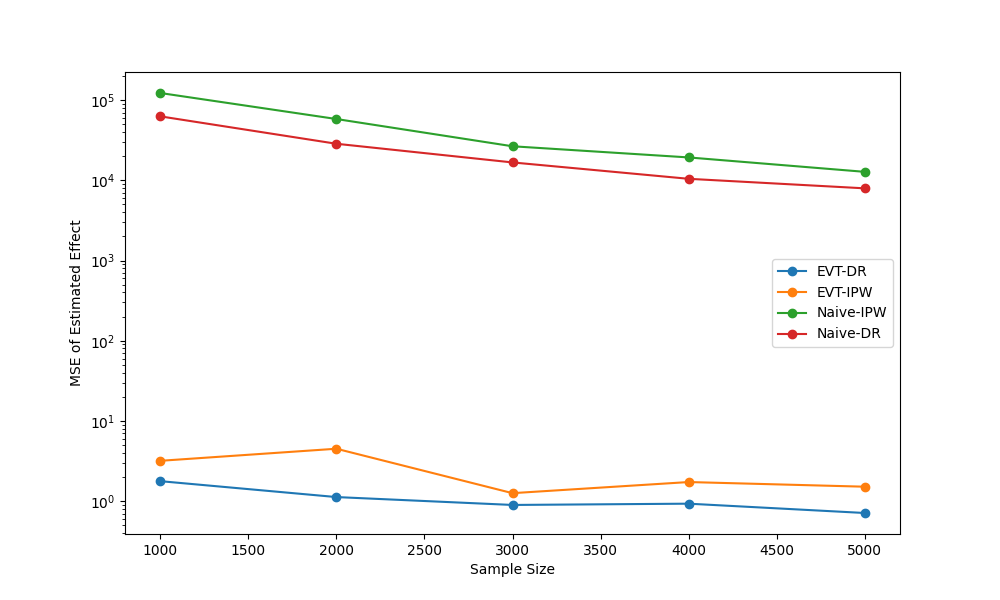
\includegraphics[width=\linewidth]{synthetic_experiment_pareto_20250515_50_1.5_1_10_50_1.0_adaptive__1000,_2000,_3000,_4000,_5000__othres.png}
  \end{minipage}
  \hfill
  \begin{minipage}[b]{0.45\textwidth}
    \centering
    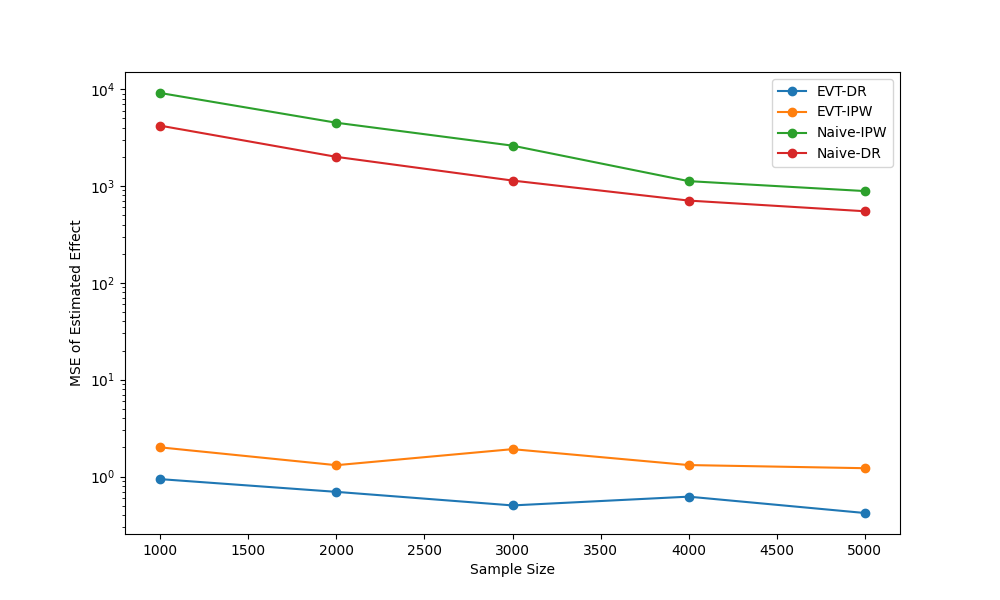
\includegraphics[width=\linewidth]{synthetic_experiment_pareto_20250515_50_1.5_1_5_30_1.0_adaptive__1000,_2000,_3000,_4000,_5000__othres.png}
  \end{minipage}
  \vspace{1em} % vertical separation
  % Second row
  \begin{minipage}[b]{0.45\textwidth}
    \centering
    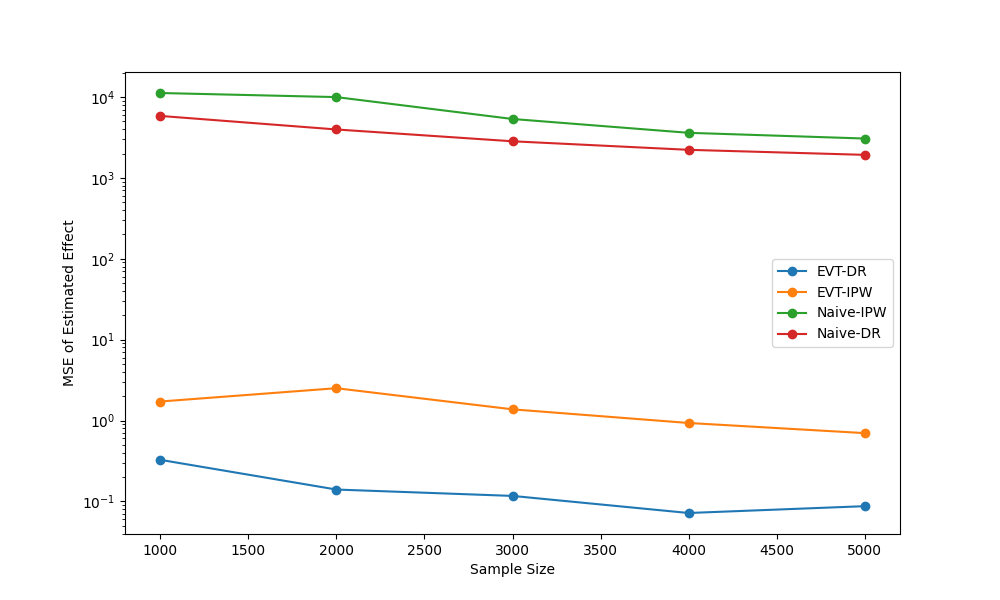
\includegraphics[width=\linewidth]{synthetic_experiment_pareto_20250515_50_2.5_1_5_30_1.0_adaptive__1000,_2000,_3000,_4000,_5000__othres.png}
  \end{minipage}
  \hfill
  \begin{minipage}[b]{0.45\textwidth}
    \centering
    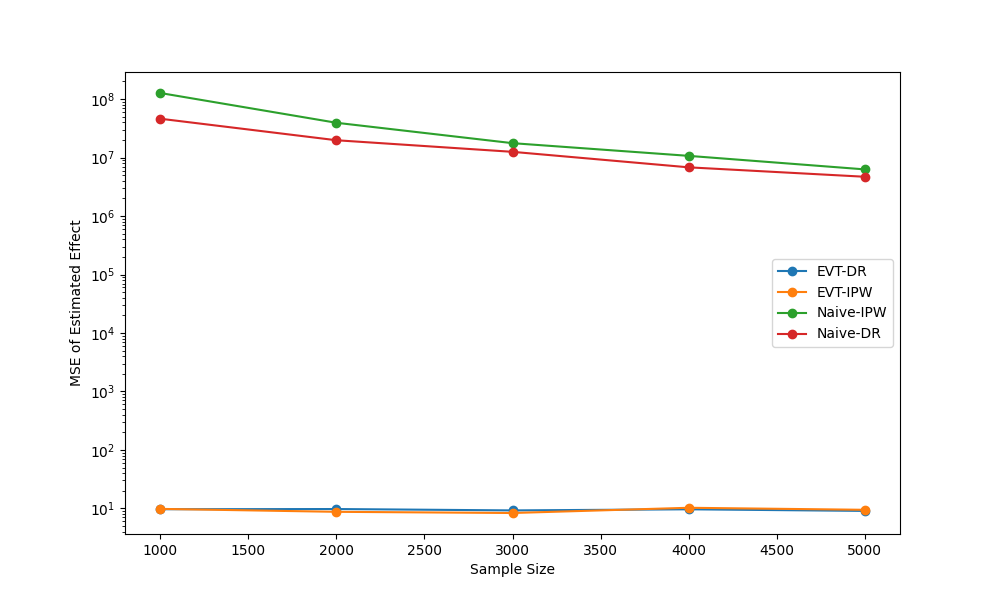
\includegraphics[width=\linewidth]{synthetic_experiment_pareto_20250516_50_2.5_2_5_30_1.0_adaptive__1000,_2000,_3000,_4000,_5000__othres.png}
  \end{minipage}

  \caption{Experiment results of four different configurations when the extreme noise is a linear transformation of Pareto variables. The configures of upper left, upper right, lower left and lower right are $ \alpha, \beta, d_z, d_u = (1, 1.5, 50, 10), (1, 1.5, 30, 5), (1, 2.5, 30, 5)$ and $ (2, 2.5, 30, 5)$ respectively. The results are averages of 50 repeated experiments. We use EVT-IPW and EVT-DR to represent $ \widehat{\theta}_{n,t}^{\mathrm{IPW}} $ and  $ \widehat{\theta}_{n,t}^{\mathrm{DR}} $ in \cref{alg:nete}.}
  \label{fig:synthetic}
\end{figure}

 Figure \ref{fig:synthetic} and \cref{fig:synthetic2} show that under different configurations of $\alpha,\beta, d_u, d_z$, our estimators generally perform better than the baseline estimators. The reason is that our estimators can make better use of the regularly varying structure. In general, EVT-DR achieves the smallest MSE in most experiments and is robust under different configurations. Note that the Pareto mixture does not satisfy \cref{assump:mvary}. \cref{fig:synthetic2} shows that our method still maintain a good performance even if \cref{assump:mvary} is violated. We also observe that sometimes the MSE increases with more samples in \cref{fig:synthetic2}. An explanation for this is that violation of \cref{assump:mvary} causes the threshold selection rule in \cref{cor:rate} not to be applicable and the variance term dominates the error.  
 
 %In some cases, the MSE is not decreasing when we increase the sample size, which can be caused by the fact that the biased term $e(t)$ dominates statistical error in \cref{cor:rate}.

\begin{figure}[!htbp]
  \centering
  % First row
  \begin{minipage}[b]{0.45\textwidth}
    \centering
    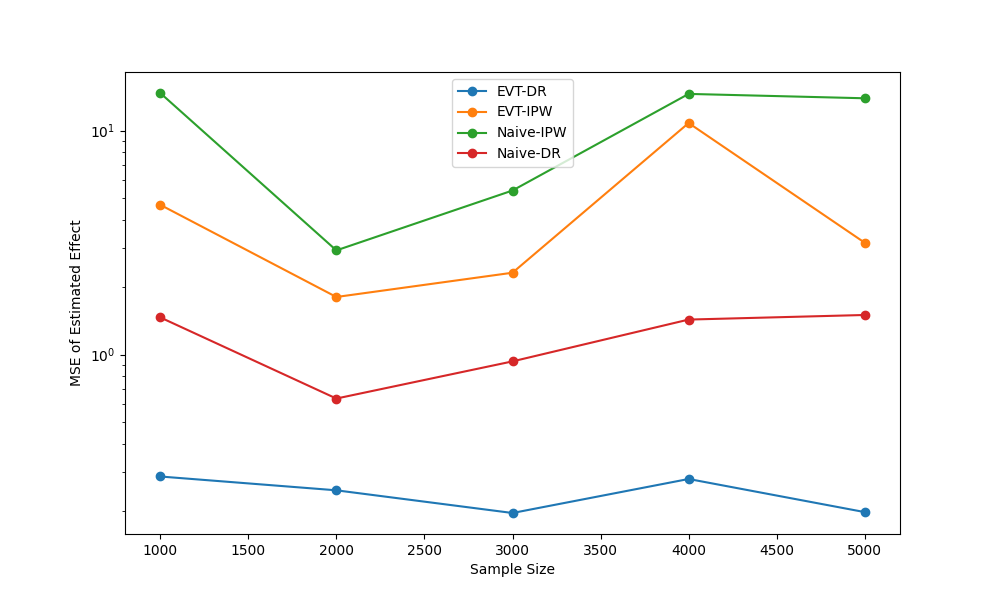
\includegraphics[width=\linewidth]{synthetic_experiment_pareto_mixture_20250515_50_1.5_1_10_50_1.0_adaptive__1000,_2000,_3000,_4000,_5000__othres.png}
  \end{minipage}
  \hfill
  \begin{minipage}[b]{0.45\textwidth}
    \centering
    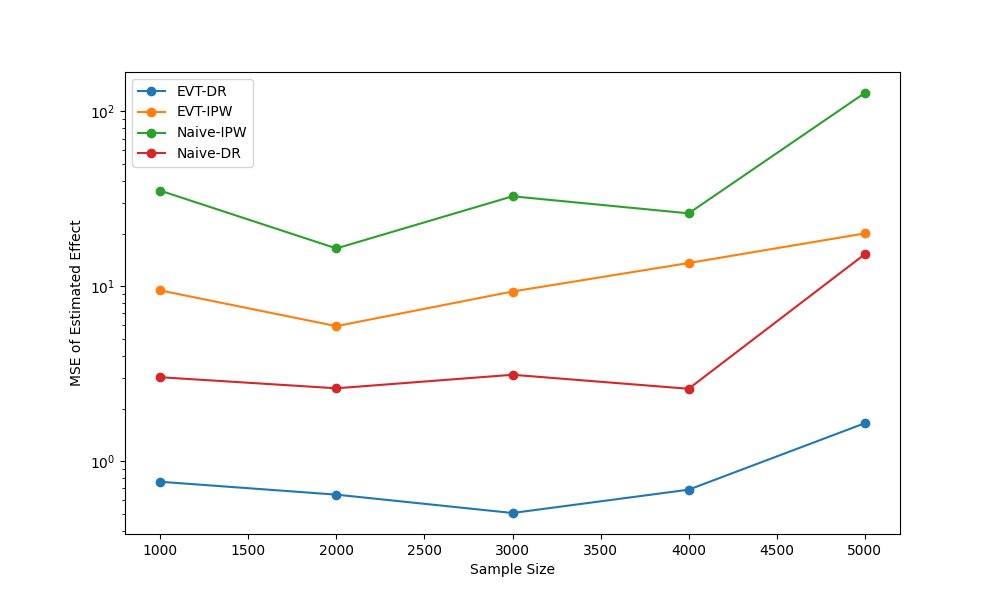
\includegraphics[width=\linewidth]{synthetic_experiment_pareto_mixture_20250515_50_1.5_1_5_30_1.0_adaptive__1000,_2000,_3000,_4000,_5000__othres.png}
  \end{minipage}
  \vspace{1em} % vertical separation
  % Second row
  \begin{minipage}[b]{0.45\textwidth}
    \centering
    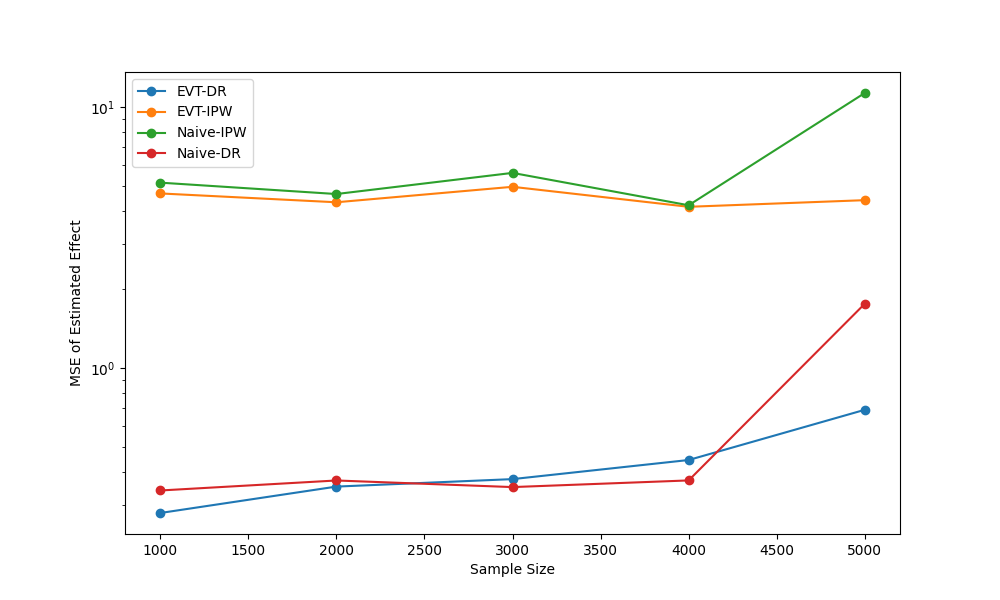
\includegraphics[width=\linewidth]{synthetic_experiment_pareto_mixture_20250515_50_2.5_1_5_30_1.0_adaptive__1000,_2000,_3000,_4000,_5000__othres.png}
  \end{minipage}
  \hfill
  \begin{minipage}[b]{0.45\textwidth}
    \centering
    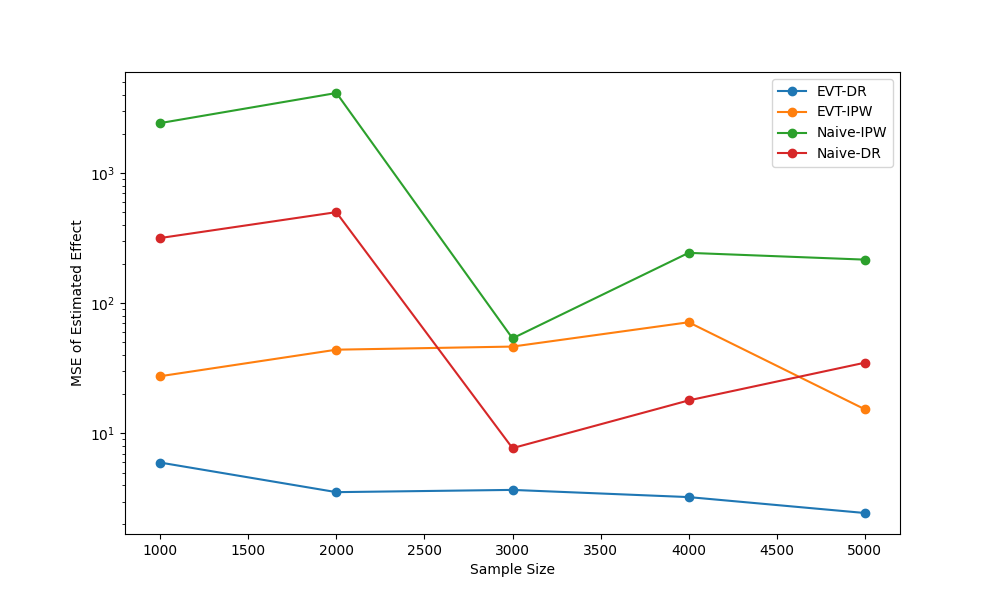
\includegraphics[width=\linewidth]{synthetic_experiment_pareto_mixture_20250515_50_2.5_2_5_30_1.0_adaptive__1000,_2000,_3000,_4000,_5000__othres.png}
  \end{minipage}

  \caption{Experiment results of four different configurations when the extreme noise is a Pareto mixture. The configures of upper left, upper right, lower left and lower right are $ \alpha, \beta, d_u = (1, 1.5, 10), (1, 1.5, 5), (1, 2.5,  5)$ and $ (2, 2.5, 5)$ respectively. The results are averages of 50 repeated experiments.}
  \label{fig:synthetic2}
\end{figure}
 

\subsection{Semi-synthetic Dataset}\label{subsec:semisyn}

Now, we use the wavesurge dataset \cite{coles2001introduction} to create a semi-synthetic dataset for our experiments. The wavesurge dataset has 2894 data points, which contain wave and surge heights at a single location off south-west England. Since wave and surge heights are not in the same scale and may not be positive, we shift the data and normalize each dimension by its $ 10 \% $ quantile. Given the wavesurget dataset, we generate our semi-synthetic dataset in the following way. 
\begin{align}
    & X \sim \text{Unif}(0,1), D \sim \text{Ber}(p(X)), \text{where} \  p(x) = 1/(1 + \exp(-x^\mathsf{T} b)), \notag\\
    & Y = (1 -  X + D)W^{\alpha_1} S^{\alpha_2} +  N(0,1), \label{eq:semi_syn}
\end{align}
where $ W $ and $ S $ are the height of the wave and surge, respectively. In this experiment, we evaluate how well our proposed EVT‑based estimators recover the Normalized Extreme Treatment Effect (NETE) when only limited “short‑term” data are available. We split the dataset into a training set (1,000 observations) and a test set (1,894 observations). First, we estimate the NETE on the training set using four estimators. Next, we apply the identification formula from Proposition \ref{prop:id} together with (\ref{eq:semi_syn}) to obtain a high‑fidelity estimate of the NETE on the test set. Because the test‑set estimate leverages additional data and the correct tail model, we treat it as a surrogate “ground truth” for comparison.  The real-world implications of this experiment is that we can use some short-term data (the training set) to predict long-term and unobserved behavior (the test set). 

\cref{tab:semi-synthetic} shows the results we get using different estimators. The results show that our EVT-IPW and EVT-DR give estimations that are closer to the test-set estimate than the naive estimators. In particular, the naive estimators consistently overshoot the true NETE by an order of magnitude. In addition, while more extreme tail configurations (e.g.\ $(1,3)$) slightly increase variance, the EVT‑based methods remain stable, with EVT‑DR deviating by at most 0.3 from the test‑set estimate.  These findings demonstrate that incorporating multivariate extreme value structure via our EVT‑IPW and EVT‑DR estimators substantially improves finite‑sample estimation of treatment effects on rare, tail events, compared both to naive methods. 

\begin{table}[!ht]
  \centering
  \caption{Causal Effect Estimates}
  \label{tab:semi-synthetic}
  \begin{tabular}{@{}cccccc@{}}
    \toprule
    $(\alpha_1, \alpha_2) $ & EVT-DR & EVT-IPW & Naive-DR  & Naive-IPW&  Test‐set Estimate \\
    \midrule
     (2, 2) & 0.18 &  0.25& 41.93  & 27.34  & 0.13 \\ 
     (1, 3) & 0.43 & 0.44 & 17.04 & 15.68  &0.13 \\
     (2.5, 1) & 0.13 & 0.18  & 31.64 & 26.06 & 0.20\\
     (1.5, 1.5) & 0.26 & 0.23 & 7.91 & 9.46  & 0.20\\
    \bottomrule
  \end{tabular}
\end{table}
 
\section{Conclusion}
In this paper, we addressed the challenge of estimating treatment effects on rare, high‐impact events by uniting tools from causal inference and extreme value theory. We introduced a new estimand that explicitly captures how an intervention shifts the tail average of the outcome distribution. Exploiting the spectral–magnitude decomposition inherent in multivariate regular variation, we obtained a simple, implementable identification formula (Proposition \ref{prop:id}). Building on this, we constructed both inverse‐propensity‐weighted (IPW) and doubly‐robust (DR) estimators, and we further established non‐asymptotic error bounds under a Pareto‐type tail assumption (\cref{thm:rate}, \cref{cor:rate}). In simulations and real‐data experiments, our methods consistently outperformed naive estimators when targeting extreme outcomes, thereby validating our theoretical guarantees. We believe this work opens the door to more refined causal analyses in applications—such as disaster risk reduction and financial risk management—where understanding treatment effects in the tail is paramount. One limitation of this work is that we mainly use heuristics to estimate the scaling exponential $\alpha $, which lacks a theoretical guarantee. For future direction, we would like to explore how to estimate the exponential $\alpha$ and develop a more adaptive method for choosing thresholds for our estimators. 

\bibliography{reference}
\bibliographystyle{plainnat}

\newpage

\appendix
 

\section{Proofs}
\subsection{Identification Formula}
In this subsection, we derive the identification formula in Proposition
\ref{prop:id}.

\begin{proof}
Write $R_U=\|U\|$, $S_U=U/\|U\|$, and $\bar e(t)=\sup_{r\geq t}e(r)$; the last quantity is finite for sufficiently large $t$ and tends to zero. Independence of $U$ from $(X,D)$ gives $\mathbb P(D=1\mid X,U)=p(X)$. Positivity, consistency, and conditional mean exogeneity given $(X,U)$ therefore give, for both treatments, 
\[
f(X,d,U)=\mathbb E[Y(d)\mid X,U,D=d]=\mathbb E[Y(d)\mid X,U].
\]
 The assumed absolute tail means justify taking conditional expectations on $\{R_U>t\}$. Homogeneity at the realized radius yields 
\[
\frac{f(X,1,U)-f(X,0,U)}{R_U^{\alpha}}=g(X,1,S_U)-g(X,0,S_U)+\varepsilon(X,U),\qquad |\varepsilon(X,U)|\leq2\bar e(t)\quad\hbox{on }\{R_U>t\}.
\]
 Consequently, 
\[
\left|\mathbb E\left[\frac{Y(1)-Y(0)}{t^{\alpha}}\mid R_U>t\right]-\mathbb E\left[(g(X,1,S_U)-g(X,0,S_U))(R_U/t)^{\alpha}\mid R_U>t\right]\right|\leq2\bar e(t)\mathbb E[(R_U/t)^{\alpha}\mid R_U>t].
\]
 We next establish that the radial moment tends to $\beta/(\beta-\alpha)$. For every real $a<\beta$, the identity $x^a=1+\int_1^x a r^{a-1}\,\tmop{dr}$, together with absolute integrability of the integral, gives 
\[
\mathbb E[(R_U/t)^a\mid R_U>t]=1+\int_1^{\infty}a r^{a-1}\frac{\mathbb P(R_U>tr)}{\mathbb P(R_U>t)}\,\tmop{dr}.
\]
 For $a=0$ the integral is zero; for $a<0$ its absolute integrability follows from $\int_1^{\infty}|a|r^{a-1}\,\tmop{dr}=1$.

Note that $\| U \|$ is also regularly varying. By Potter's theorem \cite[Theorem 1.56]{bingham1989regular}, for any $\epsilon >0$ and sufficiently large $t$, we have
\begin{align*}
  \frac{P (\| U \| > {rt})}{P (\| U \| > t)} & \leqslant 2 r^{-\beta + \epsilon} .
\end{align*}

For $0<a<\beta$, choose $0<\epsilon<\beta-a$. The Potter bound dominates the absolute integrand by $2a r^{a-\beta+\epsilon-1}$, whose integral is finite. For $a<0$, the bound by $|a|r^{a-1}$ also permits dominated convergence. Regular variation thus gives, for every $a<\beta$, 
\[
\mathbb E[(R_U/t)^a\mid R_U>t]\longrightarrow1+\int_1^{\infty}a r^{a-\beta-1}\,\tmop{dr}=\frac{\beta}{\beta-a}.
\]
 In particular, the radial moments with $a=\alpha$ are bounded, and the preceding homogeneity error tends to zero. Define 
\[
G(s)=\mathbb E_X[g(X,1,s)-g(X,0,s)],\qquad h_t(r,s)=G(s)r^{\alpha}.
\]
 Independence of $X$ and $U$ shows that the remaining conditional expectation is $\mathbb E[h_t(R_U/t,S_U)\mid R_U>t]$.
Note that by Assumption \ref{assump:f_homo}, $g$ is a continuous function on a
compact set and thus is bounded by some constant $C > 0$. Thus $|G(s)|\leq2C$, and $G$ is continuous. If $\alpha\leq0$, then $|h_t(r,s)|\leq2C$ for $r\geq1$. If $\alpha>0$, choose $p>1$ with $p\alpha<\beta$. The radial moment calculation gives 
\[
\sup_{t\geq t_0}\mathbb E[|G(S_U)(R_U/t)^{\alpha}|^p\mid R_U>t]\leq(2C)^p\sup_{t\geq t_0}\mathbb E[(R_U/t)^{p\alpha}\mid R_U>t]<\infty.
\]
 This establishes uniform integrability in both cases. Definition~\ref{def:mvarying} gives conditional weak convergence of $(R_U/t,S_U)$ to the product of a Pareto radial law with survival $r^{-\beta}$ for $r\geq1$ and the spectral probability measure $S$. For a bounded truncation of $G(s)r^{\alpha}$, weak convergence gives convergence of expectations. Uniform integrability makes the truncation errors tend to zero uniformly, so 
\[
\lim_{t\rightarrow\infty}\mathbb E[G(S_U)(R_U/t)^{\alpha}\mid R_U>t]=\left(\int G(s)\,S(\tmop{ds})\right)\frac{\beta}{\beta-\alpha}.
\]
 Weak convergence of the angular marginal and bounded continuity of $G$ also give 
\[
\lim_{t\rightarrow\infty}\mathbb E[g(X,1,S_U)-g(X,0,S_U)\mid R_U>t]=\int G(s)\,S(\tmop{ds}).
\]
 Combining these two limits with the vanishing homogeneity error proves the stated product formula.
\end{proof}

\subsection{Non-asymptotic Analysis}

To obtain a convergence rate for the estimator $\hat{\theta}_n^t$, we first analyze the rate of the two factors $\hat{\gamma}_n$ and $\hat{\eta}_{n,t}^{\text{DR}}$.

\begin{lemma}
  \label{lemma:mu_rate} Under Assumption \ref{assump:iid}, \ref{assump:mvary}, using the standing convention $\|\cdot\|=\|\cdot\|_1$, let $R_i=\|U_i\|_1$ for all $i\in\{1,\ldots,n\}$ and order these full-input radii as $R_{[1]}\geq\cdots\geq R_{[n]}$. For $n\geq2$, define

\[
H_n(k)=\frac1k\sum_{j=1}^k\log\frac{R_{[j]}}{R_{[k+1]}},\qquad 1\leq k\leq n-1.
\]

For $\delta\in(0,1)$, set

\[
\begin{aligned}
L_n&=\min\{n-1,\lceil100\log n\rceil\},&J_n&=1+\lceil\log n/\log2\rceil,\\
q_n(\delta)&=\log(4J_n/\delta),&c_n(\delta)&=2\sqrt{q_n(\delta)}+\frac{q_n(\delta)}{\sqrt{L_n}},\\
\rho_n(\delta)&=16c_n(\delta).
\end{aligned}
\]

Let

\[
\begin{aligned}
\widetilde k_n&=\max\bigl\{k\in\{L_n,\ldots,n-1\}:\\
&\qquad |H_n(i)-H_n(k)|\leq\frac{H_n(i)\rho_n(\delta)}{\sqrt i}\\
&\qquad \text{for every }i\in\{L_n,\ldots,k\}\bigr\},\\
\widetilde\gamma_n&=H_n(\widetilde k_n).
\end{aligned}
\]

For each fixed $\delta\in(0,1)$ and every sufficiently large $n$, with probability at least $1-\delta$, we have

\[
|\gamma-\widetilde\gamma_n|\leq C_\delta
\begin{cases}
\left(\dfrac{\log((8/\delta)\log n)}{n}\right)^{1/3},&0<\beta<1,\\
\left(\dfrac{\log n\,\log((8/\delta)\log n)}{n}\right)^{1/3},&\beta=1,\\
\left(\dfrac{\log((8/\delta)\log n)}{n}\right)^{1/(2+\beta)},&\beta>1,
\end{cases}
\]

where $C_\delta$ may depend on the fixed distribution and on $\delta$.
  
  where $\gamma = 1 / \beta$ is the EVI of $U$. 
\end{lemma}

\noindent\textit{Remark.} For each fixed $\delta\in(0,1)$ there is a deterministic $n_0$ such that, for every integer $n\geq n_0$, the bound has probability at least $1-\delta$ under the law of the sample of size $n$.

\begin{proof}
  We adopt the non-asymptotic analysis of the adaptive Hill estimator for EVI
  in {\citep{boucheron2015tail}}. We give the exponential-spacing argument and the confidence calibration explicitly. Write $R=\|U\|_1$. Fix a member of $M_K$, put $a_i=\|A_{\cdot i}\|_1$, and let $Z_i^0$ be independent nominal Pareto type-II components of index $\beta$. The component density is a positive constant $c_0$ times the nominal product density whenever $\|z\|_1>\zeta K^{(1-2s)/\beta}$. Since

\[
R=\sum_{i=1}^m a_iZ_i,\qquad l\leq a_i\leq u,\qquad R\leq u\|Z\|_1,
\]

the survival and density of $R$ beyond $u\zeta K^{(1-2s)/\beta}$ are $c_0$ times those of $T=\sum_i a_iZ_i^0$. This transfer uses the original nominal components without shifting their supports. 

Put $W_i=a_iZ_i^0$, $V_i=\sum_{j\ne i}W_j$, and $f_i(x)=\beta a_i^\beta(a_i+x)^{-\beta-1}$ for $x\geq0$, extended by zero for $x<0$. Partitioning the convolution integral according to the largest summand, whose ties have probability zero, gives

\[
f_T(r)=\sum_i\mathbb E\left[f_i(r-V_i)I\{\max_{j\ne i}W_j\leq r-V_i\}\right].
\]

On this event $r-V_i\geq r/m$. If $V_i\leq r/2$, the event holds and the mean value theorem gives $|f_i(r-V_i)-f_i(r)|\leq C r^{-\beta-2}V_i$. On the part where $V_i>r/2$, the indicated density is at most $C r^{-\beta-1}$. A union bound using the tails of the $m-1$ summands gives $\mathbb P(V_i>x)\leq Cx^{-\beta}$ for $x\geq1$. Integrating this bound and using $\mathbb E[V_iI\{V_i\leq r/2\}]\leq\mathbb E[\min\{V_i,r/2\}]$ gives

\[
\mathbb E[V_iI\{V_i\leq r/2\}]\leq
\begin{cases}Cr^{1-\beta},&\beta<1,\\ C\log r,&\beta=1,\\ C,&\beta>1.\end{cases}
\]

Consequently

\[
\left|f_T(r)-\sum_i f_i(r)\right|
\leq C\sum_i\left(r^{-\beta-2}\mathbb E[V_iI\{V_i\leq r/2\}]+r^{-\beta-1}\mathbb P(V_i>r/2)\right).
\]

Since $\sum_i f_i(r)=\beta\sum_i a_i^\beta r^{-\beta-1}(1+O(r^{-1}))$, set

\[
b_\beta(r)=\begin{cases}r^{-\beta},&\beta<1,\\r^{-1}\log r,&\beta=1,\\r^{-1},&\beta>1,\end{cases}\qquad C_0=c_0\sum_i a_i^\beta>0.
\]

The actual radial density and survival therefore satisfy, for sufficiently large $r$,

\[
f_R(r)=\beta C_0r^{-\beta-1}(1+O(b_\beta(r))),\qquad
\bar F_R(r)=C_0r^{-\beta}(1+O(b_\beta(r))).
\]

The second estimate follows by integrating the first error from $r$ to infinity: the integrals of $r^{-2\beta-1}$, $r^{-3}\log r$, and $r^{-\beta-2}$ have orders $r^{-2\beta}$, $r^{-2}\log r$, and $r^{-\beta-1}$, respectively. Thus no constant-coefficient expansion at $\beta=1$ is required. When $\beta>1$ and a survival expansion with coefficient $D$ is used, differentiation gives density coefficient $D(1+1/\beta)$; the density and survival envelopes just proved avoid differentiating an unspecified remainder. 

Let $Q(v)=F_R^{-1}(1-1/v)$ be the radial tail quantile. Its differentiable tail has $Q(v)\sim(C_0v)^{1/\beta}$ and

\[
\eta(v)=\frac{vQ'(v)}{Q(v)}-\gamma
=\frac{\bar F_R(Q(v))}{Q(v)f_R(Q(v))}-\frac1\beta
=O(b_\beta(Q(v))).
\]

Choose a fixed $v_0>1$ in that tail and define $\bar\eta(v)=\sup_{w\geq\max\{v,v_0\}}|\eta(w)|$ for every $v>0$. For sufficiently large $v$ this gives

\[
\bar\eta(v)\leq
\begin{cases}Cv^{-1},&\beta<1,\\Cv^{-1}\log v,&\beta=1,\\Cv^{-1/\beta},&\beta>1.\end{cases}
\]

For $y\geq z\geq\log v_0$, integrating the quantile derivative gives

\[
|\log Q(e^y)-\log Q(e^z)-\gamma(y-z)|\leq\bar\eta(e^z)(y-z).
\]
 

We next prove the simultaneous stochastic bound used for selection. Let $Y_{(1)}\geq\cdots\geq Y_{(n)}$ be decreasing order statistics of independent standard exponential variables, with $Y_{(n+1)}=0$. Their joint density is $n!\exp(-\sum_j y_j)$ on the ordered region. The change of variables $E_j=j(Y_{(j)}-Y_{(j+1)})$ has Jacobian $1/n!$ and $\sum_j y_j=\sum_j E_j$, so the $E_j$ are independent standard exponential variables. The quantile transform represents the ordered radii as $Q(e^{Y_{(j)}})$. Define $B_i=\sum_{j=1}^i(E_j-1)$ and $A_i=i^{-1}\sum_{j=1}^iE_j$ for this argument only. 

For $0<\lambda<1$,

\[
\log\mathbb E e^{\lambda(E_j-1)}=-\lambda-\log(1-\lambda)\leq\frac{\lambda^2}{2(1-\lambda)},\qquad
\log\mathbb E e^{-\lambda(E_j-1)}=\lambda-\log(1+\lambda)\leq\frac{\lambda^2}{2(1-\lambda)}.
\]

Hence $\exp(\pm\lambda B_i-i\lambda^2/(2(1-\lambda)))$ are nonnegative supermartingales with initial value one. The maximal supermartingale inequality implies

\[
\mathbb P\left(\max_{i\leq m}|B_i|\geq\sqrt{2mx}+x\right)\leq2e^{-x}.
\]

Indeed, each one-sided probability is at most $\exp(-\lambda a+m\lambda^2/(2(1-\lambda)))$ for $a=\sqrt{2mx}+x$; taking $\lambda=\sqrt{2x/m}/(1+\sqrt{2x/m})$ makes this bound $e^{-x}$. 

Apply this inequality at the ends of the dyadic intervals $2^a\leq i<2^{a+1}$, using $m=\min\{n,2^{a+1}\}$ and $x=q_n(\delta)$. There are at most $J_n$ such intervals. On each interval $\sqrt{2m}/\sqrt i\leq2$. The union bound therefore supplies an event $E$ of probability at least $1-\delta/2$ on which

\[
\sqrt i\,|A_i-1|\leq2\sqrt{q_n(\delta)}+q_n(\delta)/\sqrt i\leq c_n(\delta),\qquad L_n\leq i\leq n.
\]

For fixed $\delta$, $c_n(\delta)=O_\delta(\sqrt{\log\log n})$ and $c_n(\delta)/\sqrt{L_n}\to0$. 

Write $c_n=c_n(\delta)$ and consider the deterministic index

\[
k_* =\max\left\{k\in\{L_n,\ldots,n-1\}:\ \frac{n}{2k}\geq v_0,\quad
\sqrt k\,\bar\eta\left(\frac{n}{2k}\right)\leq\gamma c_n\right\}.
\]

The choices below show that this set is nonempty for all sufficiently large $n$. Put $T_*=e^{Y_{(k_*+1)}}$. The number of exponential observations exceeding $\log(n/(2k_*))$ has binomial law with mean $2k_*$. Its multiplicative lower-tail bound gives

\[
\mathbb P\left(T_*<\frac{n}{2k_*}\right)\leq\exp(-k_*/4)\leq\delta/2
\]

for sufficiently large $n$, because $k_*\geq L_n$. Indeed, if $B\sim\tmop{Bin}(n,p)$ and $\mu=np$, Markov's inequality gives

\[
\mathbb P(B\leq\mu/2)\leq e^{\mu\log2/2}\mathbb E[2^{-B}]
=e^{\mu\log2/2}(1-p/2)^n
\leq e^{-\mu(1-\log2)/2}\leq e^{-\mu/8},
\]

using $\log2\leq3/4$; here $p=2k_*/n$ and $\mu=2k_*$. Let $E_*$ be the complementary event. On $E_*$ all spacings involved in $H_n(i)$ for $i\leq k_*$ lie above $\log v_0$. Since $H_n(i)=i^{-1}\sum_{j=1}^i j\log(R_{[j]}/R_{[j+1]})$ by telescoping, the quantile inequality thus gives

\[
|H_n(i)-\gamma A_i|\leq\bar\eta(T_*)A_i\leq\frac{\gamma c_n}{\sqrt{k_*}}A_i,\qquad L_n\leq i\leq k_*.
\]

On $E\cap E_*$, for large enough $n$, $c_n/\sqrt{L_n}\leq1/6$. It follows that

\[
|H_n(i)-\gamma|\leq\frac{\gamma c_n}{\sqrt i}+\frac{\gamma c_n}{\sqrt{k_*}}\left(1+\frac{c_n}{\sqrt i}\right)
\leq\frac{3\gamma c_n}{\sqrt i},\qquad
\gamma/2\leq H_n(i)\leq3\gamma/2.
\]

For every $L_n\leq i\leq k\leq k_*$,

\[
|H_n(i)-H_n(k)|\leq\frac{6\gamma c_n}{\sqrt i}
\leq\frac{H_n(i)\rho_n(\delta)}{\sqrt i}.
\]

Thus $k_*$ qualifies for the displayed prefix rule, and its selected index $\widetilde k_n$ is at least $k_*$. The set in that rule is nonempty almost surely because $k=L_n$ only compares with itself. The comparison at $i=k_*$ now yields

\[
|\widetilde\gamma_n-\gamma|\leq|H_n(k_*)-\gamma|+\frac{H_n(k_*)\rho_n(\delta)}{\sqrt{k_*}}
\leq\frac{27\gamma c_n}{\sqrt{k_*}}.
\]

The two events used have total failure probability at most $\delta$; independence between them is unnecessary. 

To obtain the displayed rates, when $\beta\ne1$ put $p=\min\{1,1/\beta\}$ and choose a sufficiently small fixed $a_*>0$. Let

\[
k_0=\left\lfloor a_* n^{2p/(1+2p)}c_n^{2/(1+2p)}\right\rfloor.
\]

For all sufficiently large $n$, $k_0\geq L_n$, $k_0<n/(2v_0)$, and

\[
\sqrt{k_0}\,\bar\eta(n/(2k_0))\leq C2^p k_0^{p+1/2}n^{-p}\leq\gamma c_n
\]

by making $a_*$ small. Thus $k_*\geq k_0$, and

\[
\frac{c_n}{\sqrt{k_*}}\leq C n^{-p/(1+2p)}c_n^{2p/(1+2p)}
\leq C_\delta\left(\frac{\log((8/\delta)\log n)}n\right)^{p/(1+2p)}.
\]

Here $c_n^2\leq C_\delta\log((8/\delta)\log n)$ for sufficiently large $n$. For $\beta<1$ the exponent is $1/3$, and for $\beta>1$ it is $1/(2+\beta)$. 

When $\beta=1$, take

\[
k_0=\left\lfloor a_*n^{2/3}\left(\frac{c_n}{\log n}\right)^{2/3}\right\rfloor.
\]

Again $k_0\geq L_n$ and $k_0<n/(2v_0)$ eventually, and

\[
\sqrt{k_0}\,\bar\eta(n/(2k_0))\leq Ck_0^{3/2}n^{-1}\log n\leq\gamma c_n
\]

for sufficiently small $a_*$. Hence $k_*\geq k_0$ and

\[
\frac{c_n}{\sqrt{k_*}}\leq C n^{-1/3}(c_n^2\log n)^{1/3}
\leq C_\delta\left(\frac{\log n\,\log((8/\delta)\log n)}n\right)^{1/3}.
\]

This proves the middle case on the same event of probability at least $1-\delta$, and completes the proof.
\end{proof}

\begin{lemma}
  \label{lemma:eta_rate} Under the assumption of Theorem \ref{thm:rate}, suppose in addition that the conditions of Proposition~\ref{prop:id} hold. Suppose that the fitted propensity, regression, and exponent are measurable with respect to the training split and independent auxiliary data. Suppose that the nuisance inequalities of Theorem~\ref{thm:rate} hold jointly with probability at least $1-\varepsilon$, uniformly almost surely over the covariate and direction support and both treatments, for each tolerance $\varepsilon$. Suppose that $0<p(X)<1$ almost surely and that the fitted-exponent pseudo-outcome has finite conditional absolute mean on those nuisance events. Put $\pi_t=\mathbb P(\|U\|>t)$ and $M=|\mathcal I|$, and set $\hat\eta_{n,t}^{\tmop{DR}}=0$ when $M=0$. Let $\bar e(t)=\sup_{r\geq t}e(r)$, let $C$ bound $|g|$ on its compact domain, and put $G_t=C+\bar e(t)$. For a generic evaluation observation define 
\[
\psi=\hat g(X,1,U/\|U\|)-\hat g(X,0,U/\|U\|)+\frac{D-\hat p(X)}{\hat p(X)(1-\hat p(X))}\left(\frac{Y}{\|U\|^{\hat\alpha_n}}-\hat g(X,D,U/\|U\|)\right).
\]
 For any positive truncation level $B$ chosen using only the training split and independent auxiliary data, define 
\[
\begin{aligned} v_t(B)&=\mathbb E[\psi^2 I\{|\psi|\leq B\}\mid\mathcal D_1,\hbox{ auxiliary data},\|U\|>t],\\ a_t(B)&=\mathbb E[|\psi|I\{|\psi|>B\}\mid\mathcal D_1,\hbox{ auxiliary data},\|U\|>t]. \end{aligned}
\]
 Fix $a_0\in(0,\beta)$ and write $a=R_\alpha(n,\delta/4)$. For sufficiently large $t\geq1$, if $a\leq a_0$ and $n\pi_t\geq16\log(4/\delta)$, then with probability at least $1-\delta$ we have $M\geq n\pi_t/4$ and \begin{align*} |\hat\eta_{n,t}^{\tmop{DR}}-\eta|\leq{}&\sqrt{\frac{4v_t(B)}{\delta M}}+\left(1+\frac4\delta\right)a_t(B)+\frac2c R_p(n/2,\delta/4)R_g(n_t,\delta/4)\\ &+2\bar e(t)+2L W_1(\mathcal L_{U/\|U\|}^t,\mathcal L_{U/\|U\|})+\frac{2G_t}{c}\left(t^a-1+K a t^a\right), \end{align*} where $K$ depends on the radial law and $a_0$. Suppose moreover that the angular Wasserstein term satisfies the bound that Proposition 3.1 of \citet{zhang2023wasserstein} gives for this Pareto-type model, which is taken from that work and not proved here: there are constants $C_W>0$, $k\geq0$ and $t_W\geq1$ such that 
\[
W_1(\mathcal L_{U/\|U\|}^t,\mathcal L_{U/\|U\|})\leq C_W(\log t)^k t^{-\min\{1,\beta\}}+C_W t^{-\beta s/(1-2s)}\qquad(t\geq t_W).
\]
 Then for $t\geq t_W$ the angular term $2L W_1(\mathcal L_{U/\|U\|}^t,\mathcal L_{U/\|U\|})$ of the display is at most $2LC_W(\log t)^k t^{-\min\{1,\beta\}}+2LC_W t^{-\beta s/(1-2s)}$, with the logarithmic factor retained. When the conditional score variance $V_t$ is finite, the sampling term may instead be taken to be $\sqrt{4V_t/(\delta M)}$.
\end{lemma}

\noindent\textit{Remark.} Assumption~\ref{assump:mvary} specifies the noise law $\mathcal L(U)$. The component dimension in the density of Assumption~\ref{assump:mvary} is $m=d_z$. The equal split in Algorithm~\ref{alg:nete} is defined for positive even sample sizes $n$, with $|\mathcal D_1|=|\mathcal D_2|=n/2$. The sample-size domain of $R_g(q,\varepsilon)$ includes every possible training exceedance count $q\in\{0,1,\ldots,n/2\}$, including $q=0$. The target $\eta$ denotes $\int\mathbb E_X[g(X,1,s)-g(X,0,s)]\,S(\tmop{ds})$, where $S$ is the limiting spectral probability measure. The symbol $V_t$ denotes $\tmop{Var}(\psi\mid\mathcal D_1,\hbox{ auxiliary data},\|U\|>t)$. The homogeneity inequality holds for both treatments and every positive radius, on the positive unit sphere for the $\ell_1$ norm. The fitted-exponent pseudo-outcome has finite conditional absolute mean under the evaluation tail law: $\mathbb E[|Y|/\|U\|^{\hat\alpha_n}\mid\mathcal D_1,\hbox{ auxiliary data},\|U\|>t]<\infty$ almost surely on each joint nuisance event.

\noindent\textit{Remark (notation).} $\hat\eta_{n,t}^{\tmop{DR}}$ is the average normalized doubly robust score over exceedances in the second half $\mathcal{D}_2$, using $\hat p$ and $\hat g$ fitted on the first half $\mathcal{D}_1$ and the supplied exponent $\hat\alpha_n$, wherever $|\mathcal{I}|>0$. In Lemma~\ref{lemma:eta_rate}: Set $\hat\eta_{n,t}^{\tmop{DR}}=0$ when $M=|\mathcal I|=0$; conditional on $\mathcal D_1$ and the independent auxiliary data, the fitted $\hat p$, $\hat g$, and $\hat\alpha_n$ are fixed, and for $M>0$ the estimator averages the displayed score $\psi$ over the evaluation exceedances. In Corollary~\ref{cor:rate}: The estimator is evaluated at $t_n=\Theta(n^{(1-2s)\hat\gamma_n})$ in the first item and $t_n=\Theta(n^{\hat\gamma_n/(1+2\min\{1,\hat\gamma_n\})})$ in the second item, with deterministic positive order constants independent of $n$ and the sample. Set $\hat\eta_{n,t}^{\tmop{DR}}=0$ when there are no evaluation exceedances. The fitted $\hat p$, $\hat g$, and $\hat\alpha_n$ are $\mathcal T$-measurable, where $\mathcal T$ consists of the training split and independent auxiliary data, and are the same functions and exponent for every input threshold; they are held fixed in the score moments conditional on $\mathcal T$ and $\|U\|>t$. In Theorem~\ref{thm:rate}: Set $\hat\eta_{n,t}^{\tmop{DR}}=0$ when $M=|\mathcal I|=0$; conditional on the training split and independent auxiliary data $\mathcal T$, the fitted $\hat p$, $\hat g$, and $\hat\alpha_n$ are fixed, and for $M>0$ the estimator averages $\psi^{\mathrm{DR}}$ over the evaluation exceedances. In Lemma~\ref{lemma:eta_ipw}: Set $\hat\eta_{n,t}^{\tmop{DR}}=0$ when $M=|\mathcal I|=0$; conditional on the training split and independent auxiliary data $\mathcal T$, the fitted $\hat p$, $\hat g$, and $\hat\alpha_n$ are fixed, and for $M>0$ the estimator averages the normalized doubly robust score over the evaluation exceedances.

\begin{proof}
Condition on the training split and independent auxiliary data, denoted together by $\mathcal T$. Write $R_U=\|U\|$, $S_U=U/\|U\|$, and 
\[
m_d^t(x,s)=\mathbb E[Y/R_U^{\alpha}\mid X=x,D=d,S_U=s,R_U>t],\qquad \eta_\alpha^t=\mathbb E[(f(X,1,U)-f(X,0,U))/R_U^{\alpha}\mid R_U>t].
\]
 Independence of $U$ from $(X,D)$ gives $\mathbb E[D\mid X,S_U,R_U>t]=p(X)$. Let $\psi_\alpha$ be the score $\psi$ with $\hat\alpha_n$ replaced by $\alpha$, keeping the same fitted functions. Direct conditional expectation over treatment and outcome gives \begin{align*} \mathbb E[\psi_\alpha\mid\mathcal T,R_U>t]-\eta_\alpha^t=\mathbb E\left[(p(X)-\hat p(X))\left\{\frac{m_1^t(X,S_U)-\hat g(X,1,S_U)}{\hat p(X)}+\frac{m_0^t(X,S_U)-\hat g(X,0,S_U)}{1-\hat p(X)}\right\}\mid\mathcal T,R_U>t\right]. \end{align*} Indeed, the coefficients of $m_1^t-\hat g_1$ and $m_0^t-\hat g_0$ are respectively $p/\hat p-1$ and $1-(1-p)/(1-\hat p)$, which equal $(p-\hat p)/\hat p$ and $(p-\hat p)/(1-\hat p)$. On the joint nuisance event at tolerance $\delta/4$, the uniform bounds and estimated-propensity overlap therefore imply 
\[
|\mathbb E[\psi_\alpha\mid\mathcal T,R_U>t]-\eta_\alpha^t|\leq\frac2c R_p(n/2,\delta/4)R_g(n_t,\delta/4).
\]
  
  where $n_t = \sum_{i = 1}^{n/2} I (\|U_i \|> t)$ is a random variable. Keep this training count as the argument of $R_g$; no regularity of that error function beyond its stated monotonicity is needed. Homogeneity at each realized radius gives 
\[
|\eta_\alpha^t-\mathbb E[g(X,1,S_U)-g(X,0,S_U)\mid R_U>t]|\leq2\bar e(t).
\]
 The function $s\mapsto\mathbb E_X[g(X,1,s)-g(X,0,s)]$ is $2L$-Lipschitz. Independence of $X$ and $U$ and the definition of the limiting angular target therefore give 
\[
|\eta_\alpha^t-\eta|\leq2\bar e(t)+2L W_1(\mathcal L_{U/\|U\|}^t,\mathcal L_{U/\|U\|}).
\]
 Proposition 3.1 of \cite{zhang2023wasserstein}, with Wasserstein order one and tail index $\beta$, supplies the stated angular bound with its logarithmic factors. Next, the fitted functions cancel from $\psi-\psi_\alpha$. Taking conditional expectation over the outcome and treatment leaves 
\[
\mathbb E\left[\left\{\frac{p(X)}{\hat p(X)}\frac{f(X,1,U)}{R_U^{\alpha}}-\frac{1-p(X)}{1-\hat p(X)}\frac{f(X,0,U)}{R_U^{\alpha}}\right\}\left(R_U^{\alpha-\hat\alpha_n}-1\right)\mid\mathcal T,R_U>t\right].
\]
 On the nuisance event, $|\alpha-\hat\alpha_n|\leq a$. Since $R_U\geq t\geq1$, we have $|R_U^{\alpha-\hat\alpha_n}-1|\leq R_U^a-1$. Homogeneity also gives $|f(X,d,U)/R_U^{\alpha}|\leq G_t$, so 
\[
|\mathbb E[\psi-\psi_\alpha\mid\mathcal T,R_U>t]|\leq\frac{2G_t}{c}\mathbb E[R_U^a-1\mid R_U>t].
\]
 Choose $\epsilon=(\beta-a_0)/2>0$. Potter's bound gives, uniformly for $r\geq1$ and sufficiently large $t$, 
\[
\frac{\mathbb P(R_U>tr)}{\pi_t}\leq2r^{-\beta+\epsilon}.
\]
 Integrating the radial tail, for $0\leq a\leq a_0$, yields \begin{align*} \mathbb E[R_U^a-1\mid R_U>t]&=t^a-1+t^a\int_1^{\infty}a r^{a-1}\frac{\mathbb P(R_U>tr)}{\pi_t}\,\tmop{dr}\\ &\leq t^a-1+\frac{2a t^a}{\beta-\epsilon-a}\leq t^a-1+K a t^a. \end{align*} This also covers $a=0$, when both sides vanish. Combining the three mean-error bounds controls $|\mathbb E[\psi\mid\mathcal T,R_U>t]-\eta|$ by the nonsampling terms in the statement. For evaluation, $M$ is binomial with parameters $n/2$ and $\pi_t$, independent of the training split and auxiliary data. The binomial lower-tail bound gives 
\[
\mathbb P(M<n\pi_t/4)\leq\exp(-n\pi_t/16)\leq\delta/4.
\]
 Conditional on $\mathcal T$ and any positive $M$, the evaluation scores are independent with the conditional tail law used to define $v_t(B)$ and $a_t(B)$. Put $Z=\psi I\{|\psi|\leq B\}$ and $W=\psi I\{|\psi|>B\}$. Chebyshev's inequality gives 
\[
\mathbb P\left(\left|\frac1M\sum Z_i-\mathbb E[Z\mid\mathcal T,R_U>t]\right|>\sqrt{\frac{4v_t(B)}{\delta M}}\ \middle|\ \mathcal T,M\right)\leq\delta/4.
\]
 Markov's inequality gives 
\[
\mathbb P\left(\frac1M\sum|W_i|>\frac{4a_t(B)}\delta\ \middle|\ \mathcal T,M\right)\leq\delta/4;
\]
 if $a_t(B)=0$, the tail variables vanish almost surely and this assertion holds directly. On the intersection of these events, the triangle inequality gives 
\[
\left|\frac1M\sum\psi_i-\mathbb E[\psi\mid\mathcal T,R_U>t]\right|\leq\sqrt{\frac{4v_t(B)}{\delta M}}+\left(1+\frac4\delta\right)a_t(B).
\]
 The joint nuisance event fails with probability at most $\delta/4$. Adding its failure probability, the count failure probability, and the two conditional sampling failure probabilities gives total failure probability at most $\delta$. The estimator is the average of these scores on the resulting event, which proves the bound. If $V_t<\infty$, apply Chebyshev directly to the untruncated score average with failure probability $\delta/4$; this gives the stated replacement sampling term, with total failure probability still at most $\delta$.
\end{proof}


\begin{lemma}\label{lemma:eta_ipw}
Under the assumption of Theorem \ref{thm:rate}, suppose in addition that the conditions of Proposition~\ref{prop:id} hold. Suppose in addition that the conditions of Lemma~\ref{lemma:eta_rate} hold. Use its training split and independent auxiliary data, denoted together by $\mathcal T$, its $\pi_t=\mathbb P(\|U\|>t)$, $M=|\mathcal I|$, $\bar e(t)=\sup_{r\geq t}e(r)$, and $G_t=C+\bar e(t)$, where $C$ bounds $|g|$ on its compact domain. Set $\hat\eta_{n,t}^{\text{IPW}}=0$ if $M=0$. For a generic evaluation observation define 
\[
\phi=\frac{Y}{\|U\|^{\hat\alpha_n}}\left(\frac{D}{\hat p(X)}-\frac{1-D}{1-\hat p(X)}\right).
\]
 For any $B>0$ chosen using only $\mathcal T$, put 
\[
\begin{aligned} v_t^{\text{IPW}}(B)&=\mathbb E[\phi^2 I\{|\phi|\leq B\}\mid\mathcal T,\|U\|>t],\\ b_t^{\text{IPW}}(B)&=\mathbb E[|\phi|I\{|\phi|>B\}\mid\mathcal T,\|U\|>t].\end{aligned}
\]
 Fix $a_0\in(0,\beta)$ and put $a=R_\alpha(n,\delta/4)$. For sufficiently large $t\geq1$, if $a\leq a_0$ and $n\pi_t\geq16\log(4/\delta)$, then with probability at least $1-\delta$ we have $M\geq n\pi_t/4$ and 
\[
\begin{aligned} |\hat\eta_{n,t}^{\text{IPW}}-\eta|\leq{}&\sqrt{\frac{4v_t^{\text{IPW}}(B)}{\delta M}}+\left(1+\frac4\delta\right)b_t^{\text{IPW}}(B)+\frac{2G_t}{c}R_p(n/2,\delta/4)\\ &+2\bar e(t)+2L W_1(\mathcal L_{U/\|U\|}^t,\mathcal L_{U/\|U\|})+\frac{2G_t}{c}(t^a-1+K a t^a),\end{aligned}
\]
 where $K$ depends on the radial law and $a_0$. Under the angular assumption of Lemma~\ref{lemma:eta_rate}, taken from Proposition 3.1 of \citet{zhang2023wasserstein}, the angular Wasserstein term has the bound stated there for $t\geq t_W$, with its logarithmic factor retained. When $V_t^{\text{IPW}}=\tmop{Var}(\phi\mid\mathcal T,\|U\|>t)$ is finite, the sampling term may instead be taken to be $\sqrt{4V_t^{\text{IPW}}/(\delta M)}$.
\end{lemma}

\noindent\textit{Remark.} The sampling term comprises both $\sqrt{4v_t^{\text{IPW}}(B)/(\delta M)}$ and $(1+4/\delta)b_t^{\text{IPW}}(B)$. For each fixed $\mathcal T$-measurable choice $B>0$, the displayed probability bound uses the base conditions of Lemma~\ref{lemma:eta_rate}; its angular specialization additionally uses that lemma's angular assumption and $t\geq t_W$, and its variance alternative additionally requires $V_t^{\text{IPW}}<\infty$.

\noindent\textit{Remark (notation).} $\hat\eta_{n,t}^{\mathrm{IPW}}$ is the sample average over the threshold exceedances in the second half $\mathcal{D}_2$ of the split sample, using $\hat p$ fitted on the first half $\mathcal{D}_1$ and the supplied exponent $\hat\alpha_n$, wherever $|\mathcal{I}|>0$. In Corollary~\ref{cor:rate_ipw}: The estimator is evaluated at $t_n=\Theta(n^{(1-2s)\hat\gamma_n})$ in the first item and $t_n=\Theta(n^{\hat\gamma_n/(1+2\min\{1,\hat\gamma_n\})})$ in the second item, with deterministic positive order constants independent of $n$ and the sample. Set $\hat\eta_{n,t}^{\mathrm{IPW}}=0$ when there are no evaluation exceedances. The fitted propensity and exponent are $\mathcal T$-measurable, where $\mathcal T$ consists of the training split and independent auxiliary data, and are the same function and exponent for every input threshold; they are held fixed in the score moments conditional on $\mathcal T$ and $\|U\|>t$. In Lemma~\ref{lemma:eta_ipw}: $\hat\eta_{n,t}^{\mathrm{IPW}}=0$ when $M=|\mathcal I|=0$. The fitted propensity and exponent are measurable with respect to $\mathcal T$, the training split together with independent auxiliary data, and are held fixed in the score moments conditional on $\mathcal T$ and $\|U\|>t$. In Theorem~\ref{thm:rate}: $\hat\eta_{n,t}^{\mathrm{IPW}}=0$ when $M=|\mathcal I|=0$. The fitted propensity and exponent are measurable with respect to $\mathcal T$, the training split together with independent auxiliary data, and are held fixed in the score moments conditional on $\mathcal T$ and $\|U\|>t$; the threshold $t$ is deterministic.

\begin{proof}

Write $R_U=\|U\|$ and $S_U=U/\|U\|$, and define 
\[
\begin{aligned} m_d^t(x,s)&=\mathbb E[Y/R_U^\alpha\mid X=x,D=d,S_U=s,R_U>t],\\ \eta_\alpha^t&=\mathbb E[(f(X,1,U)-f(X,0,U))/R_U^\alpha\mid R_U>t].\end{aligned}
\]
 Independence of $U$ from $(X,D)$ gives $\mathbb P(D=1\mid X,S_U,R_U>t)=p(X)$. Let $\phi_\alpha$ be $\phi$ with $\hat\alpha_n$ replaced by $\alpha$. Conditional expectation over treatment and outcome gives 
\[
\begin{aligned} &\mathbb E[\phi_\alpha\mid\mathcal T,R_U>t]-\eta_\alpha^t\\ &\quad=\mathbb E\left[(p(X)-\hat p(X))\left\{\frac{m_1^t(X,S_U)}{\hat p(X)}+\frac{m_0^t(X,S_U)}{1-\hat p(X)}\right\}\mid\mathcal T,R_U>t\right].\end{aligned}
\]
 Indeed, the treatment coefficients after subtraction are $p/\hat p-1=(p-\hat p)/\hat p$ and $1-(1-p)/(1-\hat p)=(p-\hat p)/(1-\hat p)$. Homogeneity gives $|m_d^t|\leq G_t$. On the joint nuisance event at tolerance $\delta/4$, estimated-propensity overlap therefore gives 
\[
|\mathbb E[\phi_\alpha\mid\mathcal T,R_U>t]-\eta_\alpha^t|\leq\frac{2G_t}{c}R_p(n/2,\delta/4).
\]
 Taking conditional expectations over the outcome in the exponent difference gives 
\[
\begin{aligned} &\mathbb E[\phi-\phi_\alpha\mid\mathcal T,R_U>t]\\ &=\mathbb E\left[\left\{\frac{p(X)f(X,1,U)}{\hat p(X)R_U^\alpha}-\frac{(1-p(X))f(X,0,U)}{(1-\hat p(X))R_U^\alpha}\right\}(R_U^{\alpha-\hat\alpha_n}-1)\mid\mathcal T,R_U>t\right].\end{aligned}
\]
 Since $R_U>t\geq1$ and $|\alpha-\hat\alpha_n|\leq a$, the absolute value is at most $(2G_t/c)\mathbb E[R_U^a-1\mid R_U>t]$. Put $\epsilon=(\beta-a_0)/2$. Potter's bound gives $\mathbb P(R_U>tr)/\pi_t\leq2r^{-\beta+\epsilon}$ for all $r\geq1$ and sufficiently large $t$. Integration gives 
\[
\begin{aligned} \mathbb E[R_U^a-1\mid R_U>t]&=t^a-1+t^a\int_1^\infty a r^{a-1}\frac{\mathbb P(R_U>tr)}{\pi_t}\,\tmop{dr}\\ &\leq t^a-1+\frac{2a t^a}{\beta-\epsilon-a}\leq t^a-1+K a t^a,\end{aligned}
\]
 with $K=4/(\beta-a_0)$; for $a=0$ both sides vanish. The triangle inequality now supplies the decomposition into sampling fluctuation, propensity error, exponent error, and $|\eta_\alpha^t-\eta|$. 

Homogeneity at the realized radius gives 
\[
|\eta_\alpha^t-\mathbb E[g(X,1,S_U)-g(X,0,S_U)\mid R_U>t]|\leq2\bar e(t).
\]
 The function $s\mapsto\mathbb E_X[g(X,1,s)-g(X,0,s)]$ is $2L$-Lipschitz. Independence of $X$ and $U$ and the Wasserstein coupling inequality therefore give 
\[
|\eta_\alpha^t-\eta|\leq2\bar e(t)+2L W_1(\mathcal L_{U/\|U\|}^t,\mathcal L_{U/\|U\|}).
\]
 Lemma~\ref{lemma:eta_rate} supplies the angular bound under the identical model assumptions, including its logarithmic factors. Conditional on $\mathcal T$ and positive $M$, the evaluation scores are independent with the conditional exceedance law. Put $Z=\phi I\{|\phi|\leq B\}$ and $W=\phi I\{|\phi|>B\}$. Chebyshev's and Markov's inequalities give, respectively, conditional failure probabilities at most $\delta/4$ for 
\[
\begin{aligned} \left|M^{-1}\sum Z_i-\mathbb E[Z\mid\mathcal T,R_U>t]\right|&\leq\sqrt{4v_t^{\text{IPW}}(B)/(\delta M)},\\ M^{-1}\sum|W_i|&\leq4b_t^{\text{IPW}}(B)/\delta.\end{aligned}
\]
 If $b_t^{\text{IPW}}(B)=0$, the second inequality holds almost surely because $W=0$ almost surely. Combining them with $|\mathbb E[W\mid\mathcal T,R_U>t]|\leq b_t^{\text{IPW}}(B)$ bounds the sampling fluctuation by the first two terms in the statement. The count has law $M\sim\tmop{Bin}(n/2,\pi_t)$, so 
\[
\mathbb P(M<n\pi_t/4)\leq\exp(-n\pi_t/16)\leq\delta/4.
\]
 The joint nuisance event also fails with probability at most $\delta/4$. The union of these four failures has probability at most $\delta$. On their complement, the mean-error bounds and the sampling inequality prove the result. If $V_t^{\text{IPW}}<\infty$, direct conditional Chebyshev gives sampling error at most $\sqrt{4V_t^{\text{IPW}}/(\delta M)}$ with failure probability at most $\delta/4$, and the same union bound proves the asserted alternative.   
\end{proof}

Now we are ready to prove Theorem \ref{thm:rate}.
\begin{proof}[Proof of \cref{thm:rate}]
Proposition~\ref{prop:id} applies because its identification and integrability conditions are assumed. The limiting angular contrast is $\eta$, and the limiting radial moment is

\[
\mu=\int_1^\infty r^\alpha\beta r^{-\beta-1}\,\tmop{dr}=\frac{\beta}{\beta-\alpha}=\frac1h.
\]

The integral converges because $\alpha<\beta$. Consequently $\theta^{\tmop{NETE}}=\eta\mu$. Since $|g|\leq C$, we also have $|\eta|\leq2C$. For either estimator, the product identity gives

\[
\widehat\theta_{n,t}^{\mathrm{estimator}}-\theta^{\tmop{NETE}}
=\hat\mu_n(\hat\eta_{n,t}^{\mathrm{estimator}}-\eta)+\eta(\hat\mu_n-\mu).
\]
 

Let $E_\alpha$ be the joint nuisance event at tolerance $\delta/12$. The nuisance hypothesis gives $\mathbb P(E_\alpha^c)\leq\delta/12$, and on this event $|\hat\alpha_n-\alpha|\leq R_\alpha(n,\delta/12)=a$. Apply Lemma~\ref{lemma:eta_rate} at confidence tolerance $\delta/3$, using truncation level $B_{\mathrm{DR}}$. Its internal nuisance tolerance is $(\delta/3)/4=\delta/12$, its exponent bound is $a$, and its count requirement is $n\pi_t\geq16\log(12/\delta)$. It supplies an event $E_{\mathrm{DR}}$ with failure probability at most $\delta/3$ on which $M\geq n\pi_t/4$ and $|\hat\eta_{n,t}^{\mathrm{DR}}-\eta|\leq\mathcal E_{\mathrm{DR}}$. Apply Lemma~\ref{lemma:eta_ipw} at tolerance $\delta/3$ with $B_{\mathrm{IPW}}$; its sampling coefficients are $12/\delta$ and its nuisance and exponent arguments are also $\delta/12$. It supplies an event $E_{\mathrm{IPW}}$ with failure probability at most $\delta/3$ on which $M\geq n\pi_t/4$ and $|\hat\eta_{n,t}^{\mathrm{IPW}}-\eta|\leq\mathcal E_{\mathrm{IPW}}$. The use of $R_p(n/2,\delta/12)$ is permitted by its sample-size monotonicity, since $R_p(n,\delta/12)\leq R_p(n/2,\delta/12)$; no comparison between confidence tolerances is used. Lemma~\ref{lemma:mu_rate}, applied to the full-input Hill selection run at tolerance $\delta/6$, supplies an event $E_\gamma$ with failure probability at most $\delta/6$ on which $|\hat\gamma_n-\gamma|\leq b_n$. Thus

\[
E=E_\alpha\cap E_{\mathrm{DR}}\cap E_{\mathrm{IPW}}\cap E_\gamma
\]

satisfies

\[
\mathbb P(E^c)\leq\frac{\delta}{12}+\frac{\delta}{3}+\frac{\delta}{3}+\frac{\delta}{6}=\frac{11\delta}{12}\leq\delta.
\]

This intersection explicitly contains the exponent inequality as well as both first-factor inequalities and the radial inequality. Independence between these events is unnecessary. On $E$, we have $|\hat\gamma_n|\leq\gamma+b_n$ and hence

\[
|\hat\alpha_n\hat\gamma_n-\alpha\gamma|
=|\hat\gamma_n(\hat\alpha_n-\alpha)+\alpha(\hat\gamma_n-\gamma)|
\leq a(\gamma+b_n)+|\alpha|b_n=Q_n.
\]

If $d_n>0$, exact reciprocal subtraction gives

\[
|\hat\mu_n-\mu|
=\frac{|\hat\alpha_n\hat\gamma_n-\alpha\gamma|}{h d_n}
\leq\frac{Q_n}{h d_n}=\mathcal H_n.
\]

If $d_n=0$, Algorithm~\ref{alg:nete} sets $\hat\mu_n=0$, so

\[
|\hat\mu_n-\mu|=1/h=\mathcal H_n.
\]

Thus $|\hat\mu_n-\mu|\leq\mathcal H_n$ throughout $E$, without any uniform Lipschitz assertion near the pole. 

On $E$, the DR product identity and the triangle inequality give

\[
\begin{aligned}
|\widehat\theta_{n,t}^{\mathrm{DR}}-\theta^{\tmop{NETE}}|
&\leq|\hat\mu_n|\,|\hat\eta_{n,t}^{\mathrm{DR}}-\eta|+|\eta|\,|\hat\mu_n-\mu|\\
&\leq|\hat\mu_n|\mathcal E_{\mathrm{DR}}+|\eta|\mathcal H_n.
\end{aligned}
\]

Here Lemma~\ref{lemma:eta_rate} supplies the score-dependent sampling term, the product $R_p(n/2,\delta/12)R_g(n_t,\delta/12)$, the tail envelope $2\bar e(t)$, the angular Wasserstein term and the full exponent perturbation. Its exponent calculation uses $|\hat\alpha_n-\alpha|\leq a$ on $E_\alpha$ and gives $\mathbb E[\|U\|^a-1\mid\|U\|>t]\leq t^a-1+Kat^a$ for $K=4/(\beta-a_0)$. No linearization of this expression, replacement of $\bar e(t)$ by $e(t)$, or suppression of angular or radial logarithms is made. The count inequality also holds on $E$. 

For IPW, the product identity gives

\[
\widehat\theta_{n,t}^{\mathrm{IPW}}-\theta^{\tmop{NETE}}
=\hat\mu_n(\hat\eta_{n,t}^{\mathrm{IPW}}-\eta)+\eta(\hat\mu_n-\mu).
\]

On $E$, Lemma~\ref{lemma:eta_ipw} gives $|\hat\eta_{n,t}^{\mathrm{IPW}}-\eta|\leq\mathcal E_{\mathrm{IPW}}$, and the reciprocal calculation gives $|\hat\mu_n-\mu|\leq\mathcal H_n$. Therefore

\[
\begin{aligned}
|\widehat\theta_{n,t}^{\mathrm{IPW}}-\theta^{\tmop{NETE}}|
&\leq|\hat\mu_n|\,|\hat\eta_{n,t}^{\mathrm{IPW}}-\eta|+|\eta|\,|\hat\mu_n-\mu|\\
&\leq|\hat\mu_n|\mathcal E_{\mathrm{IPW}}+|\eta|\mathcal H_n.
\end{aligned}
\]

Both bounds and $M\geq n\pi_t/4$ thus hold together with probability at least $1-\delta$. 

For the additional assertion, we choose the success events in the preceding proof using the constructions in Lemmas~\ref{lemma:eta_rate} and~\ref{lemma:eta_ipw}. Let $E_M=\{M\geq n\pi_t/4\}$. Its failure probability is at most $\exp(-n\pi_t/16)\leq\delta/12$. For each $q\in\{\mathrm{DR},\mathrm{IPW}\}$ put $Z^q=\psi^q I\{|\psi^q|\leq B_q\}$ and $W^q=\psi^q I\{|\psi^q|>B_q\}$. Conditional on $\mathcal T$ and positive $M$, Chebyshev's and Markov's inequalities give two events $E_{Z,q}$ and $E_{W,q}$, each with conditional failure probability at most $\delta/12$, on which

\[
\left|M^{-1}\sum_{i\in\mathcal I}Z_i^q-\mathbb E[Z^q\mid\mathcal T,\|U\|>t]\right|\leq\sqrt{\frac{12v_t^q(B_q)}{\delta M}},\qquad
M^{-1}\sum_{i\in\mathcal I}|W_i^q|\leq\frac{12b_t^q(B_q)}\delta.
\]

If $b_t^q(B_q)=0$, the tail variables vanish almost surely. Take $E_{\mathrm{DR}}=E_\alpha\cap E_M\cap E_{Z,\mathrm{DR}}\cap E_{W,\mathrm{DR}}$ and $E_{\mathrm{IPW}}=E_\alpha\cap E_M\cap E_{Z,\mathrm{IPW}}\cap E_{W,\mathrm{IPW}}$. These events give exactly the first-factor conclusions used in the preceding proof, by the two cited lemmas, and each has failure probability at most $\delta/3$. Since their nuisance and count events are shared, their intersection with $E_\gamma$ actually has failure probability at most

\[
\delta/12+\delta/12+4\delta/12+\delta/6=8\delta/12.
\]
 

On $E_\alpha$, the additional second-moment assumption gives $\tmop{Var}(\psi^q\mid\mathcal T,\|U\|>t)\leq V$. Conditional Chebyshev supplies an event $F_q$ whose failure on $E_\alpha\cap E_M$ has probability at most $\delta/12$ and on which

\[
\left|\hat\eta_{n,t}^q-\mathbb E[\psi^q\mid\mathcal T,\|U\|>t]\right|\leq\sqrt{\frac{12V}{\delta M}}\leq\sqrt{\frac{48V}{\delta n\pi_t}}.
\]

The assertion follows directly if $V=0$, because the centered scores then vanish almost surely. Integrating the conditional failure bounds and using a union bound shows that $E_*=E\cap F_{\mathrm{DR}}\cap F_{\mathrm{IPW}}$ has failure probability at most $10\delta/12\leq\delta$. Thus both general bounds and both finite-variance bounds hold on this one event; it contains the exponent inequality explicitly. 

The finite-variance alternatives in Lemmas~\ref{lemma:eta_rate} and~\ref{lemma:eta_ipw} give the same conditional-mean bounds on $E_\alpha$, with this sampling term. Write $z=a\log t\in[0,1]$. Convexity of the exponential gives $\exp(z)-1\leq(\exp(1)-1)z$; also $t^a\leq\exp(1)$ and $a\leq a\log t$. Therefore

\[
t^a-1+Kat^a\leq(\exp(1)-1+K\exp(1))a\log t.
\]

For sufficiently large $t$, $\bar e(t)\leq1$, so $G_t$ is bounded by the fixed constant $C+1$. On $E_*$, $d_n\geq h-Q_n\geq h/2>0$, and consequently

\[
|\hat\mu_n|\leq2/h,\qquad \mathcal H_n\leq2Q_n/h^2,
\qquad Q_n\leq\gamma a+(a_0+|\alpha|)b_n\leq C_1(a\log t+b_n).
\]

Here $C_1$ depends only on the fixed model and $a_0$. Substituting the DR mean bound and the finite-variance sampling bound in the DR product identity gives the additional DR display. Substituting the IPW mean bound and its finite-variance sampling bound in the IPW product identity gives the additional IPW display. The factors $2/h$, $|\eta|$, $2/c$, the bounded $G_t$ and the displayed exponent constant can all be absorbed into a constant independent of $n,t,\delta$. Finally the radial tail in the stated model is $\pi_t\asymp t^{-\beta}$, which gives the asserted order of the sampling term. The definition of $b_n$ and every nuisance tolerance remain exactly those displayed in the statement.
  \end{proof}

\begin{corollary}[Convergence rate for IPW]
  \label{cor:rate_ipw} Under the assumptions of Theorem~\ref{thm:rate}, further suppose that
\begin{align*}
R_p(n,\delta)&=\Theta(\log(1/\delta)n^{-1/2}),\qquad R_g(n,\delta)=\Theta(\log(1/\delta)n^{-1/2}),\\
R_\alpha(n,\delta)&=\Theta(\log(1/\delta)n^{-c_\alpha})
\end{align*}
for some $c_\alpha>0$. Suppose in addition that the conditions of Proposition~\ref{prop:id} hold. Let $\mathcal T$ consist of the training split and independent auxiliary data. Suppose that $\hat p$, $\hat g$ and $\hat\alpha_n$ are $\mathcal T$-measurable and are the same functions and exponent for every input threshold. Write $R_U=\|U\|$, $S_U=U/\|U\|$, $\gamma=1/\beta$, $\pi_t=\mathbb P(R_U>t)$, and

\[
m_d^t(x,v)=\mathbb E[Y/R_U^\alpha\mid X=x,D=d,S_U=v,R_U>t].
\]

In each case below, let $\kappa$ be the exponent function specified in that case. Use fixed constants $0<c_-\leq c_+<\infty$ in the threshold order, so that $c_-n^{\kappa(\hat\gamma_n)}\leq t_n\leq c_+n^{\kappa(\hat\gamma_n)}$, and define the deterministic band

\[
\ell_n=(c_-/2)n^{\kappa(\gamma)},\qquad u_n=2c_+n^{\kappa(\gamma)},\qquad I_n=[\ell_n,u_n].
\]

Suppose that with probability at least $1-\delta/6$, jointly for every $t\in I_n$,

\[
\begin{aligned}
|\hat\alpha_n-\alpha|&\leq R_\alpha(n,\delta/6),\\
|p(x)-\hat p(x)|&\leq R_p(n/2,\delta/6),\\
|m_d^t(x,v)-\hat g(x,d,v)|&\leq R_g(n_t,\delta/6),
\end{aligned}
\]

simultaneously almost surely over the covariate and conditional direction support and both treatments, where $n_t=\sum_{i=1}^{n/2}I(\|U_i\|>t)$ is the training exceedance count. On this same event suppose that the fitted-exponent pseudo-outcome has finite conditional absolute mean for every $t\in I_n$ and that, for a constant $V<\infty$ independent of $n$ and $t$,

\[
\mathbb E[\phi^2\mid\mathcal T,R_U>t]\leq V\qquad(t\in I_n),\qquad \phi=\frac{Y}{R_U^{\hat\alpha_n}}\left(\frac{D}{\hat p(X)}-\frac{1-D}{1-\hat p(X)}\right).
\]

Set the first-factor estimate to zero if there are no evaluation exceedances. Run the full-input Hill selection of Algorithm~\ref{alg:nete} at tolerance $\delta/6$, and put

\[
b_n=C_{\delta/6}\begin{cases}
\left(\dfrac{\log((48/\delta)\log n)}{n}\right)^{1/3},&0<\beta<1,\\
\left(\dfrac{\log n\,\log((48/\delta)\log n)}{n}\right)^{1/3},&\beta=1,\\
\left(\dfrac{\log((48/\delta)\log n)}{n}\right)^{1/(2+\beta)},&\beta>1,
\end{cases}
\]

with the constant supplied by Lemma~\ref{lemma:mu_rate}. Define

\[
\bar e(t)=\sup_{r\geq t}e(r).
\]

Then, for each fixed $\delta\in(0,1/2)$ and every sufficiently large even $n$, the following conclusions hold. Here $k\geq0$ is the exponent of the logarithm in the angular assumption of Theorem~\ref{thm:rate}, taken from Proposition 3.1 of \citet{zhang2023wasserstein}; under that assumption the angular term at the threshold $t_n$ is of the order shown, up to this power of $\log n$.
\begin{enumerate}
    \item If $s\in(0,1/(2+\max\{1,\beta\}))$, take $t_n=\Theta(n^{(1-2s)\hat\gamma_n})$ and put $\kappa(v)=(1-2s)v$. With probability at least $1-\delta$, we have

\[
\begin{aligned}
|\widehat\theta_{n,t_n}^{\text{IPW}}-\theta^{NETE}|=O\bigl(&\sqrt{V/\delta}\,n^{-s}+\log(6/\delta)n^{-1/2}\\
&+\bar e(t_n)+(\log n)^k n^{-s}+n^{-c_\alpha}\log n\log(6/\delta)+|\alpha|b_n\bigr).
\end{aligned}
\]

    \item If $s\in[1/(2+\max\{1,\beta\}),1/2)$, take $t_n=\Theta(n^{\hat\gamma_n/(1+2\min\{1,\hat\gamma_n\})})$ and put $\kappa(v)=v/(1+2\min\{1,v\})$. Write $q=1/(2+\max\{\beta,1\})$. With probability at least $1-\delta$, we have

\[
\begin{aligned}
|\widehat\theta_{n,t_n}^{\text{IPW}}-\theta^{NETE}|=O\bigl(&\sqrt{V/\delta}\,n^{-q}+\log(6/\delta)n^{-1/2}\\
&+\bar e(t_n)+(\log n)^k n^{-q}+n^{-c_\alpha}\log n\log(6/\delta)+|\alpha|b_n\bigr).
\end{aligned}
\]

  \end{enumerate}
\end{corollary}

\noindent\textit{Remark.} In the rate assumptions $R_p(n,\delta)=\Theta(\log(1/\delta)n^{-1/2})$, $R_g(n,\delta)=\Theta(\log(1/\delta)n^{-1/2})$ and $R_\alpha(n,\delta)=\Theta(\log(1/\delta)n^{-c_\alpha})$, the dependence on the tolerance $\delta$ is the displayed factor $\log(1/\delta)$: the implied constants and the sample size from which the bounds hold do not depend on $\delta$. For each fixed $\delta\in(0,1/2)$, the probability guarantee quantifies separately over every sufficiently large even $n$. The constants $c_-$ and $c_+$ in $t_n=\Theta(n^{\kappa(\hat\gamma_n)})$ are deterministic and independent of $n$ and the observed sample.

\begin{proof}
Fix $\delta\in(0,1/2)$ and an even $n$. Let $E_T$ be the uniform nuisance and moment event from the statement. Its failure probability is at most $\delta/6$. Lemma~\ref{lemma:mu_rate}, applied to the full-input Hill selection at tolerance $\delta/6$, supplies an event $E_\gamma$ with failure probability at most $\delta/6$ on which $|\hat\gamma_n-\gamma|\leq b_n$. Each displayed radial regime gives $b_n\log n\to0$ for fixed $\delta$. The first exponent function has derivative $1-2s$. For the second exponent function the derivative is $1/(1+2v)^2$ when $v<1$ and $1/3$ when $v>1$, and the function is continuous at $v=1$. Both exponent functions are therefore Lipschitz with constant at most $1$. On $E_\gamma$,

\[
\frac{n^{\kappa(\hat\gamma_n)}}{n^{\kappa(\gamma)}}=\exp\{(\kappa(\hat\gamma_n)-\kappa(\gamma))\log n\}\in[1/2,2]
\]

for sufficiently large $n$. The threshold order consequently implies $t_n\in I_n$.

Put $m=n/2$ and $r=(1-\beta\kappa(\gamma))/2$. In the first case $\beta\kappa(\gamma)=1-2s$, so $r=s$. In the second case, put $a_*=\min\{1,\beta\}$. Then $\kappa(\gamma)=1/(\beta+2a_*)$ and $r=a_*/(\beta+2a_*)=q$. The Pareto-type model gives $\pi_t\asymp t^{-\beta}$, whence

\[
\pi_{\ell_n}\asymp\pi_{u_n}\asymp n^{-1+2r},\qquad m\pi_{u_n}\asymp n^{2r}.
\]

Both $r=s$ and $r=q$ are positive. The training and evaluation counts at $u_n$ are binomial with parameters $m,\pi_{u_n}$. For either count $N_{u_n}$,

\[
\mathbb P(N_{u_n}<m\pi_{u_n}/2)\leq\exp(-m\pi_{u_n}/8)\leq\delta/6
\]

for sufficiently large $n$. Outside these two failure events, both counts at every threshold in $I_n$ are at least $m\pi_{u_n}/2$.

Here is uniform sampling control for the IPW score. Conditional on $\mathcal T$, the evaluation observations $Z_i=(X_i,D_i,Y_i,U_i)$ are independent and $\phi$ is a fixed function. Denote their conditional law by $P_T$, and put

\[
A(t)=\sum_{i=1}^{m}\{\phi(Z_i)I(R_i>t)-P_T[\phi I(R_U>t)]\},\qquad C(t)=\sum_{i=1}^{m}\{I(R_i>t)-\pi_t\}.
\]

Introduce an independent conditional copy $Z'_1,\ldots,Z'_m$. Jensen's inequality first bounds the conditional expected squared supremum of $A$ by the expected squared supremum of the difference of the two sample sums. Independent symmetric signs $\varepsilon_i$ may multiply these differences because swapping either member of each independent pair preserves its law. Applying $|a-b|^2\leq2|a|^2+2|b|^2$ to the signed difference gives

\[
\mathbb E[\sup_{t\in I_n}|A(t)|^2\mid\mathcal T]\leq4\mathbb E\left[\sup_{t\in I_n}\left|\sum_{i=1}^{m}\varepsilon_i\phi(Z_i)I(R_i>t)\right|^2\middle|\mathcal T\right].
\]

Conditional on the observations, order those with $R_i>\ell_n$ by decreasing radius. Each sum indexed by $t\in I_n$ is a partial sum of the independent mean-zero signed variables in that order. The square-integrable martingale maximal inequality bounds its expected squared maximum by $4\sum_i\phi(Z_i)^2I(R_i>\ell_n)$. Hence, on $E_T$,

\[
\mathbb E[\sup_{t\in I_n}|A(t)|^2\mid\mathcal T]\leq16mV\pi_{\ell_n}.
\]

Repeating these inequalities with the constant score $1$ gives $\mathbb E[\sup_{t\in I_n}|C(t)|^2\mid\mathcal T]\leq16m\pi_{\ell_n}$. Markov's inequality supplies two events, each with conditional failure probability at most $\delta/6$, on which

\[
\sup_{t\in I_n}|A(t)|\leq\sqrt{96mV\pi_{\ell_n}/\delta},\qquad \sup_{t\in I_n}|C(t)|\leq\sqrt{96m\pi_{\ell_n}/\delta}.
\]

Integration over $\mathcal T$ preserves these failure bounds on $E_T$. The suprema are measurable by taking a countable dense set of thresholds and the band endpoints.

Let $\mu_t=P_T[\phi\mid R_U>t]$ and $M_t=\sum_i I(R_i>t)$. On $E_T$, $|\mu_t|\leq\sqrt V$ by Cauchy--Schwarz. The identity

\[
\sum_i\phi(Z_i)I(R_i>t)-M_t\mu_t=A(t)-\mu_t C(t)
\]

and the evaluation-count bound imply, simultaneously for every $t\in I_n$,

\[
|\hat\eta_{n,t}^{\text{IPW}}-\mu_t|\leq4\sqrt{\frac{96V\pi_{\ell_n}}{\delta m\pi_{u_n}^2}}=O(\sqrt{V/\delta}\,n^{-r}).
\]

It is therefore valid at the selected $t_n$ on $E_\gamma$.

To bound the conditional mean, put $a=R_\alpha(n,\delta/6)$, fix $a_0\in(0,\beta)$, and let $G_t=C_g+\bar e(t)$, where $C_g$ bounds $|g|$. For large $n$, $a\leq a_0$ and $G_t$ is uniformly bounded on $I_n$. Let $\phi_\alpha$ be the score with exponent $\alpha$ and put

\[
\eta_\alpha^t=\mathbb E[(f(X,1,U)-f(X,0,U))/R_U^\alpha\mid R_U>t].
\]

Independence of $U$ from $(X,D)$ gives the treatment probability $p(X)$ after conditioning on direction and exceedance. Conditional expectation over treatment and outcome therefore yields

\[
P_T[\phi_\alpha\mid R_U>t]-\eta_\alpha^t=\mathbb E\left[(p-\hat p)\left\{\frac{m_1^t(X,S_U)}{\hat p}+\frac{m_0^t(X,S_U)}{1-\hat p}\right\}\middle|\mathcal T,R_U>t\right].
\]

Homogeneity gives $|m_d^t|\leq G_t$, so overlap and the uniform propensity inequality bound this difference by $(2G_t/c)R_p(n/2,\delta/6)=O(\log(6/\delta)n^{-1/2})$ throughout $I_n$.

Taking the conditional outcome mean in the exponent difference gives

\[
\begin{aligned}
P_T[\phi-\phi_\alpha\mid R_U>t]=\mathbb E\biggl[\biggl\{&\frac{p(X)f(X,1,U)}{\hat p(X)R_U^\alpha}\\
&-\frac{(1-p(X))f(X,0,U)}{(1-\hat p(X))R_U^\alpha}\biggr\}(R_U^{\alpha-\hat\alpha_n}-1)\biggm|\mathcal T,R_U>t\biggr].
\end{aligned}
\]

Its absolute value is at most $(2G_t/c)\mathbb E[R_U^a-1\mid R_U>t]$. The radial integration bound in Lemma~\ref{lemma:eta_ipw} gives, uniformly for sufficiently large $t$,

\[
\mathbb E[R_U^a-1\mid R_U>t]\leq t^a-1+Kat^a,\qquad K=4/(\beta-a_0).
\]

On $I_n$, $\log t=O(\log n)$ and $a\log t\to0$. Thus $t^a\leq2$ and $t^a-1\leq2a\log t$ for large $n$, and the exponent contribution is $O(\log(6/\delta)n^{-c_\alpha}\log n)$.

Homogeneity at the realized radius bounds the difference between $\eta_\alpha^t$ and the conditional angular contrast by $2\bar e(t)$. The function $v\mapsto\mathbb E_X[g(X,1,v)-g(X,0,v)]$ is $2L$-Lipschitz. Independence of $X$ and $U$ and the Wasserstein coupling inequality then give

\[
|\eta_\alpha^t-\eta|\leq2\bar e(t)+\mathcal A_t.
\]

Lemma~\ref{lemma:eta_rate} supplies the angular bound, including its logarithmic factors, and the displayed conclusion retains $\mathcal A_{t_n}$ itself.

By Proposition~\ref{prop:id}, $\theta^{\tmop{NETE}}=\eta/h$ with $h=1-\alpha\gamma>0$. On $E_T\cap E_\gamma$,

\[
|\hat\alpha_n\hat\gamma_n-\alpha\gamma|\leq a(\gamma+b_n)+|\alpha|b_n=:Q_n\to0.
\]

For sufficiently large $n$, $Q_n\leq h/2$. Hence $|1-\hat\alpha_n\hat\gamma_n|\geq h/2$, $|\hat\mu_n|\leq2/h$, and exact reciprocal subtraction gives $|\hat\mu_n-1/h|\leq2Q_n/h^2$. Finally,

\[
\widehat\theta_{n,t_n}^{\text{IPW}}-\theta^{\tmop{NETE}}=\hat\mu_n(\hat\eta_{n,t_n}^{\text{IPW}}-\eta)+\eta(\hat\mu_n-1/h).
\]

Combining the sampling, propensity, homogeneity, angular and exponent bounds proves the claimed display with $r=s$ in the first case and $r=q$ in the second. The contribution of $a$ from $Q_n$ is absorbed by $a\log n$, and $|\alpha|b_n$ is retained. The uniform nuisance event, Hill event, two count events and two maximal-process events have total failure probability at most $6(\delta/6)=\delta$. This establishes a separate guarantee for each sufficiently large even $n$.
\end{proof}


\begin{proof}[Proof of \cref{cor:rate}]
Fix $\delta\in(0,1/2)$ and an even $n$. Let $E_T$ be the joint uniform nuisance and moment event in the statement. Let $E_\gamma$ be the event supplied by Lemma~\ref{lemma:mu_rate} at tolerance $\delta/6$. Each event has failure probability at most $\delta/6$. On $E_\gamma$, $|\hat\gamma_n-\gamma|\leq b_n$. All three displayed definitions of $b_n$ satisfy $b_n\log n\to0$ for fixed $\delta$. The function $v\mapsto(1-2s)v$ is Lipschitz with constant at most $1$. The function $v\mapsto v/(1+2\min\{1,v\})$ is continuous at $v=1$ and has derivative $1/(1+2v)^2$ for $v<1$ and $1/3$ for $v>1$, so it too is Lipschitz with constant at most $1$. Consequently

\[
\frac{n^{\kappa(\hat\gamma_n)}}{n^{\kappa(\gamma)}}=\exp\{(\kappa(\hat\gamma_n)-\kappa(\gamma))\log n\}\in[1/2,2]
\]

on $E_\gamma$ for sufficiently large $n$, and hence $t_n\in I_n$. In particular, the correct radial identity is

\[
n^{\beta\hat\gamma_n}=n\exp\{\beta(\hat\gamma_n-\gamma)\log n\},\qquad n^{\beta(\hat\gamma_n-\gamma)}=1+O(b_n\log n)
\]

on this event. 

Put $m=n/2$ and $r=(1-\beta\kappa(\gamma))/2$. In the first case $\beta\kappa(\gamma)=1-2s$, so $r=s$. In the second case, with $a_* =\min\{1,\beta\}$, we have $\kappa(\gamma)=1/(\beta+2a_*)$ and $r=a_*/(\beta+2a_*)=q$. Thus $r>0$ in both cases. The Pareto-type model gives $\pi_t\asymp t^{-\beta}$ for large $t$, and therefore

\[
\pi_{\ell_n}\asymp\pi_{u_n}\asymp n^{-1+2r},\qquad m\pi_{u_n}\asymp n^{2r}.
\]

The training and evaluation exceedance counts at the deterministic threshold $u_n$ are each binomial with parameters $m,\pi_{u_n}$. For either count $N_{u_n}$, the binomial lower-tail inequality gives

\[
\mathbb P(N_{u_n}<m\pi_{u_n}/2)\leq\exp(-m\pi_{u_n}/8)\leq\delta/6
\]

for sufficiently large $n$. On the complements of these two failures, both counts at every $t\in I_n$ are at least $m\pi_{u_n}/2$. 

We next prove uniform sampling control, without conditioning on the selected threshold. Conditional on $\mathcal T$, the evaluation observations $Z_i=(X_i,D_i,Y_i,U_i)$ are independent with the original observation law, and the function $\psi$ is fixed. Write $P_T$ for this conditional law and define

\[
A(t)=\sum_{i=1}^{m}\{\psi(Z_i)I(R_i>t)-P_T[\psi I(R_U>t)]\},\qquad C(t)=\sum_{i=1}^{m}\{I(R_i>t)-\pi_t\}.
\]

For completeness, an independent conditional copy $Z'_1,\ldots,Z'_m$ and Jensen's inequality yield

\[
\mathbb E[\sup_{t\in I_n}|A(t)|^2\mid\mathcal T]\leq\mathbb E\left[\sup_{t\in I_n}\left|\sum_{i=1}^{m}\{\psi(Z_i)I(R_i>t)-\psi(Z'_i)I(R'_i>t)\}\right|^2\middle|\mathcal T\right].
\]

Introduce independent symmetric signs $\varepsilon_i$. Swapping each independent pair leaves its law invariant, so the right-hand side equals the same expectation with each difference multiplied by $\varepsilon_i$. The inequality $|a-b|^2\leq2|a|^2+2|b|^2$ then bounds it by

\[
4\mathbb E\left[\sup_{t\in I_n}\left|\sum_{i=1}^{m}\varepsilon_i\psi(Z_i)I(R_i>t)\right|^2\middle|\mathcal T\right].
\]

Conditional on the observations, order those with $R_i>\ell_n$ by decreasing radius. The signed sums indexed by $t\in I_n$ are among the partial sums of independent mean-zero variables in this order. The square-integrable martingale maximal inequality bounds their expected squared maximum by $4\sum_i\psi(Z_i)^2I(R_i>\ell_n)$. Thus, on $E_T$,

\[
\mathbb E[\sup_{t\in I_n}|A(t)|^2\mid\mathcal T]\leq16mV\pi_{\ell_n}.
\]

The same argument with $\psi=1$ gives $\mathbb E[\sup_{t\in I_n}|C(t)|^2\mid\mathcal T]\leq16m\pi_{\ell_n}$. Markov's inequality therefore supplies two conditional events, each with failure probability at most $\delta/6$, on which

\[
\sup_{t\in I_n}|A(t)|\leq\sqrt{96mV\pi_{\ell_n}/\delta},\qquad \sup_{t\in I_n}|C(t)|\leq\sqrt{96m\pi_{\ell_n}/\delta}.
\]

These conditional failure bounds also hold unconditionally on $E_T$ by integration. Suprema of these threshold processes are measurable because they can be taken over a countable dense set together with the band endpoints. 

Write $\mu_t=P_T[\psi\mid R_U>t]$ and $M_t=\sum_i I(R_i>t)$. On $E_T$, Cauchy--Schwarz gives $|\mu_t|\leq\sqrt V$. Since

\[
\sum_i\psi(Z_i)I(R_i>t)-M_t\mu_t=A(t)-\mu_t C(t),
\]

the two maximal bounds and the evaluation-count bound imply, simultaneously for every $t\in I_n$,

\[
|\hat\eta_{n,t}^{\tmop{DR}}-\mu_t|\leq4\sqrt{\frac{96V\pi_{\ell_n}}{\delta m\pi_{u_n}^2}}=O(\sqrt{V/\delta}\,n^{-r}).
\]

This inequality holds at $t_n$ on $E_\gamma$. 

It remains to bound the conditional score mean. Put $a=R_\alpha(n,\delta/6)$, choose $a_0\in(0,\beta)$, let $C_g$ bound $|g|$ on its compact domain, and set $G_t=C_g+\bar e(t)$. For sufficiently large $n$, $a\leq a_0$ and $G_t$ is bounded uniformly on $I_n$. Let $\psi_\alpha$ denote the score with the exponent replaced by $\alpha$, and let

\[
\eta_\alpha^t=\mathbb E[(f(X,1,U)-f(X,0,U))/R_U^\alpha\mid R_U>t].
\]

Independence of $U$ from $(X,D)$ and conditional expectation over treatment give

\[
P_T[\psi_\alpha\mid R_U>t]-\eta_\alpha^t=\mathbb E\left[(\hat p-p)\left\{\frac{\hat g(X,1,S_U)-m_1^t(X,S_U)}{\hat p}+\frac{\hat g(X,0,S_U)-m_0^t(X,S_U)}{1-\hat p}\right\}\middle|\mathcal T,R_U>t\right].
\]

Estimated-propensity overlap and the uniform nuisance event bound its absolute value by $(2/c)R_p(n/2,\delta/6)R_g(n_t,\delta/6)$. The training-count bound and the assumed rates make this $O(\log^2(6/\delta)n^{-1/2-r})$ uniformly on $I_n$. 

The exponent calculation in Lemma~\ref{lemma:eta_rate} is a conditional-mean calculation: taking the conditional outcome mean first and using homogeneity bounds the exponent difference by

\[
\frac{2G_t}{c}\mathbb E[R_U^a-1\mid R_U>t]\leq\frac{2G_t}{c}(t^a-1+Kat^a),\qquad K=4/(\beta-a_0).
\]

This population inequality holds for every sufficiently large $t$, so it is available throughout $I_n$. Since $a=O(\log(6/\delta)n^{-c_\alpha})$ and $\log t=O(\log n)$ on this band, $a\log t\to0$. The inequalities $\exp(x)-1\leq2x$ for sufficiently small $x\geq0$ and $t^a\leq2$ show that this term is $O(\log(6/\delta)n^{-c_\alpha}\log n)$. 

Homogeneity at every radius above $t$ gives an error at most $2\bar e(t)$. The function $v\mapsto\mathbb E_X[g(X,1,v)-g(X,0,v)]$ is $2L$-Lipschitz. Independence of $X$ and $U$ and the Wasserstein coupling inequality therefore give

\[
|\eta_\alpha^t-\eta|\leq2\bar e(t)+\mathcal A_t,
\]

where $\eta$ is the limiting angular contrast. Lemma~\ref{lemma:eta_rate} supplies the bound for $\mathcal A_t$; we retain that term without suppressing any logarithm. 

Finally Proposition~\ref{prop:id} gives $\theta^{\tmop{NETE}}=\eta/h$, where $h=1-\alpha\gamma>0$. On $E_T\cap E_\gamma$,

\[
|\hat\alpha_n\hat\gamma_n-\alpha\gamma|\leq a(\gamma+b_n)+|\alpha|b_n=:Q_n\to0.
\]

For sufficiently large $n$, $Q_n\leq h/2$, whence $|\hat\mu_n|\leq2/h$ and exact reciprocal subtraction gives $|\hat\mu_n-1/h|\leq2Q_n/h^2$. The product identity

\[
\widehat\theta_{n,t_n}^{\text{DR}}-\theta^{\tmop{NETE}}=\hat\mu_n(\hat\eta_{n,t_n}^{\tmop{DR}}-\eta)+\eta(\hat\mu_n-1/h)
\]

now proves the stated bound with $r=s$ in the first case and $r=q$ in the second. The term $a$ in $Q_n$ is absorbed by $a\log n$, while $|\alpha|b_n$ is retained. There are six failure events: the uniform nuisance event, the Hill event, the two count events, and the two maximal-process events. Each contributes at most $\delta/6$, so their union has probability at most $\delta$. No sequence-wide probability assertion is used. 
\end{proof}
  
\section{Experiment Details}
In this section, we introduce some details in our experiments. The two baseline estimators we consider are naive-IPW: 
\begin{align*}
    \widehat{\theta}_{n,t}^{\text{Naive-IPW}} = \frac{1}{t^\alpha n_t}\sum_{i>n/2: \|U_i\|\geqslant t} Y_i \Bigl(\frac{D_i}{\hat p(X_i)} - \frac{1-D_i}{1-\hat p(X_i)}\Bigr) .\label{eq:eta_ipw}
\end{align*}
and naive-DR: 
\begin{align*}
    \hat\eta_{n,t}^{\mathrm{Naive-DR}} = \frac{1}{t^\alpha n_t} \sum_{i> n/2: \|U_i\|\geqslant t}\Bigl[\hat g(X_i,1,U_i)-\hat g(X_i,0,U_i) + \frac{D_i-\hat p(X_i)}{\hat p(X_i)(1-\hat p(X_i))}\bigl(Y_i-\hat g(X_i,D_i,U_i)\bigr)\Bigr],
\end{align*}
where $n_t = \sum_{i= \lfloor n/2 \rfloor + 1}^{n} I(\|U_i\|\geqslant t)$ and  $\hat{p}(X)$ and $ \hat{g}(\cdot)$ are the estimated propensity function and the outcome function respectively. The nuisance estimation of $\hat{g}$ is obtained by running a regression $Y\sim (X,D,U)$. We clip the propensity to $[10^{-4}, 1 -10^{-4}]$ to ensure the overlap assumption (\cref{assump:overlap}). $\epsilon \sim \text{Unif} ([-1,1])$ in the data generation in synthetic experiments. We use sample splitting in our experiment, using the first half for nuisance estimation. In the experiment, we use the same threshold $t$ for all estimators, which is given by \cref{cor:rate}. To choose the threshold, we first use the adaptive Hill estimator \cite{boucheron2015tail} to get an estimation of EVI $\hat{\gamma}_{n}$ and then set the threshold to be $t = 0.25n^{(\hat{\gamma}_{n} / (1 + 2 \min \{1, \hat{\gamma}_{n} \})}$ as in \cref{thm:rate}. The approximate exponential $ \hat{\alpha}_n $ is coefficient of $\log(\|U\|)$ in linear regression $\log(|Y|) \sim \log(\|U\|)$. For the adaptive Hill estimator \cite{boucheron2015tail}, we follow authors' choice for hyperparameters and choose $l_n = 30, r(\delta) = \sqrt{\log\log(n)}$ and 
\begin{equation}
           k  = \min \left\{ k \in \{l_n, \cdots, n\} \  \text{and} \  \exists \ i \in \{l_n,\cdots, n\}, | \hat{\gamma}(i) - \hat{\gamma}(k) | > \frac{\hat{\gamma}(i) r_n (\delta)}{\sqrt{i}} \right\} - 1, \notag
\end{equation}
where $\hat{\gamma}(i) = \frac{1}{i} \sum_{j=1}^{i} \log\frac{\|U_{(j)}\|}{\|U_{(i+1)}\|}$.

We run logistic regression to estimate the propensity function and use random forest to model the outcome. 

For the semi-synthetic experiment, we apply the same hyperparameter as above to estimate NETE. We shift the data to make it positive and normalize each dimension by its 10 \% quantile. The \cref{fig:scatter_fig} shows the rough distribution of the wavesurge data after these transformations. 
\begin{figure}[!htb]
    \centering
    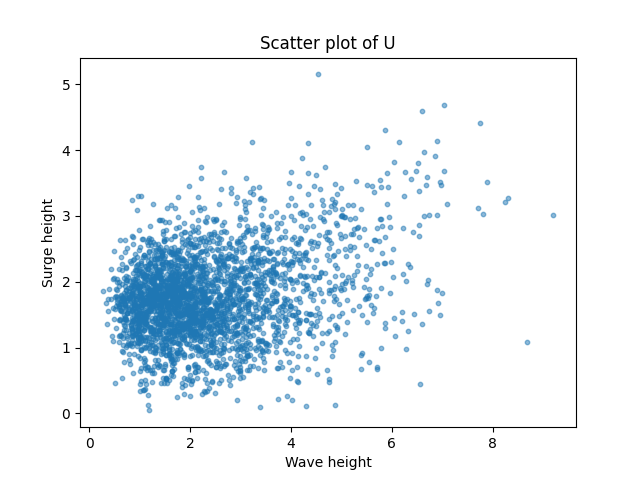
\includegraphics[width=0.5\linewidth]{scatter_plot_U.png}
    \caption{The scatter plot of wavesurge data.}
    \label{fig:scatter_fig}
\end{figure}

We now describe how we calculate test-set estimation in our experiments. By the data generation process, 
\begin{align*}
    \theta^{\text{NETE}} &= \lim_{t\rightarrow\infty}\mathbb{E}[ \frac{W^{\alpha_1}S^{\alpha_2}}{t^{\alpha_1 + \alpha_2}} \mid \|U\| > t] \\
    &= \lim_{t\rightarrow\infty}\mathbb{E}[ \frac{W^{\alpha_1}S^{\alpha_2}}{\|U\|^{\alpha_1 + \alpha_2}} \mid \|U\| > t] \cdot \frac{1}{1 - (\alpha_1 + \alpha_2)\gamma},
\end{align*}
where we use \cref{prop:id} in the second equality. We know the ground-truth $\alpha_1, \alpha_2$ and we can estimate the EVI $\gamma$ using the test set. Suppose the estimated EVI is $\hat{\gamma}$, we set the threshold to $ t_n = 0.25n^{(\hat{\gamma} / (1 + 2 \min \{1, \hat{\gamma} \})} $ and get estimation 

\begin{equation*}
    \hat{\theta}_{\text{test}}^{\text{NETE}} = \mathbb{E}_n[ \frac{W^{\alpha_1}S^{\alpha_2}}{\|U\|^{\alpha_1 + \alpha_2}} \mid \|U\| > t_n] \cdot \frac{1}{1 - (\alpha_1 + \alpha_2)\hat{\gamma}}. 
\end{equation*}
\end{document}
